%%%%%%%%%%%%%%%%%%%%%%%%%%%%%%%%%%%%%%%%%%%%%%%%%%%%%%%%%%%%%%%%%%%%%%%%%%%%%%%%%%%%%
%%%%%%%%%          DOCUMENTO DE UNION DE CAPITULOS                      %%%%%%%%%%%%%
%%%%%%%%%%%%%%%%%%%%%%%%%%%%%%%%%%%%%%%%%%%%%%%%%%%%%%%%%%%%%%%%%%%%%%%%%%%%%%%%%%%%%
%\documentclass[12pt,oneside,a4paper]{book}
\documentclass[twoside,12pt, pdftex]{classes/CUEDthesisPSnPDF}
%{classes/CUEDthesisPSnPDF}

\usepackage{ae}
\usepackage[spanish]{babel}
\selectlanguage{spanish}
\usepackage[OT2,T1]{fontenc}
\usepackage{times}							%%% Uso de letra Time
\usepackage[utf8]{inputenc}				%%% Este paquete permite poner acentos directamente%%% 
\usepackage[pdftex]{graphicx,color}			%%% Inclusion de Figuras 
\usepackage{titlesec}
\usepackage{fancyhdr}
\usepackage{hyperref}
\usepackage{makeidx}
\usepackage{tocbibind} 
\usepackage[intlimits]{amsmath}
\usepackage{cancel}
\usepackage{listings}
\usepackage[usenames,dvipsnames]{color}
\usepackage[final]{stylefiles/mcode}
\usepackage{enumerate}
\usepackage{wasysym}
\usepackage{caption}
\usepackage{graphicx}
\usepackage{subcaption}
\usepackage{booktabs}
\usepackage{glossaries}
\usepackage[gen]{eurosym}
%Macros:

%%%%%%%%%%%%%%% Formato de capítulos %%%%%%%%%%%%%%%%%%%%%
\newcommand{\sublinea}{\titlerule[.3mm] \vspace{.5mm} \titlerule[.75mm]}%
\titleformat{\chapter}[display] %%% definicion a cambiar % 
{\bfseries \sffamily \huge}%%% tipo de letra y tamao     % 
{\filleft                                                % 
 \LARGE \chaptertitlename\ %%% tamao Large               % 
 \Huge \thechapter}%%% n en Large                        % 
{3mm}%%% espacio entre etiqueta y cuerpo                 %
{\filleft}                                               %
[\vspace{0.5mm} \sublinea]                               % 
%%%%%%%%%%%%%%%%%%%%%%%%%%%%%%%%%%%%%%%%%%%%%%%%%%%%%%%%%%

%%%%%%%%%%%%%%% configuracin de pgina %%%%%%%%%%%%%%%%%%
\addtolength{\hoffset}{-5pt}                             %  
\addtolength{\voffset}{-25pt}                            %  
\addtolength{\textwidth}{50pt}                           %
\addtolength{\headheight}{12pt}                          % 
\addtolength{\textheight}{75pt}                          %  
%%%%%%%%%%%%%%%%%%%%%%%%%%%%%%%%%%%%%%%%%%%%%%%%%%%%%%%%%%

%%%%%%%%%%%%%%%%%%%%%%%%%%%%%%%%%%%%%%%%%%%%%%%%%%%%%%%%%%
%%%%%%%%%%%%%%%%% DEFINICIN DE MACROS %%%%%%%%%%%%%%%%%%%%
%%% MACRO FIGURA 										 %
%%%%%%%%%%%%%%%%%%%%%%%%%%%%%%%%%%%%%%%%%%%%%%%%%%%%%%%%%%
% Comando:                                               %
% \figura{nombre-fichero}{argumentos}{titulo}{etiqueta}  %
% argumnetos: width=Xcm,height=Ycm,angle=z               %  
%%%%%%%%%%%%%%%%%%%%%%%%%%%%%%%%%%%%%%%%%%%%%%%%%%%%%%%%%%
\newcommand{\figura}[4]{                                 %
   \begin{figure}[htbp]                                   %
   	\centering                                           %
	\includegraphics[#2]{#1}                             %
	\caption{\footnotesize#3}                            %
	\label{#4}                                           %
\end{figure}                                             %  
             }                                           %

%%%%%%%%%%%%%%%%%%%%%%%%%%%%%%%%%%%%%%%%%%%%%%%%%%%%%%%%%%

\newcommand{\figu}[4]{                                 %
   \begin{figure}[!hp]                                   %
	\centering                                           %
	\includegraphics[#2]{#1}                             %
	\caption{\footnotesize#3}                            %
	\label{#4}                                           %
\end{figure}                                             %  
             }                                           %
%%%%%%%%%%%%%%%%%%%%%%%%%%%%%%%%%%%%%%%%%%%%%%%%%%%%%%%%%%%
%%%%%%%%%%%%%%%%%%%%%%%%%%%%%%%%%%%%%%%%%%%%%%%%%%%%%%%%%%
% MACRO GRAD (Para colocar el simbolo ° ) % 
%%%%%%%%%%%%%%%%%%%%%%%%%%%%%%%%%%%%%%%%%%%%%%%%%%%%%%%%%%

\newcommand{\grad}{\hspace{-2mm}$\phantom{a}^{\circ}$\hspace{1mm}}

%%%%%%%%%%%%%%%%%%%%%%%%%%%%%%%%%%%%%%%%%%%%%%%%%%%%%%%%%%
% MACRO SUMARIO(SOLO PARA SER USADO DENTRO DE CAPITULOS) % 
%%%%%%%%%%%%%%%%%%%%%%%%%%%%%%%%%%%%%%%%%%%%%%%%%%%%%%%%%%
% Comando:                                               %
% \sumario{nombre de referencia de la seccin}            %
% ********** PARA SECCIONES ***************************  %     
%%%%%%%%%%%%%%%%%%%%%%%%%%%%%%%%%%%%%%%%%%%%%%%%%%%%%%%%%%
\newcommand{\sumario}[1]{                                %
\newline                                                 %
\vspace*{2pt}                                            %
\textsc{\ref{#1} $\circ$ \nameref{#1}}                   %
                          }                              %
%%%%%%%%%%%%%%%%%%%%%%%%%%%%%%%%%%%%%%%%%%%%%%%%%%%%%%%%%%
%%%%%%%%%%%%%%%%%%%%%%%%%%%%%%%%%%%%%%%%%%%%%%%%%%%%%%%%%%
% Comando:                                               %
% \subsumario{nombre de referencia de la subseccin}      %
% ********* PARA SUB-SECCIONES ************************* %
%%%%%%%%%%%%%%%%%%%%%%%%%%%%%%%%%%%%%%%%%%%%%%%%%%%%%%%%%%
\newcommand{\subsumario}[1]{                             %
\newline                                                 %
\vspace*{1pt}                                            %
\hspace*{1cm} {\small - \nameref{#1}}                    %
                          }                              %
%%%%%%%%%%%%%%%%%%%%%%%%%%%%%%%%%%%%%%%%%%%%%%%%%%%%%%%%%%
%%%%%%%%%%%%%%%%%%%%%%%%%%%%%%%%%%%%%%%%%%%%%%%%%%%%%%%%%%
% Comando:                                               %
% \subsumario{nombre de referencia de la subseccin}      %
% ********* PARA SUB-SUB-SECCIONES ********************* %
%%%%%%%%%%%%%%%%%%%%%%%%%%%%%%%%%%%%%%%%%%%%%%%%%%%%%%%%%%
\newcommand{\subsubsumario}[1]{                          %
\newline                                                 %
\vspace*{1pt}                                            %
\hspace*{2cm} {\small   \nameref{#1}}                    %
                          }                              %
%%%%%%%%%%%%%%%%%%%%%%%%%%%%%%%%%%%%%%%%%%%%%%%%%%%%%%%%%%
%%%%%%%%%%%%%%%%%%%%%%%%%%%%%%%%%%%%%%%%%%%%%%%%%%%%%%%%%%
% MACRO ECUACIN                                          % 
%%%%%%%%%%%%%%%%%%%%%%%%%%%%%%%%%%%%%%%%%%%%%%%%%%%%%%%%%%
% Comando:                                               %
% \ecu{etiqueta}{contenido}                              %
%%%%%%%%%%%%%%%%%%%%%%%%%%%%%%%%%%%%%%%%%%%%%%%%%%%%%%%%%%
\newcommand{\ecu}[2]{                                    %
  \begin{equation}                                       %
    #2                                      			 %
    \label{#1}                                           %
  \end{equation}           }                             %
%%%%%%%%%%%%%%%%%%%%%%%%%%%%%%%%%%%%%%%%%%%%%%%%%%%%%%%%%%
%%%%%%%%%%%%%%%%%%%%%%%%%%%%%%%%%%%%%%%%%%%%%%%%%%%%%%%%%%
% Referencia de Figura                                   % 
%%%%%%%%%%%%%%%%%%%%%%%%%%%%%%%%%%%%%%%%%%%%%%%%%%%%%%%%%%
% Comando:                                               %
% \reffig{nombre figura}                                 %
%%%%%%%%%%%%%%%%%%%%%%%%%%%%%%%%%%%%%%%%%%%%%%%%%%%%%%%%%%
\newcommand{\reffig}[1]{                                 %
  \textit{Figura \ref{fig:#1}}                           %
                        }                                %
%%%%%%%%%%%%%%%%%%%%%%%%%%%%%%%%%%%%%%%%%%%%%%%%%%%%%%%%%%
%%%%%%%%%%%%%%%%%%%%%%%%%%%%%%%%%%%%%%%%%%%%%%%%%%%%%%%%%%
% Referencia de anexo                                    % 
%%%%%%%%%%%%%%%%%%%%%%%%%%%%%%%%%%%%%%%%%%%%%%%%%%%%%%%%%%
% Comando:                                               %
% \refanex{nombre anexo}                                %
%%%%%%%%%%%%%%%%%%%%%%%%%%%%%%%%%%%%%%%%%%%%%%%%%%%%%%%%%%
\newcommand{\refanex}[1]{                                %
  \textit{Anexo \ref{#1}}			  			     %
}														 %
%%%%%%%%%%%%%%%%%%%%%%%%%%%%%%%%%%%%%%%%%%%%%%%%%%%%%%%%%%
%%%%%%%%%%%%%%%%%%%%%%%%%%%%%%%%%%%%%%%%%%%%%%%%%%%%%%%%%%
% Referencia de Seccion                                  % 
%%%%%%%%%%%%%%%%%%%%%%%%%%%%%%%%%%%%%%%%%%%%%%%%%%%%%%%%%%
% Comando:                                               %
% \refsec{nombre seccion}                                %
%%%%%%%%%%%%%%%%%%%%%%%%%%%%%%%%%%%%%%%%%%%%%%%%%%%%%%%%%%
\newcommand{\refsec}[1]{                                 %
  \textit{Secci\'on \ref{sec:#1}}						 %
}														 %
%%%%%%%%%%%%%%%%%%%%%%%%%%%%%%%%%%%%%%%%%%%%%%%%%%%%%%%%%%
%%%%%%%%%%%%%%%%%%%%%%%%%%%%%%%%%%%%%%%%%%%%%%%%%%%%%%%%%%
% Referencia de subseccion                               % 
%%%%%%%%%%%%%%%%%%%%%%%%%%%%%%%%%%%%%%%%%%%%%%%%%%%%%%%%%%
% Comando:                                               %
% \refsubsec{nombre subseccion}                          %
%%%%%%%%%%%%%%%%%%%%%%%%%%%%%%%%%%%%%%%%%%%%%%%%%%%%%%%%%%
\newcommand{\refsubsec}[1]{                              %
  \textit{Secci\'on \ref{subsec:#1}}                     %
                        }                                %
%%%%%%%%%%%%%%%%%%%%%%%%%%%%%%%%%%%%%%%%%%%%%%%%%%%%%%%%%%
% Referencia de Capitulo                                 % 
%%%%%%%%%%%%%%%%%%%%%%%%%%%%%%%%%%%%%%%%%%%%%%%%%%%%%%%%%%
% Comando:                                               %
% \refcap{nombre seccion}                                %
%%%%%%%%%%%%%%%%%%%%%%%%%%%%%%%%%%%%%%%%%%%%%%%%%%%%%%%%%%
\newcommand{\refcap}[1]{                                 %
  \textit{Cap\'itulo \ref{#1}}							 %
}														 %
%%%%%%%%%%%%%%%%%%%%%%%%%%%%%%%%%%%%%%%%%%%%%%%%%%%%%%%%%%
% Referencia de Ecuacin                                  % 
%%%%%%%%%%%%%%%%%%%%%%%%%%%%%%%%%%%%%%%%%%%%%%%%%%%%%%%%%%
% Comando:                                               %
% \refecu{nombre ecuaci\'on}                             %
%%%%%%%%%%%%%%%%%%%%%%%%%%%%%%%%%%%%%%%%%%%%%%%%%%%%%%%%%%
\newcommand{\refecu}[1]{                                 %
  \textit{Ec\hspace{1mm}\ref{#1}}                        %
                        }                                %
%%%%%%%%%%%%%%%%%%%%%%%%%%%%%%%%%%%%%%%%%%%%%%%%%%%%%%%%%%
%%%%%%%%%%%%%%%%%%%%%%%%%%%%%%%%%%%%%%%%%%%%%%%%%%%%%%%%%%
% Salto de renglon                                       % 
%%%%%%%%%%%%%%%%%%%%%%%%%%%%%%%%%%%%%%%%%%%%%%%%%%%%%%%%%%
% Comando:                                               %
% \salto                                                 %
%%%%%%%%%%%%%%%%%%%%%%%%%%%%%%%%%%%%%%%%%%%%%%%%%%%%%%%%%%
\newcommand{\salto}{                                     % 
\vspace*{11pt}      }                                    %
%%%%%%%%%%%%%%%%%%%%%%%%%%%%%%%%%%%%%%%%%%%%%%%%%%%%%%%%%%

%%%%%%%%%%%%%%%%%%%%%%%%%%%%%%%%%%%%%%%%%%%%%%%%%%%%%%%%%%
\newcommand{\referencia}[1]{                                  %
  \textit{[\cite{#1}]}                           %
                        }      							 %
%%%%%%%%%%%%%%%%%%%%%%%%%%%%%%%%%%%%%%%%%%%%%%%%%%%%%%%%%%

%%%%%%%%%%%%%%%%%%%%%%%%%%%%%%%%%%%%%%%%%%%%%%%%%%%%%%%%%%
% Unidades: Nanosegundos, micro metros, nanómetros, etc.
%
\newcommand{\ns} {\textrm{ns}}
\newcommand{\nanom} {\textrm{nm}}
\newcommand{\microm} {$\mu\textrm{m}$ }
\newcommand{\mmcuadrado} {$\textrm{mm}^2$}
%
%%%%%%%%%%%%%%%%%%%%%%%%%%%%%%%%%%%%%%%%%%%%%%%%%%%%%%%%%%

% Formato de las letras más cómodos.
\newcommand{\negrita}[1]{\textbf{#1}}
\newcommand{\cursi}[1]{\emph{#1}}
\newcommand{\layout}{\emph{layout }}
\newcommand{\netlist}{\emph{netlist }}

% Includes a MATLAB script.
% The first parameter is the label, which also is the name of the script
%   without the .m.
% The second parameter is the optional caption.
\newcommand{\matlabscript}[2]
  {\begin{itemize}\item[]\lstinputlisting[caption=#2,label=#1]{#1.m}\end{itemize}}

\newcommand{\ns} {\textrm{ns}}
\newcommand{\nanom} {\textrm{nm}}
%\newcommand{\microm} {$\mu\textrm{m}$}
\loadglsentries{defns}


%\usepackage{cite}
\ifpdf
    \pdfinfo { /Title  (Diseño de un Sumador Rápido en tecnología CMOS submicrónica utilizando Herramientas de Software Libre)
               /Creator (TeX)
               /Producer (pdfTeX)
               /Author (Leandro Marsó)
               /CreationDate (D:20130606000000)  %format D:YYYYMMDDhhmmss
               /ModDate (D:20131014000000)
               /Subject (Diseño de Circuitos Integrados)
               /Keywords (Circuitos Integrados VLSI Sumador Rápido)}
    
\fi

%\makeindex \label{indice}
\hyphenation{ es-cla-re-ci-mien-to ma-te-ria-li-zar-se} 



\begin{document}
\sloppy

\begin{titlepage}
\pagestyle{empty}       

\begin{center}
	\Huge{Universidad Nacional de Córdoba\\}
	\Large {Facultad de Ciencias Exáctas, Físicas y Naturales}\\

\vspace{1cm}

%	
\includegraphics[width=50mm]{tapa/dibujo.pdf}\\

\includegraphics{tapa/escudo2.pdf}


\vspace{1cm}

%	\textbf{\Large{Marxismo y Feminismo}}\\%[2ex]
%	\large{ ``Textos seleccionados'' }\\

	\Huge \textbf{\\[2ex]Proyecto Integrador}
	\Large \textsl{\\[2ex] '' Diseño de un Sumador Rápido y de Bajo Consumo en tecnología CMOS submicrónica utilizando Herramientas de Software Libre''}

%\begin{flushright}
	\begin{normalsize}
%		\\Compilación de la Cátedra Che Guevara Córdoba 2012}
	\end{normalsize}
	\begin{large}	
		\\ \textbf{Setiembre 2013}
	\end{large}

\end{center}
%\end{flushright}

\vspace{0.5cm}

\begin{center}

%	
\includegraphics[width=50mm]{tapa/escudo2.pdf}
%		\textsl{\\En la Construcción de un Movimiento Político }
%		\\ \uri{http://cordobasemueve.org.ar}


\end{center}

% turn of those nasty overfull and underfull hboxes
\hbadness=10000
\hfuzz=50pt
\end{titlepage}
			%%% INCLUYE DE CARATULA 
\maketitle
%\frontmatter
%% Copyright 2007 by Till Tantau
%
% This file may be distributed and/or modified
%
% 1. under the LaTeX Project Public License and/or
% 2. under the GNU Public License.
%
% See the file doc/licenses/LICENSE for more details.
%%%%%%%%%%%%%%%%%%%%%%%%%%%%%%%%%%%%%%%%%%%%%%%%%%%%%%%%%%
% Unidades: Nanosegundos, micro metros, nan�metros, etc.
%
\newcommand{\ns} {\textrm{ns}}
\newcommand{\nanom} {\textrm{nm}}
\newcommand{\microm} {$\mu\textrm{m}$ }
\newcommand{\micromcuadrado} {$\mu\textrm{m}^2$}
\newcommand{\mmcuadrado} {$\textrm{mm}^2$}

%
%%%%%%%%%%%%%%%%%%%%%%%%%%%%%%%%%%%%%%%%%%%%%%%%%%%%%%%%%%

% Formato de las letras m�s c�modos.
\newcommand{\negrita}[1]{\textbf{#1}}
\newcommand{\cursi}[1]{\emph{#1}}
\newcommand{\layout}{\emph{layout }}
\newcommand{\netlist}{\emph{netlist }}




\documentclass{beamer}

%
% DO NOT USE THIS FILE AS A TEMPLATE FOR YOUR OWN TALKS�!!
%
% Use a file in the directory solutions instead.
% They are much better suited.
%


% Setup appearance:

\usetheme{Darmstadt}
\usefonttheme[onlylarge]{structurebold}
\setbeamerfont*{frametitle}{size=\normalsize,series=\bfseries}
\setbeamertemplate{navigation symbols}{}
\setbeamercovered{transparent}

% Standard packages

\usepackage[spanish]{babel}
\usepackage[latin1]{inputenc}
\usepackage{times}
\usepackage[T1]{fontenc}
\usepackage{booktabs}
\usepackage[gen]{eurosym}
\usepackage{subcaption}
%\usepackage{caption}
\usepackage{wasysym}
\usepackage{listings}
\lstset{%                       % Configuraci�n de par�metros de listing.
  basicstyle=\small\ttfamily,     % C�digos con fuente TrueType.
  breaklines=false,                % Rompe l�neas demasiado largas.
  xrightmargin=1cm,               % Margen derecho.
  %escapeinside=wz,                % Para escapar a LaTeX.
}%

% Setup TikZ

\usepackage{tikz}
\usetikzlibrary{arrows}
\tikzstyle{block}=[draw opacity=0.7,line width=1.4cm]


% Author, Title, etc.

\title[Dise�o de circuitos integrados con Software Libre]
{%
  Dise�o de un Sumador R�pido en tecnolog�a CMOS
  submicr�nica utilizando Herramientas de Software Libre
}

\author[Mars�]
{
  Leandro~Mars�\inst{1} \and
  Pablo~Cayuela~(Director)\inst{2} \and
  Hugo~Carrer~(Codirector)\inst{1} 
}

\institute[UNC and others]
{
  \inst{1}%
  Universidad Nacional de C�rdoba, Argentina
  \and
  \vskip-2mm
  \inst{2}%
  Universidad Tecnol�gica Nacional, FRC, Argentina
  \and
  \vskip-2mm
}

\date[FCEFyN 2006]
{Facultad de Ciencias Ex�ctas, F�sicas y Naturales, 2015}

% Delete this, if you do not want the table of contents to pop up at
% the beginning of each subsection:
\AtBeginSubsection[]
{
    \begin{frame}<beamer>{Temario}
          \tableofcontents[currentsection,currentsubsection]
	    \end{frame}
	  }

% The main document

\begin{document}

\begin{frame}
  \titlepage
\end{frame}

\begin{frame}{Temario}
  \tableofcontents
\end{frame}


\section{Introducci�n}
\subsection{Definiciones generales}
\begin{frame}{�Qu� es un sumador r�pido?}

\end{frame}
%-------------------------------------------------------------
\begin{frame}{�Qu� es un circuito integrado?}
  \begin{figure}
  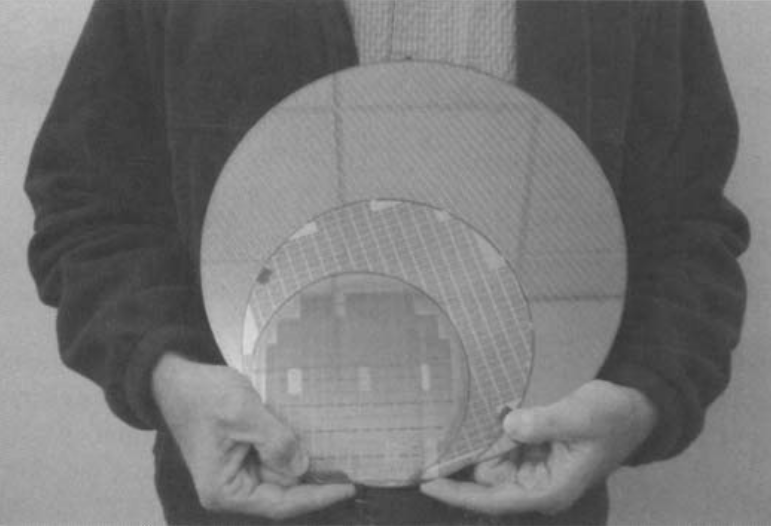
\includegraphics[scale=0.30]{figuras/wafers.png}
  \caption{Obleas de silicio de 150, 200 y 300~mm de d�ametro, de un proceso CMOS.}
  \end{figure}
\end{frame}
%-------------------------------------------------------------
\begin{frame}{�Qu� es un circuito integrado?}
  \begin{figure}
  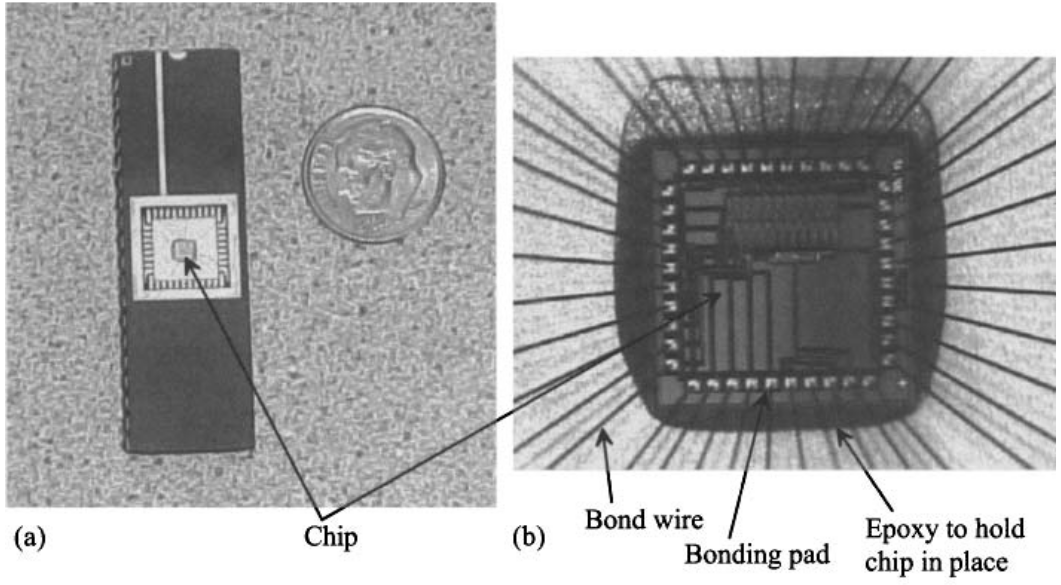
\includegraphics[scale=0.27]{figuras/encapsulado.png}
  \caption{Encapsulado del chip (a) y (b) una vista aumentada.}
  \end{figure}
\end{frame}
%-------------------------------------------------------------
\begin{frame}{�Qu� es un circuito integrado?}
  \begin{figure}
  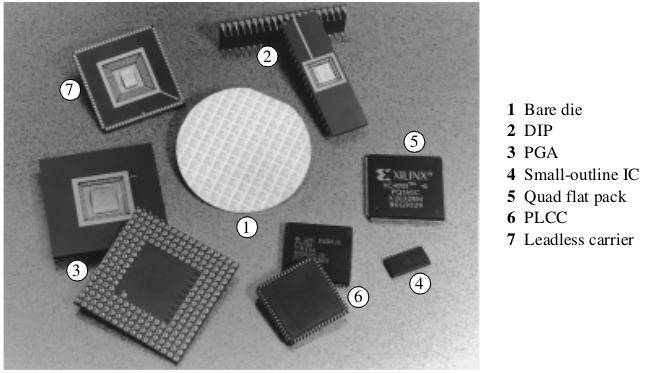
\includegraphics[scale=0.45]{figuras/chips.png}
\caption{Algunos tipos de encapsulados comunes.}
  \end{figure}
\end{frame}
%-------------------------------------------------------------
\begin{frame}{�Qu� es un circuito integrado?}
  \begin{Large}
  \begin{center}
    \textbf{
  �C�mo accedemos a fabricar circuitos integrados?
}
\end{center}
\end{Large}

    \begin{table}[h]
      \centering
      \begin{tabular}{@{}lc@{}}
	\toprule
	\textbf{Fabrica}             & \textbf{Proceso CMOS} \\ \midrule
	TSMC                & 28~nm - 180~nm             \\
	Globalfoundries     & 14~nm - 180~nm             \\
	IBM                 & 32~nm -  250nm            \\
	ON Semi             & 0.35~um - 0.7~um           \\
	Austria Micro Systems & 180~nm - 0.35~um           \\ \bottomrule
      \end{tabular}
      \caption{Procesos disponibles por medio de MOSIS}
      \label{tab:procesosMOSIS}
    \end{table}
\end{frame}
%-------------------------------------------------------------
\begin{frame}{�Qu� es un circuito integrado?}
  \begin{Large}
  \begin{center}
    \textbf{
  �C�mo accedemos a fabricar circuitos integrados?
}
\end{center}
\end{Large}
    \begin{table}[h]
      \centering
      \begin{tabular}{@{}lc@{}}
	\toprule
	\textbf{Fabrica}             & \textbf{Proceso CMOS} \\ \midrule
	STMicroelectronics  & 28~nm - 130~nm             \\
	Austria Micro Systems & 180~nm - 0.35~um           \\ \bottomrule
      \end{tabular}
      \caption{Procesos disponibles por medio de CMP}
      \label{tab:procesosCMP}
    \end{table}

\end{frame}

%-------------------------------------------------------------
\begin{frame}{�Qu� es un circuito integrado?}
  \begin{Large}
  \begin{center}
    \textbf{
  �Cu�nto podemos integrar?
}
\end{center}
\end{Large}

  \begin{columns}[t]
    \column{.43\textwidth}
    \begin{exampleblock}{CMOS 350~nm de AMS}
    \begin{itemize}
      \item 18kGates/mm$^2$
      \item 650~\euro{}/mm$^2$
      \item �rea m�nima 3~mm$^2$
      \item 25 chips
    \end{itemize}
    \end{exampleblock}
    \column{.43\textwidth}
    \begin{exampleblock}{CMOS 180~nm de AMS}
      
    \begin{itemize}
      \item 118~kGates/mm$^2$
      \item 1200~\euro{}/mm$^2$
      \item �rea m�nima 5~mm$^2$
      \item 25 chips
    \end{itemize}
\end{exampleblock}
    \end{columns}
\end{frame}

%-------------------------------------------------------------
\begin{frame}[label=libertades]{�Qu� es el Software Libre?}
\begin{definition}
  �Software libre� es el software que respeta la libertad de los usuarios y la comunidad. A grandes rasgos, significa que los usuarios tienen la libertad de ejecutar, copiar, distribuir, estudiar, modificar y mejorar el software. Es decir, el �software libre� es una cuesti�n de libertad, no de precio.
\end{definition}
\end{frame}
%-------------------------------------------------------------

\begin{frame}{Las cuatro libertades del Software Libre}
Un programa es software libre si los usuarios tienen las cuatro libertades esenciales:
\begin{itemize}
\item<1-> La libertad de ejecutar el programa como se desea, con cualquier prop�sito (libertad 0).
\item<2-> La libertad de estudiar c�mo funciona el programa, y cambiarlo para que haga lo que usted quiera (libertad 1). El \alert{acceso al c�digo fuente} es una condici�n necesaria para ello.
\item<3-> La libertad de redistribuir copias para ayudar a su pr�jimo (libertad 2).
\uncover{\item<4-> La libertad de distribuir copias de sus versiones modificadas a terceros (libertad 3). Esto le permite ofrecer a toda la comunidad la oportunidad de beneficiarse de las modificaciones. El \alert{acceso al c�digo fuente} es una condici�n necesaria para ello.
  }
\end{itemize}
\end{frame}

%-------------------------------------------------------------
%\begin{frame}{Las licencias de uso del software y su importancia}
%  \begin{definition}
%  Algo \alert{alerta} o no.
%
%\end{definition}
%  \hyperlink{libertades<2>}{\beamergotobutton{Cuatro libertades}}
%  \hypertarget{return}{}
%\end{frame}
%-------------------------------------------------------------

\subsection{Planteamiento del problema y motivaci�n}

\begin{frame}{�C�mo dise�ar circuitos integrados con herramientas flexibles y accesibles para todo tipo de uso: acad�mico e industrial?}
  \begin{columns}[t]
    \column{.33\textwidth}
    \begin{exampleblock}{Econ�mico}
      $G\colon$
    \end{exampleblock}
    \column{.33\textwidth}
    \begin{exampleblock}{Acad�mico}
      $G\colon$
    \end{exampleblock}

    \column{.33\textwidth}
    \begin{exampleblock}{Otras razones}
      $G\colon$
    \end{exampleblock}
    \end{columns}

\end{frame}
%-------------------------------------------------------------


%\begin{frame}{What is haplotyping and why is it important?}
%  You hopefully know this after the previous three talks\dots
%\end{frame}
%
%\begin{frame}[t]{General formalization of haplotyping.}
%  \begin{block}{Inputs}
%    \begin{itemize}
%    \item A \alert{genotype matrix} $G$.
%    \item The \alert{rows} of the matrix are \alert{taxa / individuals}.
%    \item The \alert{columns} of the matrix are \alert{SNP sites /
%        characters}. 
%    \end{itemize}
%  \end{block}
%  \begin{block}{Outputs}
%    \begin{itemize}
%    \item A \alert{haplotype matrix} $H$.
%    \item Pairs of rows in $H$ \alert{explain} the rows of $G$.
%    \item The haplotypes in $H$ are \alert{biologically plausible}. 
%    \end{itemize}
%  \end{block}
%\end{frame}
%
%
%\begin{frame}[t]{Our formalization of haplotyping.}
%  \begin{block}{Inputs}
%    \begin{itemize}
%    \item A genotype matrix $G$.
%    \item The rows of the matrix are individuals / taxa.
%    \item The columns of the matrix are SNP sites / characters.
%    \item<alert@1->
%      The problem is directed: one haplotype is known.
%    \item<alert@1->
%      The input is biallelic: there are only two homozygous
%      states (0 and 1) and one heterozygous state (2).
%    \end{itemize}
%  \end{block}
%  \begin{block}{Outputs}
%    \begin{itemize}
%    \item A haplotype matrix $H$.
%    \item Pairs of rows in $H$ explain the rows of $G$.
%    \item<alert@1> The haplotypes in $H$ form a perfect phylogeny.
%    \end{itemize}
%  \end{block}
%\end{frame}
%
%
%\begin{frame}{We can do perfect phylogeny haplotyping efficiently, but
%    \dots}
%  \begin{enumerate}
%  \item \alert{Data may be missing.}
%    \begin{itemize}
%    \item This makes the problem NP-complete \dots
%    \item \dots even for very restricted cases.
%    \end{itemize}
%    \textcolor{green!50!black}{Solutions:}
%    \begin{itemize}
%    \item Additional assumption like the rich data hypothesis. 
%    \end{itemize}
%  \item \alert{No perfect phylogeny is possible.}
%    \begin{itemize}
%    \item This can be caused by chromosomal crossing-over effects.
%    \item This can be caused by incorrect data.
%    \item This can be caused by multiple mutations at the same sites.
%    \end{itemize}
%    \textcolor{green!50!black}{Solutions:}
%    \begin{itemize}
%    \item Look for phylogenetic networks.
%    \item Correct data.
%    \item<alert@1->
%       Find blocks where a perfect phylogeny is possible.
%    \end{itemize}
%  \end{enumerate}
%\end{frame}
%
%
%
%\begin{frame}{How blocks help in perfect phylogeny haplotyping.}
%  \begin{enumerate}
%  \item Partition the site set into overlapping contiguous blocks.
%  \item Compute a perfect phylogeny for each block and combine them.
%  \item Use dynamic programming for finding the partition.
%  \end{enumerate}
%
%  \begin{tikzpicture}
%    \useasboundingbox (0,-1) rectangle (10,2);
%    
%    \draw[line width=2mm,dash pattern=on 1mm off 1mm]
%      (0,1) -- (9.99,1) node[midway,above] {Genotype matrix}
%      (0,0.6666) -- (9.99,0.6666)
%      (0,0.3333) -- (9.99,0.3333)
%      (0,0) -- (9.99,0) node[midway,below] {\only<1>{no perfect phylogeny}};
%
%    \begin{scope}[xshift=-.5mm]
%      \only<2->
%      {
%        \draw[red,block]            (0,.5)   -- (3,.5)
%          node[midway,below] {perfect phylogeny};
%      }
%        
%      \only<3->
%      {
%        \draw[green!50!black,block] (2.5,.5)   -- (7,.5)
%          node[pos=0.6,below] {perfect phylogeny};
%      }
%
%      \only<4->
%      {
%        \draw[blue,block]           (6.5,.5) -- (10,.5)
%          node[pos=0.6,below] {perfect phylogeny};
%      }
%    \end{scope}
%  \end{tikzpicture}
%\end{frame}
%
%\begin{frame}{Objective of the integrated approach.}
%  \begin{enumerate}
%  \item Partition the site set into \alert{noncontiguous} blocks. 
%  \item Compute a perfect phylogeny for each block and combine them. 
%  \item<alert@1-> Compute partition while computing perfect
%    phylogenies. 
%  \end{enumerate}
%
%  \begin{tikzpicture}
%    \useasboundingbox (0,-1) rectangle (10,2);
%
%    \draw[line width=2mm,dash pattern=on 1mm off 1mm]
%      (0,1) -- (9.99,1) node[midway,above] {Genotype matrix}
%      (0,0.6666) -- (9.99,0.6666)
%      (0,0.3333) -- (9.99,0.3333)
%      (0,0) -- (9.99,0) node[midway,below] {\only<1>{no perfect phylogeny}};
%
%    \only<2->
%    {
%      \begin{scope}[xshift=-0.5mm]
%        \draw[red,block] (0,.5)   -- (3,.5) 
%          node[midway,below] {perfect phylogeny}
%                         (8,.5) -- (9,.5);
%
%        \draw[green!50!black,block]
%          (3,.5)   -- (6,.5)
%            node[pos=0.6,below] {perfect phylogeny}
%          (6.4,.5)   -- (8,.5)
%          (9,.5) -- (10,.5);
%
%        \draw[blue,block] (6,.5) -- (6.4,.5)
%          node[midway,below=5mm] {perfect phylogeny};
%      \end{scope}
%    }
%  \end{tikzpicture}
%\end{frame}
%
%
%\begin{frame}{The formal computational problem.}
%
%  We are interested in the computational complexity of \\
%  \alert{the function \alert{$\chi_{\operatorname{PP}}$}}:
%  \begin{itemize}
%  \item It gets genotype matrices as input.
%  \item It maps them to a number $k$.
%  \item This number is minimal such that the sites can be
%    covered by $k$ sets, each admitting a perfect phylogeny.
%    \\
%    (We call this a \alert{pp-partition}.)
%  \end{itemize}
%\end{frame}
%
%
%
%\begin{frame}{Finding pp-partitions of haplotype matrices.}
%  We start with a special case:
%  \begin{itemize}
%  \item The inputs $M$ are \alert{already haplotype matrices}.
%  \item The inputs $M$ \alert{do not allow a perfect phylogeny}.
%  \item What is $\chi_{\operatorname{PP}}(M)$?
%  \end{itemize}
%  \begin{example}
%    \begin{columns}
%      \column{.3\textwidth}
%      $M\colon$
%      \footnotesize
%      \begin{tabular}{cccc}
%        0 & 0 & 0 & 1 \\
%        0 & 1 & 0 & 0 \\
%        1 & 0 & 0 & 0 \\
%        0 & 1 & 0 & 0 \\
%        1 & 0 & 0 & 0 \\
%        0 & 1 & 0 & 1 \\
%        1 & 1 & 0 & 0 \\
%        0 & 0 & 1 & 0 \\
%        1 & 0 & 1 & 0
%      \end{tabular}%
%      \only<2>
%      {%
%        \begin{tikzpicture}
%          \useasboundingbox (2.9,0);
%
%          \draw [red, opacity=0.7,line width=1cm] (1.7 ,1.9) -- (1.7 ,-1.7);
%          \draw [blue,opacity=0.7,line width=5mm] (0.85,1.9) -- (0.85,-1.7)
%                                                  (2.55,1.9) -- (2.55,-1.7);
%        \end{tikzpicture}
%      }
%      \column{.6\textwidth}
%      \begin{overprint}
%        \onslide<1>
%        No perfect phylogeny is possible.
%        
%        \onslide<2>
%        \textcolor{blue!70!bg}{Perfect phylogeny}
%        
%        \textcolor{red!70!bg}{Perfect phylogeny}
%        
%        $\chi_{\operatorname{PP}}(M) = 2$.
%        
%      \end{overprint}
%    \end{columns}
%  \end{example}
%\end{frame}
%
%\begin{frame}{Bad news about pp-partitions of haplotype matrices.}
%  \begin{theorem}
%    Finding \alert{optimal pp-partition of haplotype matrices}\\
%    is equivalent to finding \alert{optimal graph colorings}.
%  \end{theorem}
%
%  \begin{proof}[Proof sketch for first direction]
%    \begin{enumerate}
%    \item Let $G$ be a graph.
%    \item Build a matrix with a column for each vertex of $G$.
%    \item For each edge of $G$ add four rows inducing\\the
%      submatrix $\left(
%        \begin{smallmatrix}
%          0 & 0 \\
%          0 & 1 \\
%          1 & 0 \\
%          1 & 1
%        \end{smallmatrix}\right)$.
%    \item The submatrix enforces that the columns lie in different
%      perfect phylogenies. \qedhere  
%    \end{enumerate}
%  \end{proof}
%\end{frame}
%
%\begin{frame}{Implications for pp-partitions of haplotype matrices.}
%  \begin{corollary}
%    If $\chi_{\operatorname{PP}}(M) = 2$ for a haplotype matrix $M$,
%    we can find an optimal pp-partition in polynomial time. 
%  \end{corollary}
%
%  \begin{corollary}
%    Computing $\chi_{\operatorname{PP}}$ for haplotype matrices is
%    \begin{itemize}
%    \item $\operatorname{NP}$-hard,
%    \item not fixed-parameter tractable, unless
%      $\operatorname{P}=\operatorname{NP}$, 
%    \item very hard to approximate.
%    \end{itemize}
%  \end{corollary}
%\end{frame}
%
%\subsection{Distintas arquitecturas de sumadores}
%
%
%%\subsection{Hardness of PP-Partitioning of Genotype Matrices}
%
%
%\begin{frame}{Finding pp-partitions of genotype matrices.}
%  Now comes the general case:
%  \begin{itemize}
%  \item The inputs $M$ are \alert{genotype matrices}.
%  \item The inputs $M$ \alert{do not allow a perfect phylogeny}.
%  \item What is $\chi_{\operatorname{PP}}(M)$?
%  \end{itemize}
%  \begin{example}
%    \begin{columns}
%      \column{.3\textwidth}
%      $M\colon$
%      \footnotesize
%      \begin{tabular}{cccc}
%        2 & 2 & 2 & 2 \\
%        1 & 0 & 0 & 0 \\
%        0 & 0 & 0 & 1 \\
%        0 & 0 & 1 & 0 \\
%        0 & 2 & 2 & 0 \\
%        1 & 1 & 0 & 0 
%      \end{tabular}%
%      \only<2>
%      {%
%        \begin{tikzpicture}
%          \useasboundingbox (2.9,0);
%          
%          \draw [red, opacity=0.7,line width=1cm] (1.7 ,1.3) -- (1.7 ,-1.1);
%          \draw [blue,opacity=0.7,line width=5mm] (0.85,1.3) -- (0.85,-1.1)
%                                                  (2.55,1.3) -- (2.55,-1.1);
%        \end{tikzpicture}
%      }
%      \column{.6\textwidth}
%      \begin{overprint}
%        \onslide<1>
%        No perfect phylogeny is possible.
%        
%        \onslide<2>
%        \textcolor{blue!70!bg}{Perfect phylogeny}
%        
%        \textcolor{red!70!bg}{Perfect phylogeny}
%        
%        $\chi_{\operatorname{PP}}(M) = 2$.
%        
%      \end{overprint}
%    \end{columns}
%  \end{example}
%\end{frame}
%
%
%\begin{frame}{Bad news about pp-partitions of haplotype matrices.}
%  \begin{theorem}
%    Finding \alert{optimal pp-partition of genotype matrices}
%    is at least as hard as finding \alert{optimal colorings of
%      3-uniform hypergraphs}. 
%  \end{theorem}
%
%  \begin{proof}[Proof sketch]
%    \begin{enumerate}
%    \item Let $G$ be a 3-uniform hypergraph.
%    \item Build a matrix with a column for each vertex of $G$.
%    \item For each hyperedge of $G$ add four rows inducing\\ the submatrix
%      $\left(
%        \begin{smallmatrix}
%          2 & 2 & 2 \\
%          1 & 0 & 0 \\
%          0 & 1 & 0 \\
%          0 & 0 & 1
%        \end{smallmatrix}\right)
%      $.
%    \item The submatrix enforces that the three columns do not all lie
%      in the same perfect phylogeny. \qedhere
%    \end{enumerate}
%  \end{proof}
%\end{frame}
%
%\begin{frame}{Implications for pp-partitions of genotype matrices.}
%  \begin{corollary}
%    Even if we know $\chi_{\operatorname{PP}}(M) = 2$ for a genotype matrix $M$,\\
%    finding a pp-partition of any fixed size is still
%    \begin{itemize}
%    \item $\operatorname{NP}$-hard,
%    \item not fixed-parameter tractable, unless
%      $\operatorname{P}=\operatorname{NP}$, 
%    \item very hard to approximate.
%    \end{itemize}
%  \end{corollary}
%\end{frame}
%

\section{Implementaci�n}

\subsection{Dise�o digital}
\begin{frame}{Dise�o digital}
  Selecci�n de la arquitectura.

\begin{figure}[h]
  \centering
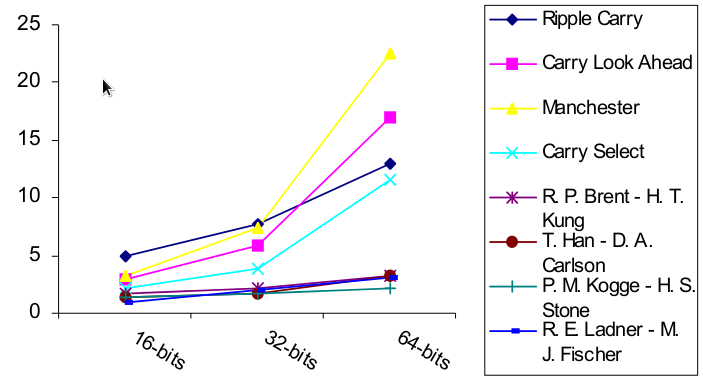
\includegraphics[scale=0.39]{figuras/retardo-bits.png}
  \caption{Retardo respecto al tama�o de los operandos}
  \label{retardo-bits}
\end{figure}


\end{frame}
\begin{frame}{Dise�o digital}
  Selecci�n de la arquitectura.

\begin{figure}[h]
  \centering
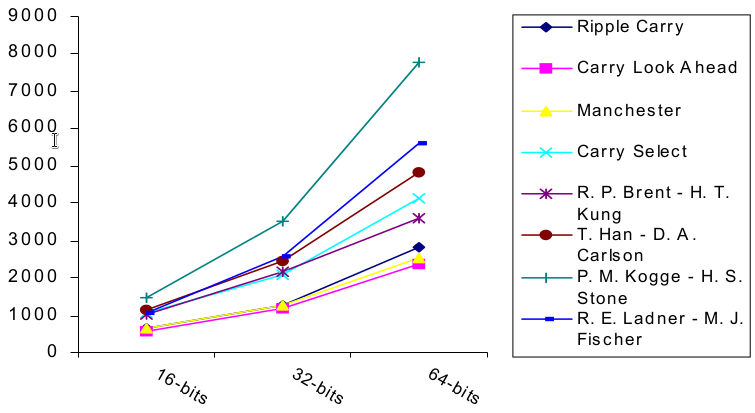
\includegraphics[scale=0.39]{figuras/area-bits.png}
\vspace{-1pt}
  \caption{�rea respecto al tama�o de los operandos}
  \label{area-bits}
\vspace{-15pt}
\end{figure}
\end{frame}

\begin{frame}{}
\begin{table}[h]
\centering
\begin{tabular}{|l|l|l|}
\hline
\multicolumn{1}{|c|}{\textbf{Arquitectura}} & \multicolumn{1}{c|}{\textbf{Retardo M�x.   }} & \multicolumn{1}{c|}{\textbf{�rea}} \\ \hline
Ripple Carry  & \(O(n)\) & \(O(n)\) \\ \hline
Carry Look-Ahead  & \(O(\log_2(n))\) & \(O(n\log_2(n))\) \\ \hline
Ladner-Fisher &\( O(\log_2(n))\) & \(O(n\log_2(n))   \) \\ \hline
Sklansky &\( O(\log_2(n))\) & \(O(n\log_2(n))\) \\ \hline
Kogge-Stone & \( O(\log_2(n))\) & \(O(n\log_2n)\)\\ \hline
%Han-Carlson & \( O(\log_2(n))\) &... \\ \hline % Lo quito ya que no encuentro la funci�n de complejidad de �rea.
Brent-Kung & $O(\log_2(n))$ & \(O(n)\) \\ \hline
\end{tabular}
\caption{Resumen de las funciones de retardo y �rea de algunos sumadores}\label{tabla:sumadores}
\end{table}
\hyperlink{sumadorPP}{\beamergotobutton{Implementaci�n}}
  \hypertarget{return}{}

\end{frame}
%----------------------------------------------------------------------------------
\begin{frame}{Carry Look-ahead}

Ya que una vez que el acarreo en la posici�n \(i\) es conocido, se puede calcular la suma como:
\begin{equation}\label{s_i}
s_i = a_i \oplus b_i\oplus c_i
\end{equation}

El acarreo se \emph{genera} � se \emph{propaga}, seg�n las siguientes ecuaciones:

%\vee es el OR
%\wedge es el AND
%\oplus es el XOR
%$$a_i=\lnot{a_i}\wedge\lnot{b_i}=\lnot{(a_i \vee b_i)}$$
$$g_i=a_ib_i$$
$$p_i=a_i \oplus b_i$$

C�lculo recursivo del acarreo:
\begin{equation}
%c_{i+1}=g_i\vee (c_i \wedge p_i)
c_{i+1}=g_i + c_i p_i
\end{equation}

\end{frame}
%----------------------------------------------------------------------------------
\begin{frame}{Desenrollando la recurrencia del acarreo}
Uno puede desenrollar esta f�rmula recursiva del acarreo hasta lograr una funci�n que dependa directamente de los operandos ($a$ y $b$) y del acarreo de entrada $c_{\text{in}}$:
\scriptsize{
\begin{equation}
\begin{aligned}
c_i &= g_{i-1} + p_{i-1}c_{i-1}\notag\\
&=g_{i-1}+p_{i-1}(g_{i-2}+p_{i-2}c_{i-2})=g_{i-1}+p_{i-1}g_{i-2}+p_{i-1}p_{i-2}c_{i-2}\notag\\
&=g_{i-1} + p_{i-1}g_{i-2}+p_{i-1}p_{i-2}g_{i-3}+p_{i-1}p_{i-2}p_{i-3}c_{i-3}\notag\\
&=g_{i-1} +p_{i-1}g_{i-2}+p_{i-1}p_{i-2}g_{i-3}+p_{i-1}p_{i-2}p_{i-3}g_{i-4}+p_{i-1}p_{i-2}p_{i-3}p_{i-4}c_{i-4}\label{gyp}	
\end{aligned}
\end{equation}
}
\end{frame}

%----------------------------------------------------------------------------------
\begin{frame}
Podemos interpretar estas ecuaciones de la siguiente forma: las cuatro posiciones de bits propagan colectivamente un acarreo $c_\text{in}$ si y solo s� cada una de las posiciones propaga; y el bloque gener	a un acarreo si en la posici�n $i+3$ se genera uno, o se podrouce en la posici�n $i+2$ y es propagado por la posici�n $i+3$, etc.
\end{frame}
%----------------------------------------------------------------------------------
\begin{frame}{Problema de prefijos paralelos}

\begin{equation}
\begin{aligned}
\text{Dado:}\\
 & \text{Entradas:} x_0,x_1,\dotsc,x_{k-1} \\
 & \text{Un operador + asociativo}\\ 
\text{Computar}:&x_0 \nonumber \\
&x_0+x_1 \nonumber \\ 
&x_0+x_1+x_2 \nonumber \\ 
&\vdots \nonumber \\ 
&x_0+x_1+x_2+\dotsb+x_{k-1} \nonumber
\end{aligned}
\end{equation}

\end{frame}


%----------------------------------------------------------------------------------
\begin{frame}{C�mputo del acarreo como un problema de prefijos paralelos}
 
Pensemos la ecuaci�n \ref{gyp} de la siguiente forma, asumiendo que $c_0=c_\text{in}$ viene desde otro bloque:
\begin{equation}
\begin{aligned}
g_{[i,i+3]} &= g_{i+3}+g_{i+2}p_{i+3}+g_{i+1}p_{i+2}p_{i+3}+g_{i}p_{i+1}p_{i+2}p_{i+3}\nonumber\\
p_{[i,i+3]} &= p_{i}p_{i+1}p_{i+2}p_{i+3}\nonumber
\end{aligned}
\end{equation}
\end{frame}
%----------------------------------------------------------------------------------

\begin{frame}{C�mputo del acarreo como un problema de prefijos paralelos}
  \scriptsize{
\begin{equation}\label{eq:ppProblem}
\begin{aligned}
\text{Dados:}\\
 & \text{Entradas:} (g_0,p_0),(g_1,p_1),\dotsc,(g_{k-1},p_{k-1}) \\
 & \text{Un operador} \circ \text{asociativo}\\ 
\text{Computar}:\\
(G_0,P_0) = &(g_{[0,0]},p_{[0,0]})\\
(G_1,P_1) = &(g_{[0,0]},p_{[0,0]})\circ(g_{[0,1]},p_{[0,1]})\\
&\vdots  \\
(G_{k-1},P_{k-1}) = &(g_{[0,0]},p_{[0,0]})\circ(g_{[0,1]},p_{[0,1]})\dotsc \circ(g_{[0,k-2]},p_{[0,k-2]})\circ(g_{[0,k-1]},p_{[0,k-1]}) \nonumber
\end{aligned}
\end{equation}
}
\end{frame}
%-------------------------------------------------------------------------
\begin{frame}{Operador de Brent-Kung}
El operador $\circ$ se define como:
\begin{equation}
(g,p) \circ (\hat{g},\hat{p}) = (g\vee(p\wedge\hat{g}),p\wedge\hat{g})\label{gap}
\end{equation}

\begin{figure}[h!]
  \centering
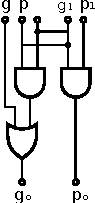
\includegraphics[scale=1.0]{figuras/dotOp_schem.pdf}
%\vspace{-5pt}
  \caption{Operator Punto de Brent-Kung}
  \label{dotOp}
%\vspace{-15pt}
\end{figure}
\end{frame}
%-------------------------------------------------------------------------

\begin{frame}[label=sumadorPP]
\begin{figure}[h]
  \centering
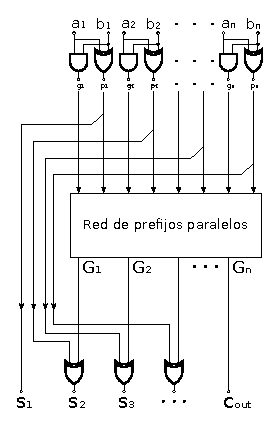
\includegraphics[scale=1.0]{figuras/arquitectura_schem_generico.eps}
  \caption{Sumador de prefijo paralelo}
  \label{fig:ppadder}
\end{figure}

\end{frame}
%----------------------------------------------------------------------------------
\begin{frame}

\begin{figure}[h!]
\vspace{-5pt}
  \centering
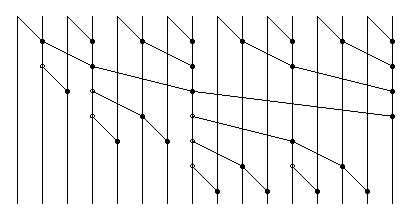
\includegraphics[scale=1.4]{figuras/bKung16.eps}
  \caption{Red de prefijo paralelo para Brent-Kung (ejemplo de 16 bits)}
\label{bKung16}
\vspace{-10pt}
\end{figure}

\end{frame}
%-------------------------------------------------------------------------
\begin{frame}
\begin{figure}[h]
  \centering
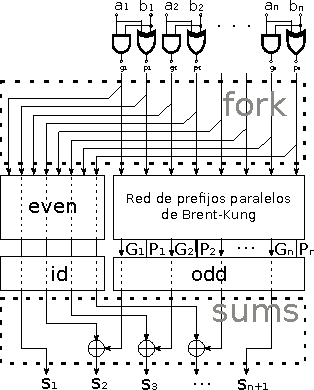
\includegraphics[scale=1.0]{figuras/arquitectura_schem.pdf}
  \caption{Sumador de Brent-Kung}
  \label{fig:bkungadder}
\end{figure}
\end{frame}
%-------------------------------------------------------------------------


\begin{frame}
\begin{figure}[h!]
\vspace{-5pt}
  \centering
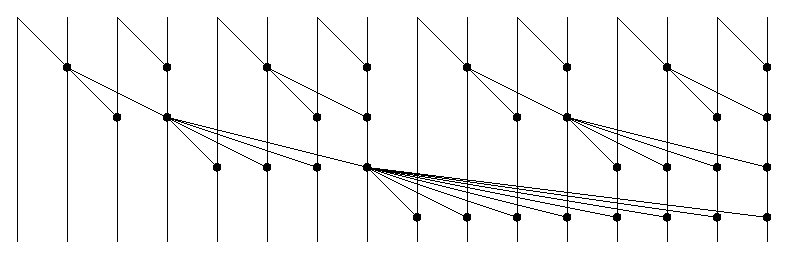
\includegraphics[scale=0.7]{figuras/sklansky16.eps}
  \caption{Red de prefijo paralelo para Sklansky (ejemplo de 16 bits)}
\label{fig:sklansky16}
\vspace{-10pt}
\end{figure}\end{frame}

%-------------------------------------------------------------------------
\begin{frame}{Implementaci�n de los circuitos en lenguaje de descripci�n de hardware}
\end{frame}
%-------------------------------------------------------------------------
\begin{frame}{Nuevos lenguajes de descripci�n de hardware}
 \begin{itemize}
    \item Usar un �nico lenguaje para describir, simular, verificar e implementar el circuito
    \item Los circuitos se describen en Haskell, Scala o Python, el HDL es simplemente un conjunto de m�dulos o librer�as
    \item Generar autom�ticamente una descripci�n en VHDL o Verilog
    \item Describir circuitos que construimos a partir de subcircuitos, adem�s de la posibilidad de reutilizar f�cilmente patrones de conexi�n
 \end{itemize}


\end{frame}
%-------------------------------------------------------------------------

\begin{frame}{�Por qu� Lava?}
  \begin{itemize}
    \item Conocimiento previo del lenguaje
    \item Genera un netlist VHDL (F�cil integraci�n con Electric)
    \item Los circuitos son descriptos como funciones que operan sobre listas, tuplas o sobre circuitos
    \item F�cil integraci�n con un SAT solver para verificaci�n formal
  \end{itemize}

\end{frame}
%-------------------------------------------------------------------------

\begin{frame}[fragile]{Operador de Brent-Kung en Lava}
A partir de la definici�n del operador:
\begin{equation*}
(g,p) \circ (\hat{g},\hat{p}) = (g\vee(p\wedge\hat{g}),p\wedge\hat{g})\label{gap}
\end{equation*}
En Lava la escribimos:

\lstset{language=Haskell}
\begin{lstlisting}
dotOp ((g1, p1) ,(g, p)) = (go, po)
   where
      go = or2 (g, and2 (p, g1))
      po = and2 (p, p1)
\end{lstlisting}
\end{frame}
%-------------------------------------------------------------------------
\begin{frame}[fragile]{Red de prefijo paralelo de Brent-Kung en Lava}
Funciones auxiliares:
  \begin{figure}
    \centering
    
\includegraphics[scale=2.00]{figuras/wrapR.eps}
 \end{figure}
\end{frame}
%-------------------------------------------------------------------------
\begin{frame}[fragile]
  \begin{lstlisting}
comb []     = []
comb [a]    = []
comb (a:as) = dop [a, head as] ++ comb (tail as)
--
posComb (a:as)  = a: (comb (init as))++ [last as]
--
half p = unzipl ->- (id -|- p) ->- zipl
--
wrap p = comb ->- half p ->- posComb 
\end{lstlisting}
\end{frame}
%-------------------------------------------------------------------------
\begin{frame}[fragile]
\noindent Luego finalemente, podemos describir {\verb|ppNet|}:

 \begin{figure}
    \centering
    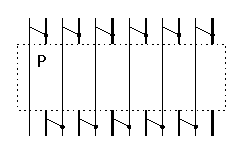
\includegraphics[scale=2.0]{figuras/sheeranrecurrence.eps}
 \end{figure}

\begin{lstlisting}
ppNet [a]    = []
ppNet [a, b] = dop [a, b]
ppNet as     = wrap ppNet as
\end{lstlisting}

\end{frame}
%-------------------------------------------------------------------------






%\begin{frame}{Automatic optimal pp-partitioning is hopeless, but\dots}
%  \begin{itemize}
%  \item The hardness results are \alert{worst-case} results for\\
%    \alert{highly artificial inputs}.
%  \item \alert{Real biological data} might have special properties
%    that make the problem \alert{tractable}.
%  \item One such property is that perfect phylogenies are often
%    perfect \alert{path} phylogenies:
%
%    In HapMap data, in 70\% of the blocks where a perfect phylogeny
%    is possible a perfect path phylogeny is also possible.
%  \end{itemize}  
%\end{frame}
%
%
%\begin{frame}{Example of a perfect path phylogeny.}
%  \begin{columns}[t]
%    \column{.3\textwidth}
%    \begin{exampleblock}{Genotype matrix}
%      $G\colon$
%      \begin{tabular}{ccc}
%        A & B & C \\\hline
%        2 & 2 & 2 \\
%        0 & 2 & 0 \\
%        2 & 0 & 0 \\
%        0 & 2 & 2 
%      \end{tabular}
%    \end{exampleblock}
%
%    \column{.3\textwidth}
%    \begin{exampleblock}{Haplotype matrix}
%      $H\colon$
%      \begin{tabular}{ccc}
%        A & B & C \\\hline
%        1 & 0 & 0 \\
%        0 & 1 & 1 \\
%        0 & 0 & 0 \\
%        0 & 1 & 0 \\
%        0 & 0 & 0 \\
%        1 & 0 & 0 \\
%        0 & 0 & 0 \\
%        0 & 1 & 1 
%      \end{tabular}
%    \end{exampleblock}
%
%    \column{.4\textwidth}
%    \begin{exampleblock}{Perfect path phylogeny}
%      \begin{center}
%        \begin{tikzpicture}[auto,thick]
%          \tikzstyle{node}=%
%          [%
%            minimum size=10pt,%
%            inner sep=0pt,%
%            outer sep=0pt,%
%            ball color=example text.fg,%
%            circle%
%          ]
%        
%          \node [node] {} [->]
%            child {node [node] {} edge from parent node[swap]{A}}
%            child {node [node] {}
%              child {node [node] {} edge from parent node{C}}
%              edge from parent node{B}
%            };
%        \end{tikzpicture}
%      \end{center}
%    \end{exampleblock}
%  \end{columns}
%\end{frame}
%
%
%\begin{frame}{The modified formal computational problem.}
%  We are interested in the computational complexity of \\
%  the function $\chi_{\alert{\operatorname{PPP}}}$:
%  \begin{itemize}
%  \item It gets genotype matrices as input.
%  \item It maps them to a number $k$.
%  \item This number is minimal such that the sites can be
%    covered by $k$ sets, each admitting a perfect \alert{path} phylogeny.
%    \\
%    (We call this a ppp-partition.)
%  \end{itemize}
%\end{frame}
%-------------------------------------------------------------
\subsection{Dise�o f�sico}
\begin{frame}{Flujo de dise�o f�sico}
\begin{figure}[h]
\centering
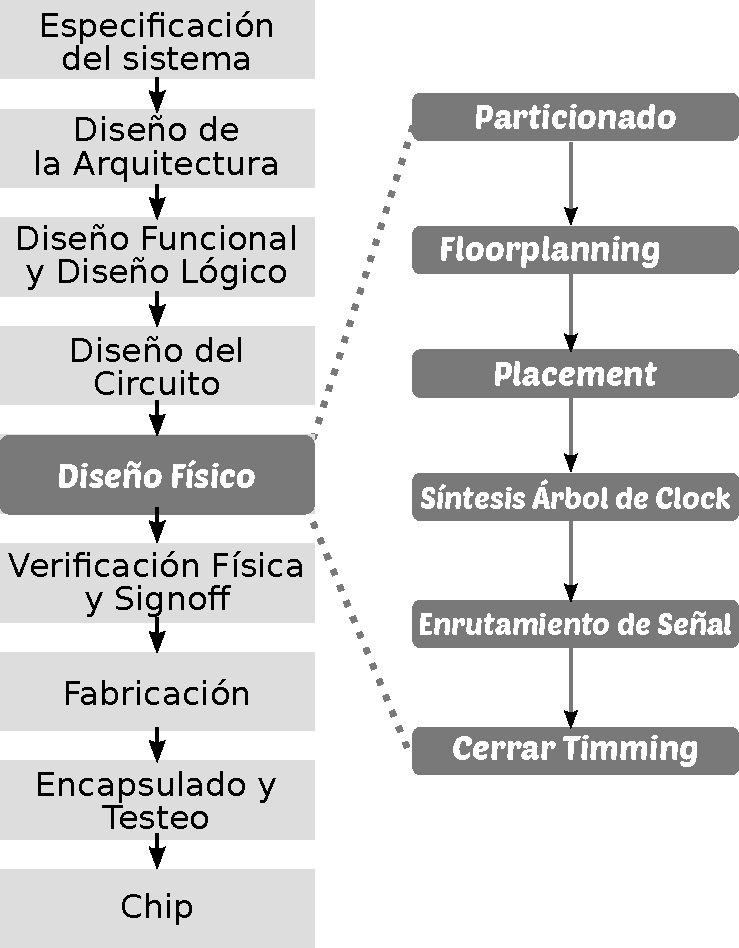
\includegraphics[scale=0.43]{figuras/DisenioFisico.pdf}
  \label{fig:dise�oF�sico}
\end{figure}
\end{frame}
%------------------------------------------------------------
\begin{frame}{Selecci�n del proceso de fabicaci�n}
  Seleccionamos TSMC 180nm por las siguientes razones:
  \begin{itemize}
      \item Existen herramientas de software libre para esta tecnolog�a.
      \item Bajo costo de fabricaci�n 
      \item Posibilidad de integrar sistemas de gran complejidad y alta performance
    \end{itemize}

\end{frame}
%-------------------------------------------------------------
\begin{frame}{Selecci�n del proceso de fabicaci�n}
Ejemplos de microprocesadores que fueron fabricados en esta tecnolog�a:

\begin{table}[h]
\centering
\begin{tabular}{@{}lc@{}}
\toprule
Procesador             & A�o de lanzamiento \\ \midrule
Intel Coppermine E                & 1999             \\
AMD Athlon Thunderbird      & 2000             \\
Intel Celeron (Willamette)               & 2002            \\
Motorola PowerPC 7445 y 7455 (Apollo 6) & 2002           \\ \bottomrule
\end{tabular}
\caption{Procesadores fabricados en CMOS 180nm }
\label{tab:procesadores180nm}
\end{table}
\end{frame}
%-------------------------------------------------------------
\begin{frame}{}
\end{frame}
%-------------------------------------------------------------
\begin{frame}{Reglas de dise�o para TSMC 180nm}
  MOSIS denomina a las reglas de dise�o \textbf{SCN6M\_DEEP}, que significa:
%El proceso nos ofrece 6 capas de metal (aluminio) para la interconexi�n, 1 capa de silicio policristalino (\emph{poly}) para crear la compuerta y tambi�n para la interconexi�n de las mismas (distancias cortas s�lamente, por su mayor resistividad que el cobre), con 2 tipos de �xidos para crear el aislante de las compuertas, los que pueden ser alimentados con tensi�n m�xima de 1,8V, y los que pueden ser alimentados con 3,3V (pensados principalmente como transistores para los circuitos de entrada y salida del chip). MOSIS denomina a las reglas de dise�o que utilizaremos para esta tecnolog�a como SCN6M\_DEEP, que significa:\begin{frame}{180nm TSMC}
  \begin{itemize}
    \item S: Escalable
    \item C: Tecnolog�a de fabricaci�n CMOS
    \item N: Pozo N.
    \item 6M: 6 metales y un conductor policristalino (\emph{poly}) para crear las compuertas.
    \item DEEP: Reglas \emph{deep submicron} (lamda 90nm).
  \end{itemize}
\end{frame}
%-------------------------------------------------------------
\begin{frame}{Mapeo de l�gica a compuertas}
Mapeo de una funci�n l�gica a una celda est�ndar
\begin{figure}[h]
\centering
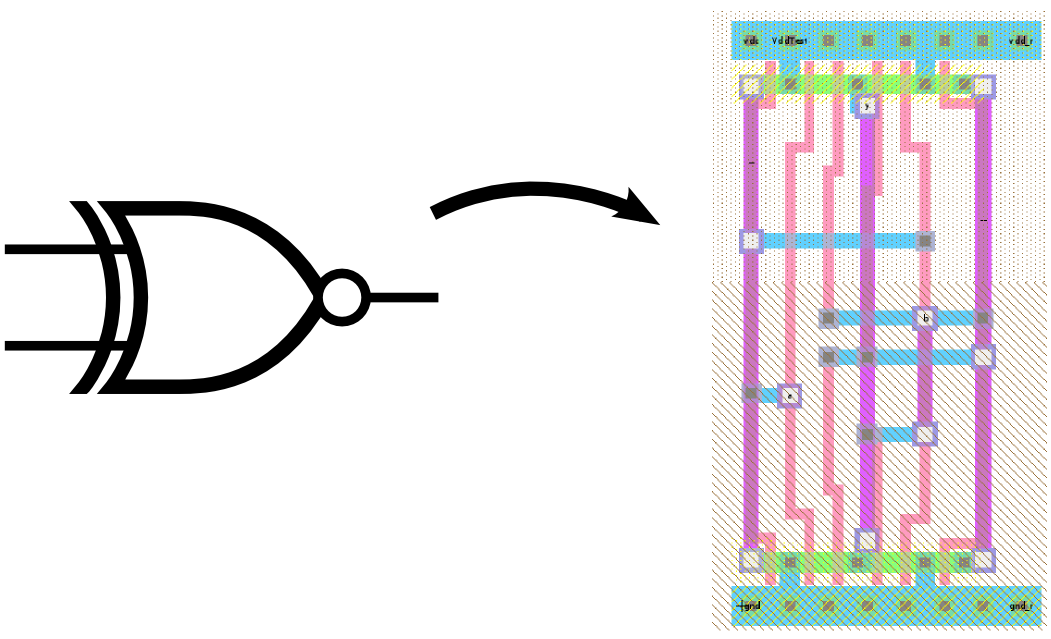
\includegraphics[scale=0.59]{figuras/map-xnor.png}
  \label{fig:map-xnor}
\end{figure}
\end{frame}
%------------------------------------------------------------
\begin{frame}{Librer�a de celdas est�ndar}
\begin{figure}
        \centering
        \begin{subfigure}[b]{0.20\textwidth}
                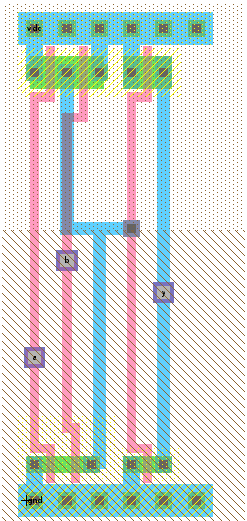
\includegraphics[width=1.075\textwidth]{figuras/and2_1x.png}
                \caption{and2}
                \label{fig:gull}
        \end{subfigure}\quad
        \begin{subfigure}[b]{0.20\textwidth}
                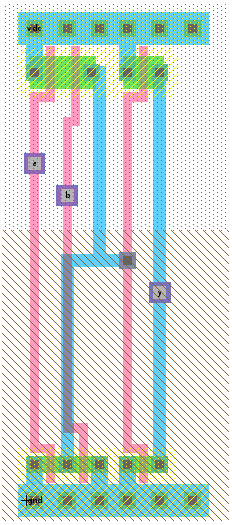
\includegraphics[width=1\textwidth]{figuras/or2_1x.png}
                \caption{or2}
                \label{fig:tiger}
        \end{subfigure} 
        \begin{subfigure}[b]{0.20\textwidth}
                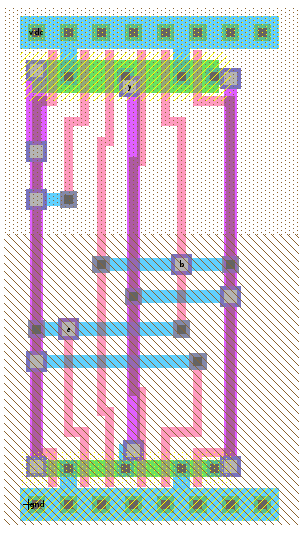
\includegraphics[width=1.31\textwidth]{figuras/xor2_1x.png}
                \caption{xor}
                \label{fig:mouse}
        \end{subfigure}\qquad
        \begin{subfigure}[b]{0.20\textwidth}
                \includegraphics[width=0.845\textwidth]{figuras/id_1x_.png}
                \caption{buffer}
                \label{fig:mouse}
        \end{subfigure}
        \caption{Conjunto de celdas est�ndar}\label{fig:animals}
\end{figure}
\end{frame}

%------------------------------------------------------------

\begin{frame}{Celdas est�ndar}
Grilla de interconexionado y riel de alimentaci�n de las celdas est�ndar de $128 \lambda$
 \begin{figure}[h]
\centering
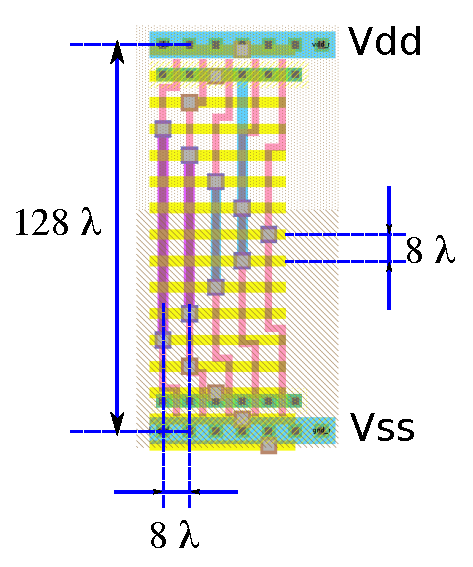
\includegraphics[scale=.7]{figuras/CeldEstandarAlto.eps}
  \label{fig:pitchCeldaEstandar}
\end{figure}
\end{frame}
%------------------------------------------------------------



\begin{frame}{Ubicaci�n y conexionado del \textit{ripple carry adder}}
\begin{table}[h]
\centering
\resizebox{\textwidth}{!}{%
\begin{tabular}{@{}cccc|ccc|ccc@{}}
\toprule
\multicolumn{1}{l}{\textbf{Ripple Carry}} & \multicolumn{3}{c}{8 bits}    & \multicolumn{3}{c}{16 bits}      & \multicolumn{3}{c}{32 bits}      \\ \midrule
filas                                     & 3      & \alert{4}      & 5      & 5       & \alert{6}       & 7       & \alert{8}       & 7       & 6       \\
ancho                                     & 1297   & 966    & 843    & 1562    & 1350    & 1142    & 1881    & 2169    & 2581    \\
alto                                      & 665    & 839    & 958    & 1227    & 1196    & 1600    & 2000    & 1850    & 1360    \\
�rea                                      & 862505 & 810474 & 807594 & 1916574 & 1614600 & 1827200 & 3762000 & 4012650 & 3510160 \\
ancho/alto                                & 0,51   & 0,87   & 1,14   & 0,79    & 0,89    & 1,40    & 1,06    & 0,85    & 0,53    \\ \bottomrule
\end{tabular}
}
\caption{Las dimensiones de los lados y el �rea est�n en $\lambda$ y $\lambda^2$ respectivamente.}
\label{tab:rippleCarry}
\end{table}

\end{frame}
%------------------------------------------------------------
\begin{frame}{Ubicaci�n y conexionado del sumador de \textit{Brent-Kung}}
\begin{table}[h]
\centering
\resizebox{\textwidth}{!}{%
\begin{tabular}{@{}cccc|cccc|cccc@{}}
\toprule
\textbf{Brent-Kung} & \multicolumn{3}{c}{8 bits}      & \multicolumn{4}{c}{16 bits}                & \multicolumn{4}{c}{32 bits}                \\ \midrule
filas               & 3       & \alert{4}     & 5       & 4       & 5       & \alert{6}       & 7       & 6       & \alert{7}       & 8       & 9       \\
ancho               & 1386    & 1090   & 945     & 2268    & 1757    & 1545    & 1429    & 3196    & 1983    & 2569    & 2424    \\
alto                & 746     & 910    & 1199    & 1255    & 1436    & 1540    & 1959    & 2024    & 2871    & 2927    & 2882    \\
�rea                & 1033956 & 991900 & 1133055 & 2846340 & 2523052 & 2379300 & 2799411 & 6468704 & 5693193 & 7519463 & 6985968 \\
ancho/alto          & 0,54    & 0,83   & 1,27    & 0,55    & 0,82    & 1,00    & 1,37    & 0,63    & 1,45    & 1,14    & 1,19    \\ \bottomrule
\end{tabular}
}
\caption{Las dimensiones de los lados y el �rea est�n en $\lambda$ y $\lambda^2$ respectivamente.}

\label{tab:brent-kung}
\end{table}


\end{frame}
%------------------------------------------------------------
\begin{frame}{Ubicaci�n y conexionado del sumador de \textit{Sklansky}}
\begin{table}[h]
\centering
\resizebox{\textwidth}{!}{%
\begin{tabular}{@{}cccc|cccc|ccc@{}}
\toprule
\textbf{Sklansky} & \multicolumn{3}{c}{8 bits}       & \multicolumn{4}{c}{16 bits}                & \multicolumn{3}{c}{32 bits}      \\ \midrule
filas              & 3       & \alert{4}       & 5       & 4       & \alert{5}       & 6       & 7       & 6       & \alert{7}       & 8       \\
ancho              & 1516    & 1167    & 954     & 3538    & 2042    & 1825    & 1536    & 3678    & 3229    & 2860    \\
alto               & 810     & 973     & 1252    & 1345    & 1581    & 1878    & 2063    & 2639    & 2695    & 3072    \\
�rea               & 1227960 & 1135491 & 1194408 & 4758610 & 3228402 & 3427350 & 3168768 & 9706242 & 8702155 & 8785920 \\
ancho/alto         & 0,53    & 0,83    & 1,31    & 0,38    & 0,77    & 1,03    & 1,34    & 0,72    & 0,83    & 1,07    \\ \bottomrule
\end{tabular}
}
\caption{Las dimensiones de los lados y el �rea est�n en $\lambda$ y $\lambda^2$ respectivamente.}
\label{tab:sklansky}
\end{table}
\end{frame}
%------------------------------------------------------------
\begin{frame}{\textit{Layout} de todas las arquitecturas y tama�os}
  \begin{figure}
  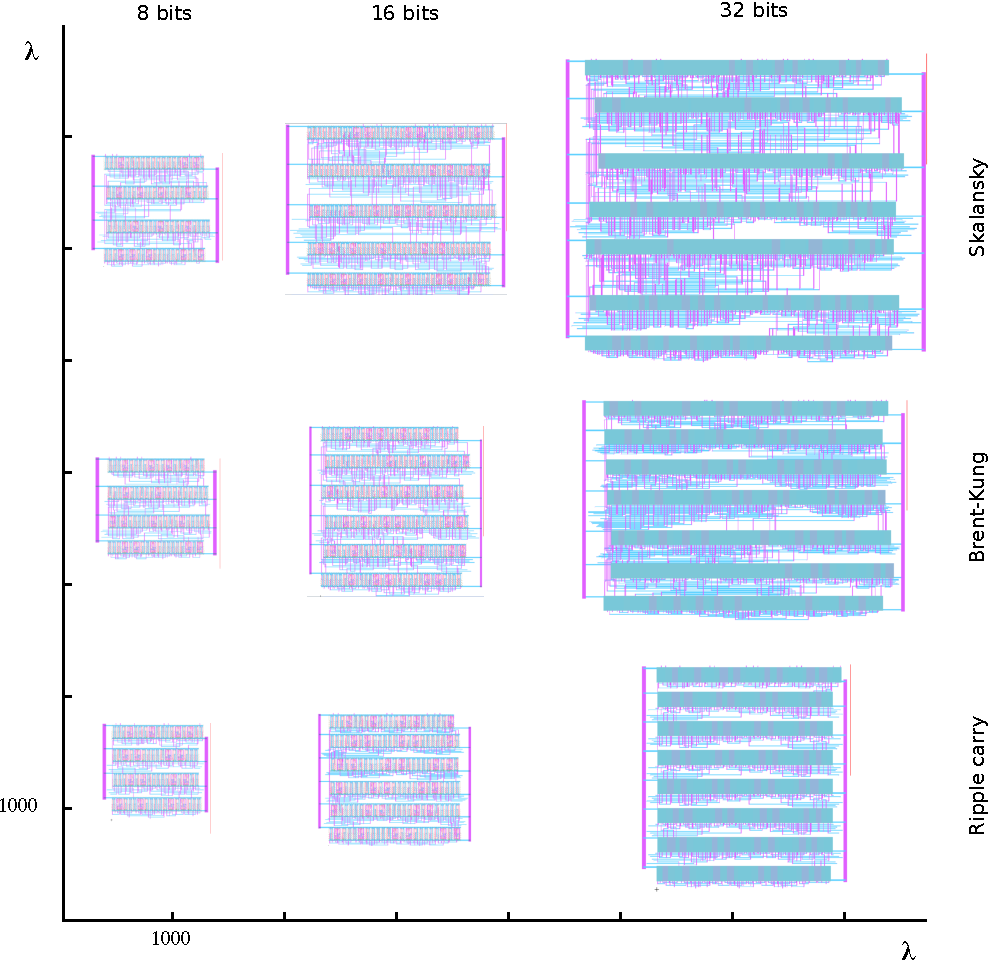
\includegraphics[scale=0.450]{figuras/layout-disenos.pdf}
  \end{figure}
\end{frame}
%-------------------------------------------------------------

\begin{frame}{Simulaci�n post \emph{layout} para calcular performance y potencia}
Realizamos extracci�n de par�sitos del \cursi{layout} y utililizamos un motor de simulaci�n anal�gico tipo SPICE, llamado gnucap.
\end{frame}
%-------------------------------------------------------------
\begin{frame}{Flujo para simulaciones anal�gicas}
 \begin{figure}[h]
  \centering
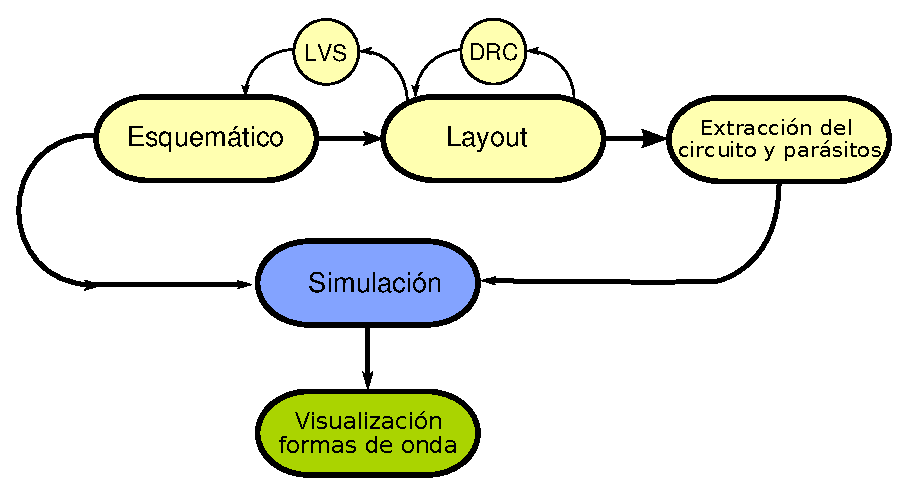
\includegraphics[scale=0.68]{figuras/analog-flow.eps}
\label{fig:aflow}
%\vspace{-10pt}
\end{figure}
\end{frame}
%%-------------------------------------------------------------
\begin{frame}{Retardo de propagaci�n}
  \alert{Definici�n:}

Retardo de propagaci�n de un inversor:
\begin{figure}[h]
\centering
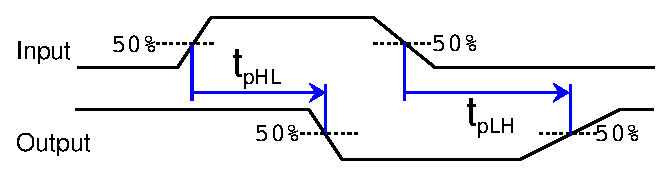
\includegraphics[scale=0.65]{figuras/tiempo_retardo_tpHL-tpLH.eps}
  \label{fig:propagationDelay}
\end{figure}

Se define usualmente el retardo de propagaci�n como:

$$ t_p = \frac{t_{pLH} + t_{pHL}}{2} $$

\end{frame}
%-------------------------------------------------------------
\begin{frame}{Simulaci�n post \emph{layout} para calcular performance}
\begin{figure}
  \centering
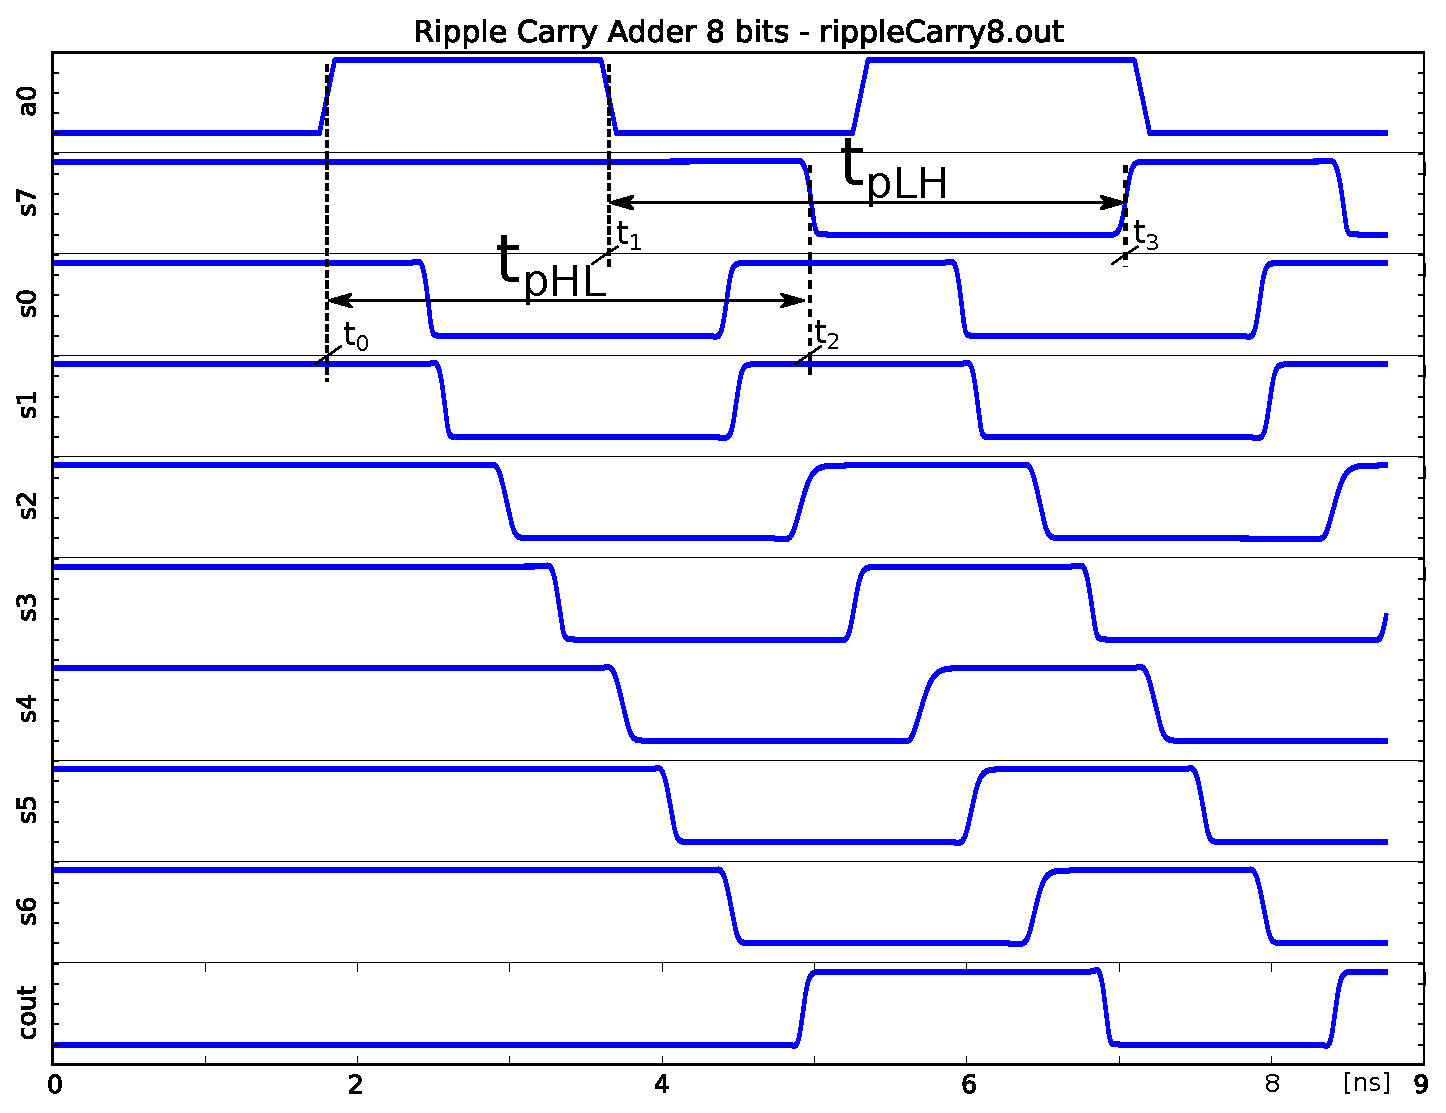
\includegraphics[scale=.36]{figuras/sim_rca8bits_.eps}
\end{figure}
\end{frame}
%-------------------------------------------------------------
\begin{frame}{Simulaci�n post \emph{layout} para calcular performance }
Sumador de 8 bits de \cursi{ripple carry}
\begin{figure}
  \centering
 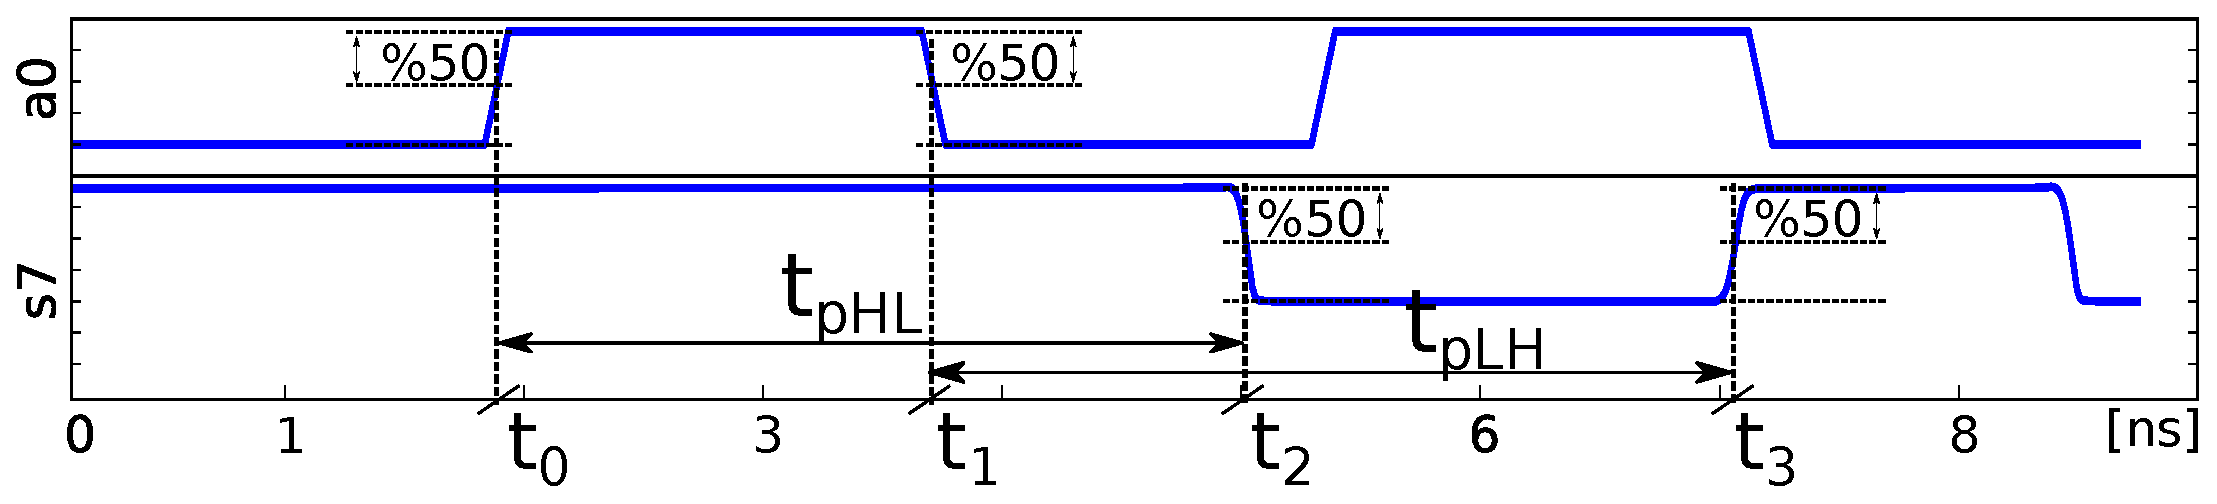
\includegraphics[scale=.29]{figuras/rca8bits_zoom.eps}
\end{figure}

$$t_{pHL} = t_2 - t_0 = 5.01~\ns - 1.8~\ns = 3.21~\ns$$
$$t_{pLH} = t_3 - t_1 = 7.05~\ns - 3.61~\ns = 3.44~\ns$$
$$t_p = \frac{(t_{pHL} + t_{pLH} )}{2} = 3.325~\ns$$
\end{frame}

%-------------------------------------------------------------
\begin{frame}{Potencia promedio disipada}
  \alert{Definici�n:}

La potencia promedio disipada total la podemos calcular si conocemos la corriente instant�nea que brinda la fuente de tensi�n $V_{DD}$, como podemos ver en la ecuaci�n \ref{eq:pv}.
\begin{figure}[h]
\centering
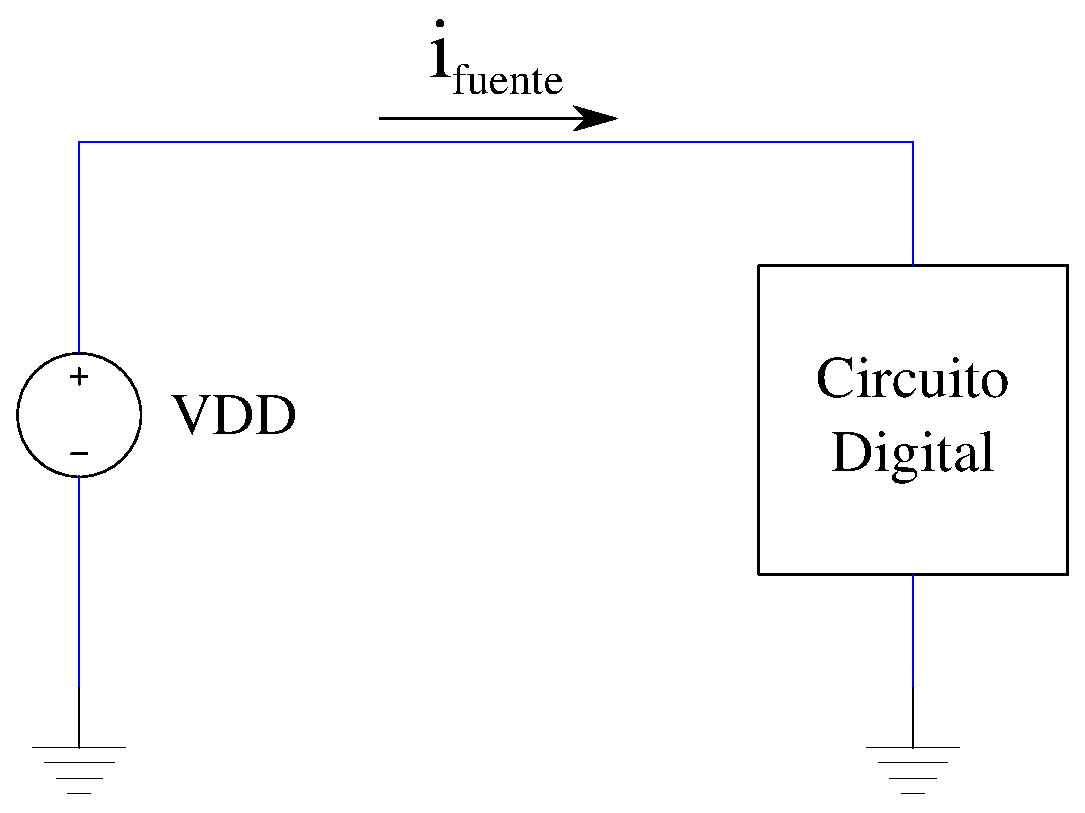
\includegraphics[scale=.21]{figuras/powerSupply.eps}
\end{figure}

\begin{equation}
P_{av} = \frac{1}{\mathrm{T}}\int\limits_0^T p(t)dt = \mathrm{\frac{V_{DD}}{T}}\int\limits_0^T i_{\mathrm{fuente}}(t)\mathrm{d}t 
\label{eq:pv}
\end{equation}
\end{frame}

%-------------------------------------------------------------
\begin{frame}{Simulaci�n de r�gimen transitorio del circuito Ripple Carry 8 bits}
\begin{figure}
  \centering
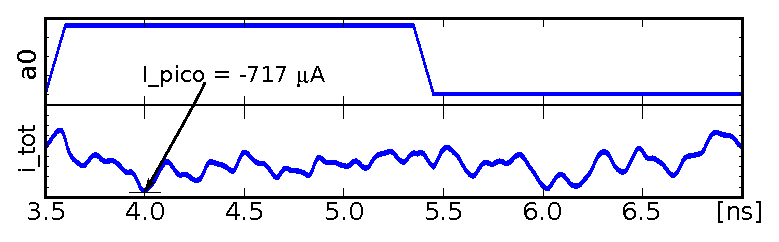
\includegraphics[scale=0.7]{figuras/rca8bits_power.eps}
\end{figure}
El per�odo de integraci�n que elegimos est� determinado por el $t_p$ del circuito, lo que f�sicamente quiere decir: Medimos la potencia del circuito cuando est� funcionando a la mayor velocidad posible. 
\end{frame}

\begin{frame}{Simulaci�n post \emph{layout} para calcular performance y potencia}
  \begin{block}{Simulaci�n post \cursi{layout}}
Realizamos las simulaciones de todas las arquitecturas y de los tres tama�os.
\end{block}
\end{frame}
%

%-------------------------------------------------------------
\begin{frame}{Resultados: Performance}
  \begin{figure}
  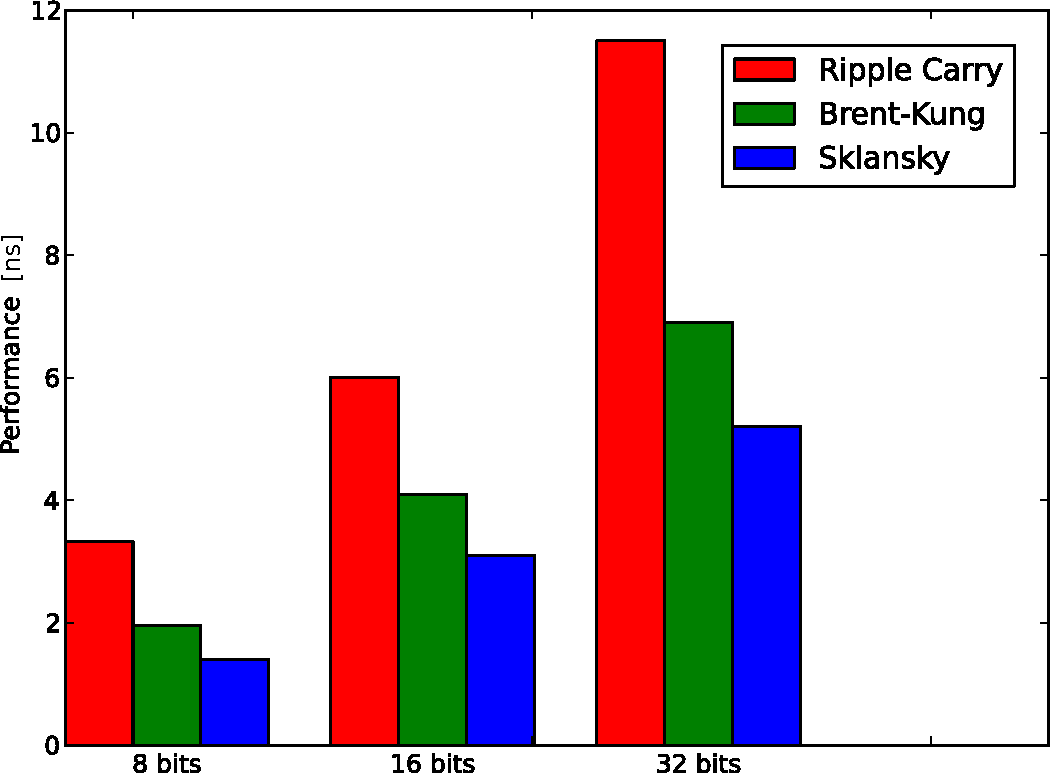
\includegraphics[scale=0.50]{figuras/barra_performance.pdf}
  \end{figure}
  \end{frame}
%-------------------------------------------------------------
\begin{frame}{Resultados: Potencia}
  \begin{figure}
  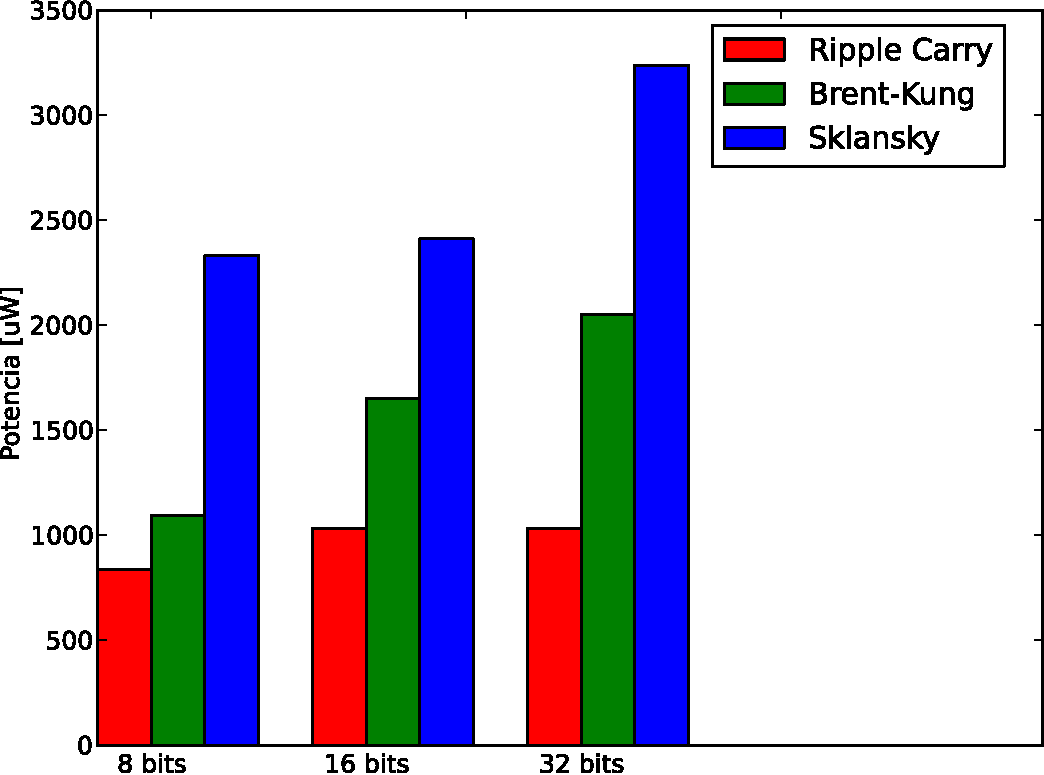
\includegraphics[scale=0.50]{figuras/barra_potencia2.pdf}
  \end{figure}
  \end{frame}
%-------------------------------------------------------------
\begin{frame}{Resumen}
Por lo tanto, hemos logrado un conjunto de sumadores que seg�n los requerimientos de �rea, potencia y performance, podremos elegir la arquitectura m�s adecuada. 

Para todos los tama�os de sumadores,   \begin{block}{Para sumadores de 32 bits}
La mayor velocidad se logra con Sklansky y el mejor compromiso entre velocidad, potencia y �rea con Brent-Kung. 
  \end{block}
  \begin{block}{Para todos los tama�os}
Si la performance no es un problema, un ripple carry es la soluci�n optima de estos tres, ya que ahorra �rea y energ�a.

  \end{block}


  \end{frame}
%-------------------------------------------------------------




%\begin{frame}{Good news about ppp-partitions of genotype matrices.}
%  \begin{theorem}
%    \alert{Optimal ppp-partitions of genotype matrices} can be
%    computed in \alert{polynomial time}. 
%  \end{theorem}
%  \begin{block}{Algorithm}
%    \begin{enumerate}
%    \item Build the following partial order:
%      \begin{itemize}
%      \item Can one column be above the other in a phylogeny?
%      \item Can the columns be the two children of the root of a
%        perfect path phylogeny?
%      \end{itemize}
%    \item Cover the partial order with as few compatible chain pairs 
%      as possible. 
%
%      For this, a maximal matching in a special graph needs to be
%      computed.
%    \end{enumerate}
%  \end{block}
%  \hyperlink{algorithm<1>}{\beamergotobutton{The algorithm in action}}
%  \hypertarget{return}{}
%\end{frame}

\section{Conclusiones}
\begin{frame}
  \frametitle<presentation>{Conclusiones}

  \begin{itemize}
  \item
    Sumadores r�pidos, eficientes o de bajo consumo.
  \end{itemize}
\end{frame}

%\begin{frame}
%  \frametitle<presentation>{Summary}
%
%  \begin{itemize}
%  \item
%    Finding optimal pp-partitions is \alert{intractable}. 
%  \item
%    It is even intractable to find a pp-partition when \alert{just two 
%      noncontiguous  blocks are known to suffice}.
%  \item
%    For perfect \alert{path} phylogenies, optimal partitions can be
%    computed \alert{in polynomial time}.
%  \end{itemize}
%\end{frame}
%

\appendix
\section{Resumen}
\begin{frame}{Resumen}
\end{frame}

%\begin{frame}[label=algorithm]{The algorithm in action.}{Computation of
%    the partial order.}
%  \begin{columns}[t]
%    \column{.4\textwidth}
%    \begin{exampleblock}{Genotype matrix}
%      $G\colon$
%      \begin{tabular}{ccccc}
%        A & B & C & D & E \\\hline
%        2 & 2 & 2 & 2 & 2 \\
%        0 & 1 & 2 & 1 & 0 \\
%        1 & 0 & 0 & 1 & 2 \\
%        0 & 2 & 2 & 0 & 0
%      \end{tabular}
%    \end{exampleblock}
%    \column{.6\textwidth}
%    \begin{exampleblock}{Partial order}
%      \begin{tikzpicture}[node distance=15mm]
%        \tikzstyle{every node}=
%        [%
%          fill=green!50!black!20,%
%          draw=green!50!black,%
%          minimum size=7mm,%
%          circle,%
%          thick%
%        ]
%
%        \node (A) {A};
%        \node (B) [right of=A] {B};
%        \node (C) [below of=B] {C};
%        \node (D) [above of=A] {D};
%        \node (E) [below of=A] {E};
%
%        \path [thick,shorten >=1pt,-stealth'] (A) edge (E)
%                         (B) edge (C)
%                         (D) edge (A)
%                             edge[bend right] (E);
%
%        \uncover<2>{
%        \path [-,blue,thick](A) edge (B)
%                                edge (C)  
%                            (B) edge (E)
%                            (C) edge (E);}
%      \end{tikzpicture}
%
%      Partial order: \tikz[baseline] \draw[thick,-stealth'] (0pt,.5ex)
%      -- (5mm,.5ex); 
%
%      \uncover<2>{\textcolor{blue}{Compatible as children of root:
%          \tikz[baseline] \draw[thick] (0pt,.5ex) -- (5mm,.5ex);}} 
%    \end{exampleblock}
%  \end{columns}  
%\end{frame}
%
%\begin{frame}{The algorithm in action.}{The matching in the special graph.}
%  \begin{columns}[t]
%    \column{.3\textwidth}
%    \begin{exampleblock}{Partial order}
%      \begin{tikzpicture}[node distance=15mm]
%        \tikzstyle{every node}=%
%        [%
%          fill=green!50!black!20,%
%          draw=green!50!black,%
%          minimum size=8mm,%
%          circle,%
%          thick%
%        ]
%
%        \node (A)              {$A$};
%        \node (B) [right of=A] {$B$};
%        \node (C) [below of=B] {$C$};
%        \node (D) [above of=A] {$D$};
%        \node (E) [below of=A] {$E$};
%
%        \path [thick,shorten >=1pt,-stealth'] (A) edge (E)
%                         (B) edge (C)
%                         (D) edge (A)
%                             edge[bend right] (E);
%
%        \path [-,blue,thick](A) edge (B)
%                                edge (C)  
%                            (B) edge (E)
%                            (C) edge (E);
%
%        \only<3->
%        {
%          \path[very thick,shorten >=1pt,-stealth',red] (D) edge (A) (B) edge (C);
%          \path [-,red,very thick](E) edge (B);
%        }
%      \end{tikzpicture}
%    \end{exampleblock}
%    \column{.7\textwidth}
%    \begin{exampleblock}{Matching graph}
%      \begin{tikzpicture}[node distance=15mm]
%        \tikzstyle{every node}=%
%        [%
%          fill=green!50!black!20,%
%          draw=green!50!black,%
%          minimum size=8mm,%
%          circle,%
%          thick,%
%          inner sep=0pt%
%        ]
%
%        \node (A)              {$A$};
%        \node (B) [right of=A] {$B$};
%        \node (C) [below of=B] {$C$};
%        \node (D) [above of=A] {$D$};
%        \node (E) [below of=A] {$E$};
%
%        \begin{scope}[xshift=4.75cm]
%          \node (A')               {$A'$};
%          \node (B') [right of=A'] {$B'$};
%          \node (C') [below of=B'] {$C'$};
%          \node (D') [above of=A'] {$D'$};
%          \node (E') [below of=A'] {$E'$};
%        \end{scope}
%        
%        \path [thick]    (A) edge (E')
%                         (B) edge (C')
%                         (D) edge (A')
%                             edge (E');
%
%        \path [blue,thick](A') edge (B')
%                               edge (C')  
%                          (B') edge (E')
%                          (C') edge (E');
%
%        \only<2->
%        {
%          \path[very thick,red] (D) edge (A')
%                           (B) edge (C')
%                           (B') edge (E');
%        }
%      \end{tikzpicture}
%    \end{exampleblock}
%  \end{columns}
%
%  \medskip
%  \uncover<2->{A \alert{maximal matching} in the matching graph
%    \uncover<3>{induces\\ \alert{perfect path phylogenies}.}}
%
%  \hfill\hyperlink{return}{\beamerreturnbutton{Return}}
%\end{frame}

\end{document}



\pagenumbering{Roman}

\tableofcontents			%%% INCLUYE INDICE AL PRINCIPIO
\listoffigures 
\listoftables
\makeglossary 
\begin{abstracts}
Aca escribo el resumen ...
\end{abstracts}

\chapter{ \textsc{ Introducción } }
\begin{abstract}
En el presente capítulo se describe en rasgos generales el flujo para el diseño de Circuitos Integrados de Aplicación Específica (\emph{ASIC} por su sigla en inglés), y la metodología utilizada para llevar adelante el diseño, implementación y tape out del mismo.
\end{abstract}
\section{Estructura del Proyecto Integrador}

Este proyecto cuenta con 4 partes: Las primeras tres partes:
 
\ref{seleccion_arquitectura}: Selección de la Arquitectura \\
\ref{implementacion_fisica}: Implementación Física \\
\ref{comparacion_resultados}: Comparación de resultados. 

Estas tres partes forman un flujo de trabajo circular e iterativo.

Y finaliza con un resumen de las conclusiones, además de conjunto de anexos técnicos ubicados al final para su consulta.


\section{Planteamiento del problema y motivación}
En la actualidad los microprocesadores, los DSP, los microcontroladores, y otro hardware específico para cálculo computacional son desarrollados en tecnología CMOS submicrónica. El problema planteado es, ¿Cómo hacer para diseñar circuitos integrados en esta tecnología, con herramientas flexibles, libres\footnote{En el sentido que no impongan restricciones de uso, estudio, mejora y distribución.} y accesibles para todo tipo de uso: academico y comercial?.

\section{Objetivo}

El objetivo del trabajo es diseñar un sumador de n-bits, por ser este el elemento central de cualquier tipo de circuito digital de cálculo: Los multiplicadores, los MAC (\emph{multiply-accumulate}), los filtros FIR, etc, que pueda ser enviado a fabricar utilizando
procesos de fabricación CMOS para circuitos integrados. Integrar y documentar un flujo de diseño
de este sistema digital utilizando herramientas de Software Libre, será un subproducto de este
diseño, para lograr la base de conocimiento necesaria en el diseño de circuitos integrados con
tecnología CMOS. Este trabajo además de integrar todos los procesos de diseño de un Circuito
Integrado, pretende facilitar el acceso a las herramientas de diseño de circuitos integrados a los estudiantes de grado.
\section{Plan de Trabajo}


\mainmatter

\part{Diseño Digital}\label{disenio_digital}
% Para compilar la primera vez que se agrega una referencia (/cite):
% Seguir estos cuatro pasos:
% latex Nombre-del-archivo.tex
% bibtex Nombre-del-archivo (sin el .tex)
% latex Nombre-del-archivo.tex
% latex Nombre-del-archivo.tex


% Etiquetas que uso para editar en la próxima iteración:
% FALTA, VER



%Escencia del tema.
%En cada capítulo empezar definiendo.
%En cada capitulo las referencias.

\chapter{ \textsc{ Especificaciones de diseño} }\label{especificaciones}

\section{Introducción}
Los sumadores binarios son utilizados en la adición, la resta, la multiplicación y la división. La velocidad de un sistema de procesamiento de señales, o un sistema de comunicación depende fuertemente de \textbf{estas unidades funcionales\cite{rabaey2003}}. Para cada una de esas operaciones, son necesarios sumadores de distinta cantidad de bits en el mismo diseño. Por lo cual, no se trata solamente de encontrar la arquitectura que para una determinada cantidad de bits logre el mejor compromiso de área, potencia y velocidad. Sino que también esta relacion se mantenga óptima para diferentes tamaños del sumador. 

Por estas razones, precisamos diseñar un sumador de N-dígitos que sea lo más rápido posible, manteniendo una relación de compromiso óptima entre la velocidad, consumo de energía y área del circuito.
Estas características las resumimos en el cuadro \ref{cuadro:especifaciones}.
\begin{savenotes}
\begin{table}[h]
\centering
\begin{tabular}{@{}ll@{}}
\toprule
\textbf{Parámetro}  & \textbf{Especificación} \\ \midrule
Sumandos & Dos\footnote{Dejamos de lado las arquitecturas que implementan la suma de 3 o mas operandos, como pueden ser los sumadores Carry Save Adders} \\	
Cantidad de Dígitos & Parametrizable \\
Proceso de fabricación  & Disponible por medio de MOSIS\footnote{MOSIS es un servicio que permite la fabricación de Circuitos Integrados a muy bajo costo, por medio de obleas multiproyecto que pueden contener muchos diseños de distintos clientes} \\ 
Retardo de propagación  & Lo mas bajo posible                 \\
Potencia total disipada & Tan bajo como sea posible                 \\
Área del Circuito       & La menor posible                \\ \bottomrule
\end{tabular}
\caption{Especificaciones de diseño para el sumador binario}
\label{cuadro:especifaciones}
\end{table}
\end{savenotes}


\section{Métricas de calidad}
Definiremos las métricas que nos permitan dar cuenta de la calidad del diseño.
\subsection{Performance}

El término performance puede representar distintas métricas, según desde qué perpectiva se esté realizando el análisis. Pero si nos enfocamos puramente en el diseño, la performance se define usualmente\cite{rabaey2003} como la duración del período del clock (o su frecuencia). El valor mínimo de período de clock que pueda ser usado para una tecnología y un diseño dado, está definido por múltiples factores, como el tiempo que le toma a las señales propagarse a través de la lógica (retardo de propagación), el tiempo que lleva entrar y salir los datos de los registros, la incertidumbre de llegada del reloj (\emph{clock uncertainty}). Pero el núcleo de todo análisis de performance reside en la performance de una sola compuerta.

\subsubsection{Retardo de propagación}
El retardo de propagación $t_p$ de una compuerta define cuán rápido responde un circuito a un cambio en su(s) entrada(s). Expresa el retardo experimentado por una señal cuando pasa a través de una compuerta. Medido entre el 50\% del punto de transición de entrada y salida, como mostramos en la figura \ref{fig:propagationDelay}, correspondiente al tiempo de propagación de una compuerta inversora. Ya que el tiempo de propagación es distinto según el flanco de entrada, se definen 2 tiempos de propagación. El $t_{pLH}$ es el tiempo de respuesta de una compuerta  para una transición de la salida desde bajo a alto, mientras que $t_{pHL}$ se refiere a el tiempo para una transición de la salida desde alto a bajo. El retardo de propagación $t_p$ se define como el promedio de estos dos.

$$ t_p = \frac{t_{pLH} + t_{pHL}}{2} $$

\subsubsection{Camino Crítico}
En un circuito digital con varias entradas y salidas, pueden existir mas de un camino desde la entrada hasta la salida. Se suele denominar camíno crítico a aquel camino que tenga el mayor retardo de propagación, ya sea por cantidad de lógica que atraviesa o por las capacidades parásitas de las conexiones. El retardo de propagación de este circuito será el retardo de propagación del camino crítico.


\begin{figure}[h]
\centering
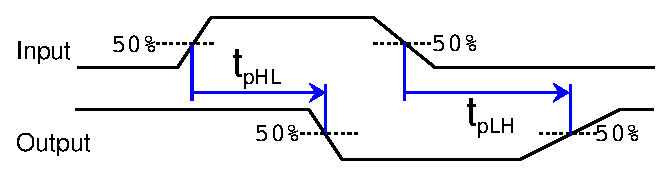
\includegraphics[scale=1.]{figuras/tiempo_retardo_tpHL-tpLH.eps}
  \caption{Retardo de propagación de un inversor}
  \label{fig:propagationDelay}
\end{figure}



\subsubsection{Mínimo retardo de propagación}

Para poder comparar la performance de distintas tecnologías, se busca un circuito que no incluya parámetros como el fan-in o fan-out, que influyen en los tiempos $t_f$, $t_r$ y $t_f$. Por ello, el circuito que es un estándar de facto para medir el tiempo de propagación, es el oscilador anillo (\emph{ring oscillator}), que es un número impar de inversores conectados en serie, con la salida conectada a la entrada. Este circuito oscilla espontaneamente, a una frecuencia de $T = 2 \times t_p \times N$, con $N$ el número de inversores en la cadena. 

Contar con esta métrica nos permitirá tener una referencia del límite inferior impuesto por la tecnología que se esté utilizando. Por ejemplo, tomemos la tecnología TSMC de 180~nm: La frecuencia de un oscilador anillo de 31 etapas es de 377,13~MHz. Es decir que el tiempo de propagación de una celda inversora en esta tecnología es $t_p = 47,8~ps$


%(TODO: Citar DIGITAL DESIGN OF SIGNAL PROCESSING SYSTEMS 5.5.1 )




%FIGURA
%(Multiplicadores, Filtros FIR, usando sumadores)


%Funcionamiento esperado: Se buscará acercarse lo mas posible a la frecuencia máxima de funcionamiento de los circuitos secuenciales para la tecnología CMOS seleccionada, que está caracterizada por la frecuencia de oscilación de un ring oscilator de 31 etapas. Lo
%mismo en cuanto a la especificación de potencia, se utilizará como referencia el número de unidad uW/MHz/gate de ese ring oscilator, que expresa la potencia de un inversor oscilando a la frecuencia máxima.




\subsection{Potencia promedio disipada}
Realizamos el análisis de potencia a lo largo de un período de tiempo $\mathrm{T}$. La potencia promedio disipada total la podemos calcular si conocemos la corriente instantánea que brinda la fuente de tensión $V_{DD}$, como podemos ver en la ecuación \ref{eq:pv}.
\begin{figure}[h]
\centering
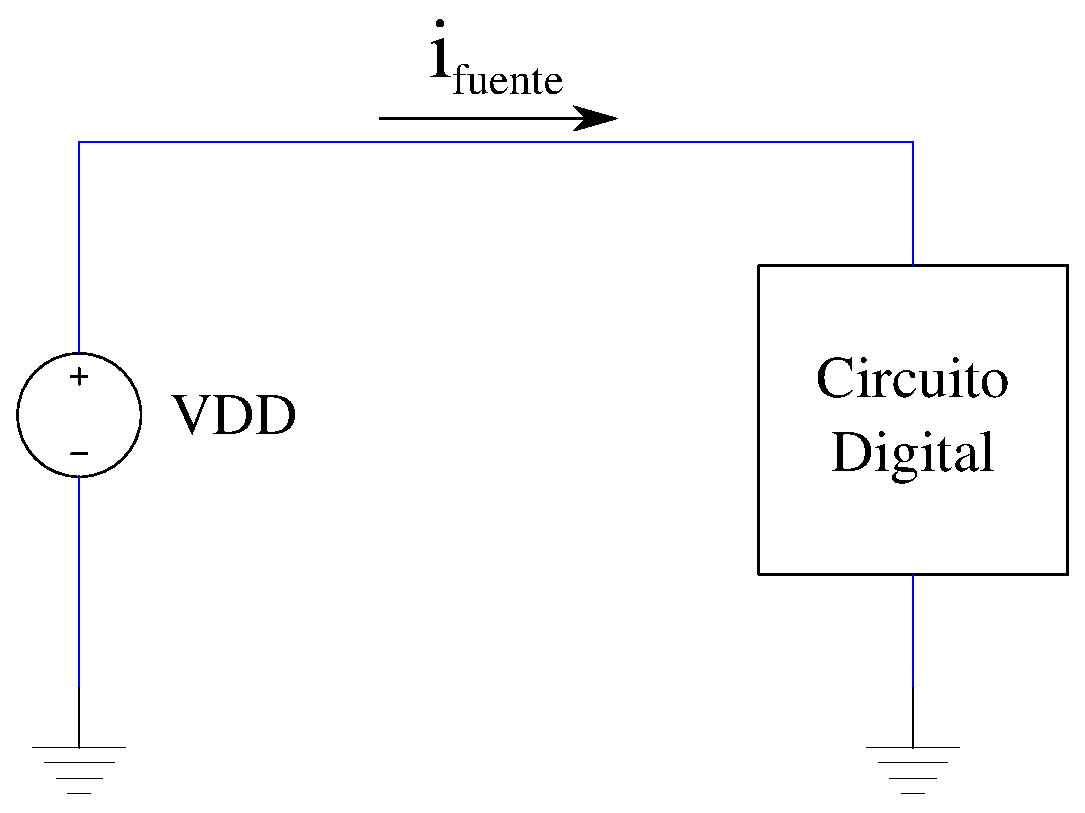
\includegraphics[scale=.5]{figuras/powerSupply.eps}
  \caption{Estimación de Potencia Promedio Disipada }
  \label{fig:powerSupply}
\end{figure}

\begin{equation}
P_{av} = \frac{1}{\mathrm{T}}\int\limits_0^T p(t)dt = \mathrm{\frac{V_{DD}}{T}}\int\limits_0^T i_{\mathrm{fuente}}(t)\mathrm{d}t 
\label{eq:pv}
\end{equation}
El período de tiempo que tomaremos para la integral es el retardo de propagación del camino crítico.

\subsection{Área}
La importancia de minimizar el área de los circuitos radica principalmente en que esta impacta fuertemente en el costo de cada \emph{die}\cite{HennessyPatterson}, ya que el costo es una función que depende de la cuarta potencia del área del circuito\cite{rabaey2003}. Además, los circuitos de menor área tienden a consumir menor energía. 


\subsection{Resumen}
A continuación resumimos en la tabla \ref{cuadro:metricas} las métricas que utilizaremos para la comparación de las distintas arquitecturas de sumadores:
\begin{table}[h] 
\centering
\begin{tabular}{@{}ll@{}}
\toprule
\textbf{Métrica}  & \textbf{Unidades} \\ \midrule
Retardo de propagación & [ns] \\	
Potencia promedio disipada & [mW] \\
Área de circuito  & [$\mu\textrm{m}^2$] \\ \bottomrule
\end{tabular}
\caption{Métricas de comparación}
\label{cuadro:metricas}
\end{table}




%Quality Metrics of a Digital Design
%Área 
%cost of die = f(die area)^4



%Background:
%Power consumption on cmos
%Dynamic Power, Static Power
%Delay in CMOS



%Glosario:

%Chip
%A tiny, thin square or rectangle that contains integrated
%electronic circuitry. Die are built in batches on wafers
%of silicon. A chip is a packaged die. Chips are also called
%processors and microprocessors. Microprocessors are the
%brains of computers, servers, communications products,
%and other digital devices

%Die: Alternate name for a chip, usually before it is packaged.
%See also Chip


%Wafer
%A thin silicon disc sliced from a cylindrical ingot. Used as
%the base material for building integrated circuits.

% Para compilar la primera vez que se agrega una referencia (/cite):
% Seguir estos cuatro pasos:
% latex Nombre-del-archivo.tex
% bibtex Nombre-del-archivo (sin el .tex)
% latex Nombre-del-archivo.tex
% latex Nombre-del-archivo.tex


% Etiquetas que uso para editar en la próxima iteración:
% FALTA, VER


\chapter{ \textsc{ Sumadores } }\label{diseñoDigital}
	
\section{Introducción}
Tal como mencionamos en la sección \ref{sec:intro_esp} (pág. \pageref{sec:intro_esp}), nuestro objetivo es implementar un sumador binario de $n$ bits, manteniendo la mejor relación de compromiso entre performance, potencia y área según crece \(n\).


% Selección de la Arquitectura 
\subsection{Selección de la arquitectura}\label{sec:selección_arquitectura}

Se puede afirmar que los sumadores llamados (según la bibliografía en inglés) como \emph{parallel prefix adders}\footnote{Nosotros los nombraremos como \cursi{sumadores de prefijo paralelo}.} son los mejores con respecto al producto potencia-retardo\footnote{Cuando decimos retardo, nos referimos al retardo de propagación máximo de un circuito, nuestra métrica elegida para caracterizar la performance.}.  Estos sumadores se clasifican dentro de un mismo tipo, porque reducen el problema de calcular las señales de acarreo como el \textbf{problema de cálculo de prefijo}\footnote{En \ref{subsec:prefixProblem} definimos precisamente el problema.}. A su vez, son implementaciones particulares de los sumadores  conocidos como \emph{carry look-ahead adders}, ya que todos se basan en el cálculo en paralelo de los acarreos.
\subsubsection{\emph{Sumadores de prefijo paralelo}}
Brent-Kung\cite{brent-kung}, Sklansky\cite{sklansky}, Kogge-Stone \cite{kogge-stone}, Ladner-Fisher\cite{ladner-fischer}, Hans-Carlson\cite{kogge-stone} y Knowles\cite{knowles} son implementaciones de este tipo de sumadores, que se diferencian cada uno por minimizar alguna relación de compromiso, en el espacio de diseño para el retardo, área y potencia\cite{Sugla-Carlson} del circuito.

Si tenemos en cuenta el área utilizada por estos circuitos, no podemos asegurar que una de estas se clasifique globalmente como la mejor, ya que algunas implementaciones favorecen una métrica a costa de la otra. Citamos un estudio que presenta los siguientes resultados de la figuras \ref{retardo-bits} y \ref{area-bits} de un estudio comparativo \cite{estrada-gimenez} para tecnología CMOS 0.13~\microm.

\subsubsection{Arquitecturas a implementar}
De estas arquitecturas mencionadas, vamos a implementar un sumador rápido basado en la idea original de Sklansky\cite{sklansky} publicado en 1960. También vamos a implementar una arquitectura que busca la mejor relación entre interconexiones y cantidad de compuertas utilizadas, a costa de un pequeño aumento en la cantidad de etapas, conocido como sumador de Brent-Kung\cite{brent-kung}. Además, implementaremos el sumador de ripple carry para utilizarlo de referencia comparativa.


\begin{figure}[h]
  \centering
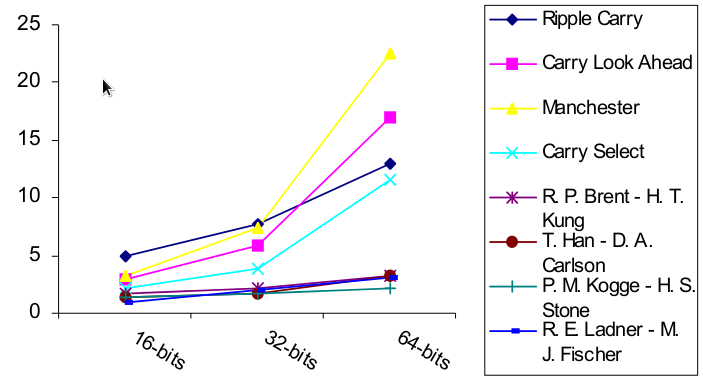
\includegraphics[scale=0.49]{figuras/retardo-bits.png}
\vspace{-5pt}
  \caption{Retardo respecto al tamaño de los operandos}
  \label{retardo-bits}
\vspace{-5pt}
\end{figure}


\begin{figure}[h]
  \centering
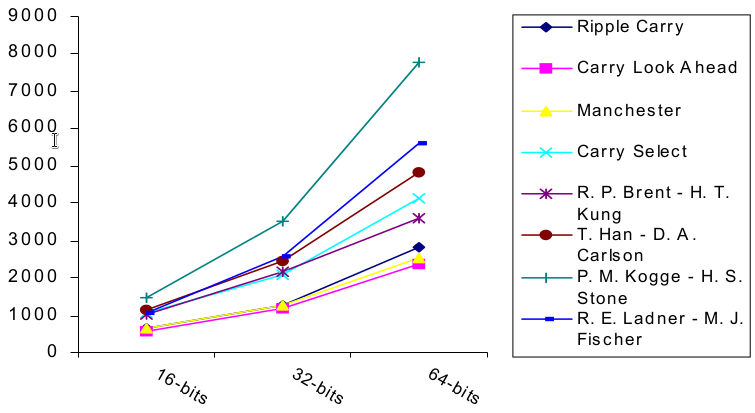
\includegraphics[scale=0.44]{figuras/area-bits.png}
\vspace{-1pt}
  \caption{Área respecto al tamaño de los operandos}
  \label{area-bits}
\vspace{-15pt}
\end{figure}

\begin{table}[h]
\centering
\begin{tabular}{|l|l|l|}
\hline
\multicolumn{1}{|c|}{\textbf{Arquitectura}} & \multicolumn{1}{c|}{\textbf{Retardo Máx.   }} & \multicolumn{1}{c|}{\textbf{Área}} \\ \hline
Ripple Carry  & \(O(n)\) & \(O(n)\) \\ \hline
Carry Look-Ahead  & \(O(\log_2(n))\) & \(O(n\log_2(n))\) \\ \hline
Ladner-Fisher &\( O(\log_2(n))\) & \(O(n\log_2(n))   \) \\ \hline
Sklansky &\( O(\log_2(n))\) & \(O(n\log_2(n))\) \\ \hline
Kogge-Stone & \( O(\log_2(n))\) & \(O(n\log_2n)\)\\ \hline
%Han-Carlson & \( O(\log_2(n))\) &... \\ \hline % Lo quito ya que no encuentro la función de complejidad de área.
Brent-Kung & $O(\log_2(n))$ & \(O(n)\) \\ \hline
\end{tabular}
\caption{Resumen de las funciones de retardo y área de algunos sumadores}\label{tabla:sumadores}
\end{table}

% BKA  Cantidad de operadores (2*n)-2-log_2(n)
% KSA  # de operadores n*log_2(n)-n+1


Resumimos en la tabla \ref{tabla:sumadores} las características y diferencias entre los distintos sumadores\cite{6120598}. Incluimos al \textbf{ripple carry}, por ser la implementación más simple, y al \textbf{carry look-ahead} por ser el sumador que propone el cálculo en paralelo de los acarreos para disminuir logarítmicamente el tiempo de retardo.

%Agregar las referencias a los papers si se puede

%Para justificar la tabla de arriba, vemos los siguientes dos papers:

%"A unified Adder Design" - Wang, Parhi.

%CARACTERIZACIÓN DE SUMADORES EN TECNOLOGÍAS FUERTEMENTE SUBMICRÓNICAS -  Adrián Estrada, Carlos J. Jiménez, Manuel Valencia



\section{Fundamentos teóricos de la suma}
A los fines de poder implementar estos sumadores, desarrollaremos las ecuaciones que nos permitan llegar a la descripción del \cursi{hardware}.

\subsection{Semisumador y sumador completo}
\subsubsection{Semisumador}
El {\bf Semisumador} (Half-adder) recibe 2 bits de entradas \(a\) y \(b\) y produce un bit de suma \(s\) y un bit de acarreo \(c\).

\begin{subequations}
\begin{align}
s &= a \oplus b\\
c &= ab
\end{align}
\end{subequations}

\subsubsection{Sumador Completo}
Luego definimos un Sumador Completo de un bit, o Full Adder:
\begin{center}
\begin{tabular}{lll}
Entradas: & Bits de operandos \(a\) , \(b\) y carry-in \(c_{in}\) & (o \(a_i, b_i, c_i\) para la etapa \(i\)) \\
Salidas: & Suma \(s\) y carry-out \(c_{out}\) & (o \(s_i\) y \(c_{i+1}\) para la etapa \(i\)) \\
\end{tabular}
\end{center}

\begin{subequations}
\begin{align}
s &= a\oplus b \oplus c_{in}
\label{s}
\\
c_{out}&= a b + a c_{in} + b c_{in}
\label{c}
\end{align}
\end{subequations}
%\(c_{out}= (a\wedge b )\vee (a \wedge c_{in}) \vee (b\wedge c_{in})\)

Podemos construir un {\bf sumador completo} (full-adder) combinando las ecuaciones del sumador y semisumador, como vemos en la figura \ref{fig:fulladder}:

\vspace{-1pt}

\begin{figure}[h]
  \centering
\hspace{-23pt}
\begin{subfigure}[b]{0.3\textwidth}
                \centering
                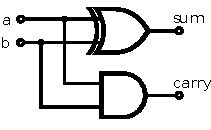
\includegraphics[width=\textwidth]{figuras/halfadd_schem.pdf}
                \caption{Semisumador}
                \label{fig:halfadder}
        \end{subfigure}
\begin{subfigure}[b]{0.5\textwidth}
                \centering
                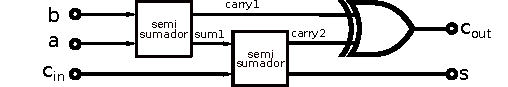
\includegraphics[scale=1.3]{figuras/fullAdd_schem.pdf}
                \caption{Sumador completo}
                \label{fig:fulladder}
        \end{subfigure}

  \caption{Bit adders}\label{fig:bitadders}

\end{figure}

\vspace{0.5cm}

%\section{Selección de la arquitectura del sumador}
%Proponemos el uso de Celdas estándard CMOS (Complementary Metal Oxide Silicon) para la implementación\footnote{Para ver otras posibilidades de implementación lógica, ver (FALTA CITA) RABAEY}. El carácter de nuestro flujo de diseño así lo requiere, ya que se utilizarán herramientas de síntesis de circuitos digitales basadas en celdas estándars. Quedan entonces descartadas las implementaciones utilizando transmition gates, lógica dinámica u otro tipo de implementacion lógica.

\subsubsection{Ripple Carry Adder}

Definimos el sumador Ripple Carry Adder (RCA), utilizando \(n\) sumadores completos para sumar 2 operandos de \(n\) bits. El sumador de \(n\) bits produce una salida de \(n\) bits y una salida de acarreo \(c_{out}\).

Este sumador se implementa conectando como muestra la figura \ref{fig:RCA} el bloque \verb.fullAdd. (Sumador Completo). El camino crítico de la señal se determina considerando el peor camino de propagación de la señal.  

%\vspace{-1pt}
\begin{figure}[h]
  \centering
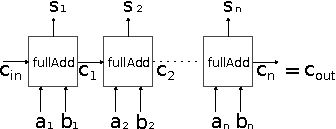
\includegraphics[scale=1.5]{figuras/binnaryAdder.pdf}
  \caption{Ripple Carry Adder}
  \label{fig:RCA}
\end{figure}

El retardo del camino crítico de un sumador de $n$ bits es:

\begin{equation}
T_{RCA} = (n-1)T_m+ T_{FA}
\end{equation}

Siendo $T_m$ el retardo del circuito de generación del acarreo de un sumador completo y $T_{FA}$ el retardo de un sumador completo. Es decir, el retardo es proporcional al tamaño de los operandos.

%\cite{estrada-gimenez}
%Comenzamos con el RCA (Ripple Carry Adder), que tiene un área O(n) y un retardo de compuerta (Delay) de O(n).
%Luego tenemos al CLA (Carry Look-Ahead Adder) con un área de O(n*log(n)) y un delay de O(log(n)).
%Carry Skip Adder(CSA)
%Carry Increment Adder (CIA) Área O(n) y Delay O (nl + 2/ l +1 )  
%Carry Select Adder (CSelA)Área O(n) y Delay O (nl + 2/ l +1 ) 
 
% El delay de un RCA está en pag. 77 de Computer Arithmetic de Behrooz Parhami

\subsection{Sumadores \cursi{carry lookahead}}

La clave para sumar rápido es plantear el problema de la suma como el problema de generar las señales de acarreo en el menor tiempo posible; eso queda evidenciado al interpretar la ecuación \ref{s_i}. Por lo tanto, el objetivo será lograr un bloque generador de las señales de acarreo de baja latencia\cite{arithmeticComputer}.
%Pag. 85 - Section 5.6 (ver como se cita en latex la página)

Ya que una vez que el acarreo en la posición \(i\) es conocido, se puede calcular la suma como:
\begin{equation}\label{s_i}
s_i = a_i \oplus b_i\oplus c_i
\end{equation}

Con respecto al acarreo, lo importante es si en una posición dada el acarreo se \emph{genera} ó se \emph{propaga}. Con las siguientes ecuaciones lógicas podemos definir esas señales:
%

%\vee es el OR
%\wedge es el AND
%\oplus es el XOR
%$$a_i=\lnot{a_i}\wedge\lnot{b_i}=\lnot{(a_i \vee b_i)}$$
$$g_i=a_ib_i$$
$$p_i=a_i \oplus b_i$$


Asumiendo que estas señales se han calculado y están disponibles, podemos calcular recursivamente el acarreo de la siguiente forma:
\begin{equation}
%c_{i+1}=g_i\vee (c_i \wedge p_i)
c_{i+1}=g_i + c_i p_i
\end{equation}


\noindent Esto quiere decir que un acarreo entrará en la etapa \(i+1\) si éste se genera en la etapa \(i\), o si entra en la etapa \(i\) y se propaga.

\subsection{Desenrollando la recurrencia del acarreo}
Uno puede desenrollar esta fórmula recursiva del acarreo hasta lograr una función que dependa directamente de los operandos ($a$ y $b$) y del acarreo de entrada $c_{\text{in}}$:
\begin{equation}
\begin{align}
c_i &= g_{i-1} + p_{i-1}c_{i-1}\notag\\
&=g_{i-1}+p_{i-1}(g_{i-2}+p_{i-2}c_{i-2})=g_{i-1}+p_{i-1}g_{i-2}+p_{i-1}p_{i-2}c_{i-2}\notag\\
&=g_{i-1} + p_{i-1}g_{i-2}+p_{i-1}p_{i-2}g_{i-3}+p_{i-1}p_{i-2}p_{i-3}c_{i-3}\notag\\
&=g_{i-1} +p_{i-1}g_{i-2}+p_{i-1}p_{i-2}g_{i-3}+p_{i-1}p_{i-2}p_{i-3}g_{i-4}+p_{i-1}p_{i-2}p_{i-3}p_{i-4}c_{i-4}\label{gyp}	
\end{align}
\end{equation}

El proceso se repite hasta que el último término contenga $c_0 = c_{\text{in}}$. Podemos computar todos los acarreos en un sumador de $k$-bit directamente con las señales auxiliares ($g_i,p_i$) y $c_{\text{in}}$, utilizando compuertas lógicas AND-OR con un fan-in máximo de $k+1$. Para $k=4$, tenemos:
\begin{equation}
\begin{align}
c_4 &=g_{3} +p_{3}g_{2}+p_{3}p_{2}g_{1}+p_{3}p_{2}p_{1}g_{0}+p_{3}p_{2}p_{1}p_{0}c_{0}\\
c_3 &=g_{2} +p_{2}g_{1}+p_{2}p_{1}g_{0}+p_2p_1p_0c_0\\
c_2 &=g_{1} +p_{1}g_{0}+p_{1}p_{0}c_{0}\\
c_1 &=g_0+p_0c_0\\
\label{carries}	
\end{align}
\end{equation}	
Aquí, $c_4$ y $c_0$ son los $c_{\text{out}}$ y $c_{\text{in}}$ respectivamente de un sumador de 4-bits. Podemos usar un bloque de acarreo basado en estas ecuaciones, y usando compuertas AND de 2 entradas para $g_i$ y compuertas XOR de 2 entradas para $p_i$ y los bits de suma, construimos un sumador de 4-bits. Este sumador es conocido como \emph{carry lookahead adder (CLA)}. Notar que como $c_4$ no se usa para calcular la suma, no es necesario aplicar la ecuación \ref{carries} y lo podemos obtener usando una ecuación más simple, sin tener casi un deterioro en velocidad:
\begin{equation}
\begin{align}
c_4 = g_3 + c_3p_3 \notag
\end{align}
\end{equation}
La red de acarreo que resulta de estas ecuaciones la podemos ver en la figura \ref{cla4bits}.
\begin{figure}[h]
  \centering
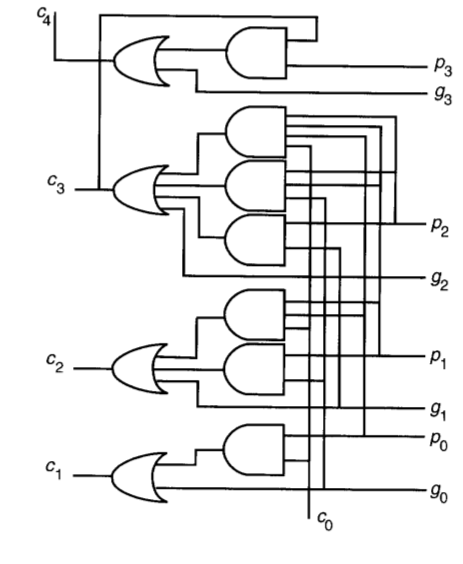
\includegraphics[scale=0.43]{figuras/fulladder4bitcla.png}
\vspace{-1pt}
  \caption{CLA 4-bits}
  \label{cla4bits}
\vspace{-15pt}
\end{figure}

Si observamos las ecuaciones \ref{carries}, vemos que el retardo de esta red será el retardo $T_{AND_n}$ de la mayor celda AND, mas el retardo $T_{OR_n}$ de la operación OR de $n$ entradas. Esto es un inconveniente, ya que según aumenta el fan-in también aumenta el retardo. El retardo de un sumador construido con esta red tendrá también el retardo $T_p$ del cálculo de $p$ mas el retardo de un sumador completo.
\begin{equation}
T_{CLA} = T_p + T_{AND_n} + T_{OR_n} + T_{FA}
\end{equation}

Se pueden realizar por medio de árboles binarios una reducción a celdas con un fan-in de dos (por ejemplo), pero agregando una etapa por cada reducción, en ese caso el retardo en este circuito sería en función del $\log_2 n$.


% INTERESANTE: Clock periods in contemporary microprocessors are rather short; they are shorter than 10 times the delay of a full-adder.

\subsection{Sumadores de Prefijo Paralelos (\emph{Parallel Prefix Adders})}
En la sección anterior vimos como desarrollar ecuaciones que nos permiten obtener las señales de acarreo a partir de las señales auxiliares, para poder calcular la suma del bit $n$, sin esperar a que el acarreo del bit $n-1$ sea computado. Aunque esta solución tal cuál como la presentamos deja de ser aplicable según aumenta $n$, nos permite abordar \textbf{el problema del cálculo de los acarreos como un problema de prefijo paralelo}.
\subsubsection{Problema de prefijo paralelo (\emph{parallel prefix problem})}\label{subsec:prefixProblem}
El problema de prefijo paralelo es:

\begin{equation}
\begin{align}
\text{Dado:}\\
 & \text{Entradas:} x_0,x_1,\dotsc,x_{k-1} \\
 & \text{Un operador + asociativo}\\ 
\text{Computar}:&x_0 \nonumber \\
&x_0+x_1 \nonumber \\ 
&x_0+x_1+x_2+ \nonumber \\ 
&\vdots \nonumber \\ 
&x_0+x_1+x_2+\dotsb+x_{k-1} \nonumber
\end{align}
\end{equation}

\subsubsection{Cómputo del acarreo como un problema de prefijo paralelo}
Pensemos la ecuación \ref{gyp} de la siguiente forma, asumiendo que $c_0=c_\text{in}$ viene desde otro bloque:
\begin{equation}
\begin{align}
g_{[i,i+3]} &= g_{i+3}+g_{i+2}p_{i+3}+g_{i+1}p_{i+2}p_{i+3}+g_{i}p_{i+1}p_{i+2}p_{i+3}\nonumber\\
p_{[i,i+3]} &= p_{i}p_{i+1}p_{i+2}p_{i+3}\nonumber
\end{align}
\end{equation}

Podemos interpretar estas ecuaciones de la siguiente forma: las cuatro posiciones de bits propagan colectivamente un acarreo $c_\text{in}$ si y solo sí cada una de las posiciones propaga; y el bloque gener	a un acarreo si en la posición $i+3$ se genera uno, o se podrouce en la posición $i+2$ y es propagado por la posición $i+3$, etc.

Con este procedimiento podemos llegar a expresar una generalización muy importante, para bloques adyacentes que se superponen $[i_1,j_i]$ y $[i_0,j_0]$, con $i_0 \leq i_1 - 1 \leq j_0 < j_i $:
\begin{equation}
\begin{align}
g_{[i_0,j_1]} &= g_{[i_1,j_1]}+g_{[i_0,j_0]}p_{[i_1,j_1]} \nonumber\\
p_{[i_0,i_1]} &= p_{[i_0,j_0]}p_{[i_1,j_1]}\nonumber
\end{align}
\end{equation}
Aquí, $g_{[i_0,j_1]}$ y $p_{[i_0,i_1]}$ son las señales que producimos de 2 bloques adyacentes ($B''$ y $B'$ con sus señales asociadas $(g'',p'')$ y $(g',p')$) que para simplificar la notación nos permite reescribir la anterior ecuación como:
\begin{equation}
\begin{align}
g &= g'' + g'p''\nonumber\\
p &= p'p''\nonumber
\end{align}
\end{equation}
Ahora entonces definimos un operador acarreo $\circ$ para condensar estas operaciones:
\begin{equation}
\begin{align}
(g,p) &= (g'',p'') \circ (g',p') = (g'' + g'p', p'p'')\nonumber
\end{align}
\end{equation}
Este operador es un operador asociativo, y esto se puede demostrar utilizando la propiedad asociativa de los operadores OR y AND. Finalmente, ya tenemos un operador asociativo, y las entradas $(g''',p''')$,$(g'',p'')$,$(g',p'),\ldots$ que nos permiten plantear el problema de la construcción de la red (o bloque) de acarreos, como un \emph{problema de prefijo paralelo}:
\begin{equation}\label{eq:ppProblem}
\begin{align}
\text{Dados:}\\
 & \text{Entradas:} (g_0,p_0),(g_1,p_1),\dotsc,(g_{k-1},p_{k-1}) \\
 & \text{Un operador} \circ \text{asociativo}\\ 
\text{Computar}:\\
(G_0,P_0) = &(g_{[0,0]},p_{[0,0]})\\
(G_1,P_1) = &(g_{[0,0]},p_{[0,0]})\circ(g_{[0,1]},p_{[0,1]})\\
&\vdots  \\
(G_{k-1},P_{k-1}) = &(g_{[0,0]},p_{[0,0]})\circ(g_{[0,1]},p_{[0,1]})\circ \dotsc \circ(g_{[0,k-2]},p_{[0,k-2]})\circ(g_{[0,k-1]},p_{[0,k-1]})
\end{align}
\end{equation}
Retomando la ecuación \ref{s_i} de la suma, y con estas ecuaciones que nos dan las señales propagadas o generadas del acarreo, podemos construir distintos sumadores, que varían en la red de cálculo del acarreo, particularmente en cómo se elija la asociación del operador \cursi{acarreo} (a veces también mencionado como \cursi{operador punto}). La implementación mas básica (y lenta) sería la de ir asociando en serie a este operador, como vemos en la figura \ref{fig:ppserie}. Todos los sumadores de prefijo paralelo se diferencian escencialmente en la forma de asociar.
\begin{figure}[h!]
  \centering
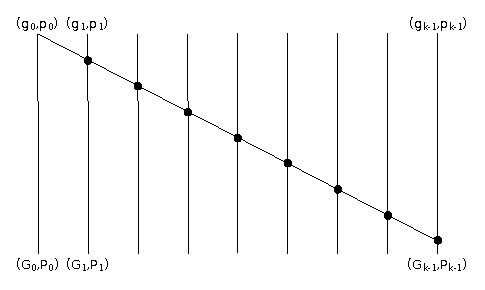
\includegraphics[scale=1.4]{figuras/ppserie.eps}
  \caption{Red de prefijo en serie, una forma gráfica de ver la ecuaciones del cálculo prefijo en \ref{eq:ppProblem}. Notar que cada línea representa dos bits. Los puntos negros representan al operador acarreo.}
\label{fig:ppserie}
%\vspace{-10pt}
\end{figure}
%118 del Parhami " Computer Arithmetic: Algorithms and Hardware Designs."



\subsection {Sumador de Brent-Kung}
Para tener en cuenta el problema de la interconexión entre las compuertas de forma tal que estas sean mínimas y que el área de celdas y de conexión se minimicen, se propone el sumador de Brent-Kung\cite{brent-kung}. Este sumador es una versión que considera el problema de la interconexión entre las compuertas, de una forma que minimice el área, a costa de un aumento en el retardo. Esto se expresa en la función de retardo que es \(2\log_2(n)-2\), a diferencia de los sumadores de Ladner-Fisher\cite{ladner-fischer}, Kugge-Stone\cite{kogge-stone} y Sklansky\cite{sklansky} que en \(\log_2(n)\) etapas calculan todas las señales de acarreo. 


\subsubsection {Operador de Brent-Kung}
El operador $\circ$ se define\footnote{Para respetar la notación de la bibliografía original comenzamos a utilizar la notación lógica con \(\vee\), \(\wedge\) y \(\oplus\) como los operadores booleanos AND, OR y XOR respectivamente} como:
\begin{equation}
(g,p) \circ (\hat{g},\hat{p}) = (g\vee(p\wedge\hat{g}),p\wedge\hat{g})\label{gap}
\end{equation}

\begin{figure}[h!]
  \centering
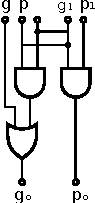
\includegraphics[scale=1.0]{figuras/dotOp_schem.pdf}
%\vspace{-5pt}
  \caption{Operator Punto de Brent-Kung}
  \label{dotOp}
%\vspace{-15pt}
\end{figure}
El operador Punto de Brent-Kung es asociativo, es decir:
$$((a,b) \circ( c,d))\circ (e,f)  = (a,b)\circ((c,d)\circ(e,f))$$
Y por lo tanto podemos ahorrarnos los paréntesis y escribimos:
$$(a,b)\circ(c,d)\circ(e,f)\circ...$$

\subsubsection {Circuito de Generación y Propagación de acarreo}
Ahora necesitamos un circuito que con cada bit de entrada de los operandos \(a\) y \(b\) calcule la señal de acarreo y la de propagación:
$$g_i=a_i \wedge b_i, p_i=a_i\oplus b_i$$
Esas señales se generan en paralelo, dado dos números binarios \(a[n]\) and \(b[n]\) de longitud \(n\).

%vspace{-10pt}

\begin{figure}[h!]
  \centering
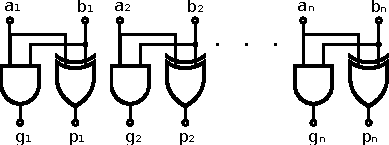
\includegraphics[scale=1]{figuras/gAndPs_schem.pdf}
  \caption{Generación y Propagación del Acarreo}
  \label{gAndPs}
\end{figure}

\subsubsection {Red de Prefijo Paralelo}
\noindent Con la figura \ref{bKung16}, detallamos ahora la red de prefijo paralelo con un fan-out máximo de dos, lo cuál diferencia a el sumador de Brent-Kung de los otros sumadores de prefijo paralelo. La red se realiza con 2 elementos: Los puntos negros son los operadores punto de Brent-Kung de la figura \ref{dotOp} y con buffers (los puntos blancos) que realizan una copia de la señal. Cada cable representa un par de bit \(g_i\),\(p_i\) de la figura \ref{fig:bkungadder}.

\subsubsection {Circuito completo}
Con la red de prefijo paralelo lista, podemos armar el circuito propuesto en el paper de Brent-Kung\cite{brent-kung}. A los fines de la implementación en HDL, mostramos el circuito visto de una forma alternativa en la figura \ref{fig:bkungadder}. Pero aprovechamos la oportunidad para generalizar un poco este resultado. Si retomamos la definición de la suma planteada en la ecuación \ref{s_i}:
$$
s_i = a_i \oplus b_i\oplus c_i
$$
y notamos que en la figura \ref{fig:bkungadder} se calcula $a_i \oplus b_i$, y que con los $G_i$ y los $p_{i-1}$ podemos construir la suma. Por lo tanto, no importa de qué forma se generen estas señales en la red de prefijo paralelo, podemos calcular el valor de $s_i$, como vemos de forma más genérica en la figura \ref{fig:ppadder}.

\begin{figure}[h]
  \centering
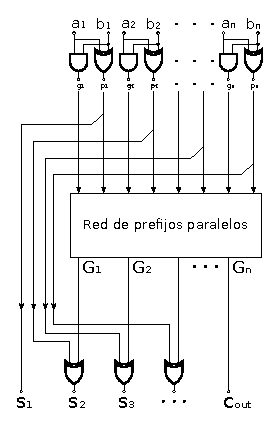
\includegraphics[scale=1.5]{figuras/arquitectura_schem_generico.eps}
  \caption{Sumador de prefijo paralelo}
  \label{fig:ppadder}
\end{figure}

\begin{figure}[h!]
\vspace{-5pt}
  \centering
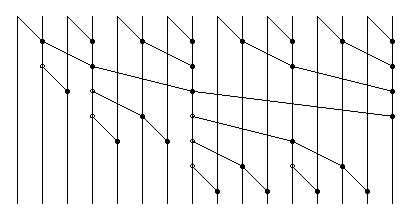
\includegraphics[scale=1.4]{figuras/bKung16.eps}
  \caption{Red de prefijo paralelo para Brent-Kung (ejemplo de 16 bits)}
\label{bKung16}
\vspace{-10pt}
\end{figure}

\begin{figure}[h]
  \centering
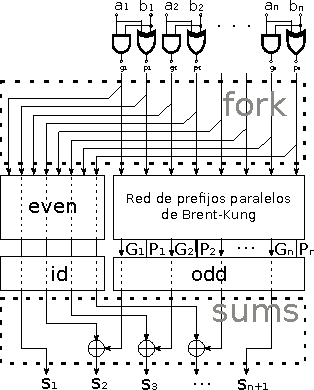
\includegraphics[scale=1.5]{figuras/arquitectura_schem.pdf}
  \caption{Sumador de Brent-Kung}
  \label{fig:bkungadder}
\end{figure}

\subsection{Sumador de Sklansky}\label{subsec:sklansky}
Para realizar este sumador, debemos desarrollar la red de cálculo paralelo de los acarreos, a la forma propuesta por Skalansky. Esta forma se conoce como \emph{divide and conquer}, y la evidenciamos con un ejemplo para sumandos de 16 bits en la figura \ref{fig:sklansky16}. Los puntos negros representan el operador punto (definido anteriormente como el operador de Brent-Kung), notar que tiene menos cantidad de etapas de operaciones (en proporción de $\log_2(n))$) por lo tanto es un sumador más rápido que el de Brent-Kung, pero hay nodos que tienen un fan-out de hasta $\frac{n}{2}$, lo cuál resulta en mayor capacidades parásitas, haciendo más lento el circuito en ese nodo.

\begin{figure}[h!]
\vspace{-5pt}
  \centering
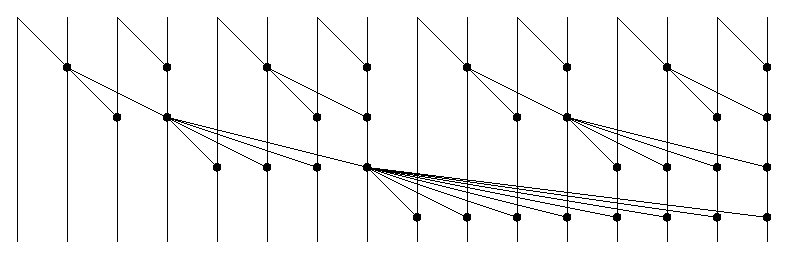
\includegraphics[scale=0.7]{figuras/sklansky16.eps}
  \caption{Red de prefijo paralelo para Sklansky (ejemplo de 16 bits)}
\label{fig:sklansky16}
\vspace{-10pt}
\end{figure}

\chapter{\textsc{Implementación de los circuitos utilizando HDL} }\label{implementaciónHDL}
\section{Introducción}
Utilizamos un lenguaje de descripción de \emph{hardware} para implementar los distintos circuitos que evaluaremos, porque el problema planteado en el capítulo \ref{chap:especificaciones}, requiere que podamos crear un sumador de $n$ bits arbitrario, para lo cuál los HDL son la herramienta mas apropiada. Implementarlos por medio de esquemáticos llevaría mucho tiempo, por eso descartamos esa metodología. En cambio, cuando describimos un circuito con un HDL lo hacemos parametrizando el tamaño del mismo, y a la hora de simularlo o implementarlo físicamente, determinamos su tamaño y generamos automáticamente el circuito. 

\subsection{Breve reseña de HDLs}
VHDL y Verilog son los lenguajes más utilizados y conocidos para el diseño de circuitos integrados. VHDL nace como lenguaje de documentación del comportamiento de los circuitos integrados de aplicación específica (ASIC por su siglas en inglés). El departamento de defensa de Estados Unidos lo desarrolló para poder especificar a sus proveedores, cómo debía comportarse el sistema digital que les encargaba diseñar. Luego, surgio la idea de realizar una simulación lógica a partir de estos archivos VHDL. Lo siguiente fué el desarrollo de herramientas de síntesis lógica a partir de estos archivos, para generar una implementación física del circuito. Con Verilog sucedió algo muy parecido. Por esta historia en común, se puede decir que estos dos lenguajes tienen varias finalidades, siendo la implementación en \emph{hardware} tan sólo una de ellas, es decir, uno puede describir circuitos que no son sintetizables. Por esa razón, y a pesar de ser los más utilizados y conocidos para describir circuitos digitales, no siempre son la mejor alternativa a elegir.

\subsection{Nuevos HDL}\label{subsec:nuevosHDL}
Podemos mencionar al menos 3 lenguajes de descripción de \emph{hardware} que están siendo utilizados para el diseño de circuitos integrados, que nacieron con el objetivo de aprovechar las ventajas de nuevos lenguajes de programación, bajo el paradigma de la programación funcional. Por ejemplo, un circuito que no sea sintetizable, es un error de sintáxis en estos lenguajes. Estos son, \textbf{Lava}\cite{Lava} y \negrita{C$\lambda$aSH}\cite{Clash} basados en \textbf{Haskell}, y \textbf{Chisel}\cite{Chisel}, basado en \textbf{Scala}. 	

Otro lenguaje que debemos mencionar es \textbf{MyHDL}\cite{MyHDL}, un lenguaje basado en Python que brinda muchas ventajas de este lenguaje, que por estar basado en otro paradigma de programación, no lo agrupamos con los dos anteriores. Pero estos cuatro lenguajes nos permiten:

\begin{itemize}
\item Usar un único lenguaje para describir (con distintos niveles de abstracción), simular, verificar e implementar el circuito.
\item Los circuitos se describen en Haskell, Scala o Python (según correspoda), el HDL es simplemente un conjunto de módulos que permiten realizar nuevas tareas relacionadas al diseño de \emph{hardware}, como puede ser crear un netlist VHDL, simulación simbólica, etc. 
\item Generar automáticamente una descripción en VHDL o Verilog, lo cuál nos permite utilizar herramientas de diseño físico que usan este tipo de lenguajes como entrada.
\item Describir circuitos que construimos a partir de subcircuitos, además de la posibilidad de reutilizar fácilmente patrones de conexión.
\end{itemize}

\subsection{Lava}
Podemos elegir arbitrariamente cualquiera de estos lenguajes, ya que ninguno genera un \emph{overhead} en el circuito implementado, pero si en las tareas de aprendizaje del diseñador. Por lo tanto, para este proyecto en particular\footnote{Es un circuito puramente combinacional} se puede elegir el HDL basado en el conocimiento y experiencia de uso en Haskell, Python o Scala.

Para describir el circuito, elegimos Lava. En Lava los circuitos son descriptos como funciones que operan sobre listas, tuplas o sobre circuitos. Esto último se debe a que el lenguaje Haskell permite la definición de funciones de alto orden, es decir podemos definir funciones que su dominio e imagen son funciones. 

Lava es simplemente un conjunto de módulos de Haskell, por lo tanto estamos unificando un conjunto de tareas del diseño digital utilizando un lenguaje de programación de propósito general. Las ventajas de este acercamiento al diseño son varias: 

\begin{itemize}
\item Disponibilidad de todas las librerías existentes en Haskell para ampliar las posibilidades de nuestra herramienta.
\item No se generan \cursi{bugs} típicos de implementar dos veces el mismo circuito en dos lenguajes de programación distintos: El primero en la implementación a nivel de sistema y el otro a nivel de \cursi{hardware}.
\item Se pueden aplicar técnicas de programación propias del lenguaje como \cursi{testing} o \cursi{model checking} con el circuito.
\item Permite manejar otros programas externos, por ejemplo lanzamos \negrita{minisat}\cite{minisat} para verificar formalmente nuestro circuito.  
\end{itemize}


Con la implementación del circuito utilizando este HDL, podemos generar un \negrita{netlist} VHDL, hacer simulación digital, verificación formal de propiedades, y la ventaja de  


\section{Implementación en lenguaje de descripción de hardware}
Ya hemos presentado una descripción esquemática del sumador binario de \(n\) bits en la figura \ref{fig:RCA} y en la \ref{fig:bkungadder}. El objetivo es implementar estos circuito en Lava parametrizando el tamaño \(n\) de los sumandos. 

\subsection{Implementación del sumador de \textbf {ripple carry} en Lava}

\noindent Siguiendo la figura \ref{fig:halfadder}, definiremos el semisumador:
\begin{lstlisting}
halfAdd (a, b) = (s, c)
   where
      s = xor2 (a, b)
      c = and2 (a, b)
\end{lstlisting}
\noindent Para escribir el circuito del sumador completo usamos la figura \ref{fig:fulladder}, nombrando las señales internas y 
escribiendo los subcomponentes de la siguiente forma:
\begin{lstlisting}
fullAdd (cin, (a, b)) = (s, cout)
    where
       (sum1, carry1) = halfAdd (a, b)
       (s   , carry2) = halfAdd (cin, sum1)
       cout           = xor2 (carry2, carry1)
\end{lstlisting}

Por último escribimos la descripción del sumador binario (RCA) de la figura \ref{fig:RCA} de la siguiente forma:

\begin{lstlisting}
rcAdder (carryIn, ([], []))     = ([], carryIn)
rcAdder (carryIn, (a:as, b:bs)) = (sum:sums, carryOut)
   where
      (sum, carry)     = fullAdd (carryIn,(a, b))
      (sums, carryOut) = rcAdder (carry, (as, bs))
\end{lstlisting}

\subsection{Patrones de conexión}
\paragraph{Patrones de conexión estandars.} Los patrones de conexión son funciones de alto orden\footnote{Las funciones de alto orden (\emph{high order functions}) son funciones que toman otras funciones como argumento y devuelven otra función como resultado.} que pueden ser utilizadas para construir circuitos, les llamamos circuitos de alto orden o generadores de circuitos.

\begin{figure}[h]
  \centering
\hspace{-23pt}
%[width=\textwidth]
\begin{subfigure}[b]{0.45\textwidth}
                \centering
                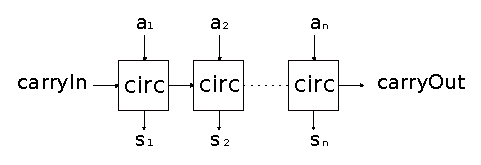
\includegraphics[scale=0.9]{figuras/rowCirc.eps}
                \caption{row}
                \label{fig:rowcirc}
        \end{subfigure}
\begin{subfigure}[b]{0.25\textwidth}
                \centering
                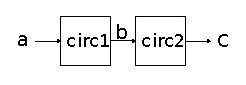
\includegraphics[scale=1]{figuras/serial.eps}
                \caption{serial}
                \label{fig:serial}
        \end{subfigure}
\begin{subfigure}[b]{0.30\textwidth}
                \centering
                \includegraphics[scale=1]{figuras/par.eps}
                \caption{parallel}
                \label{fig:parallel}
        \end{subfigure}
  \caption{Diferentes patrones de conexión de circuitos}\label{fig:pattern}
\end{figure}


Observando la definición de {\footnotesize\verb|rcAdder|} y su topología, podemos generalizar esa estructura de conexión reemplazando el circuito por un parámetro, que en la definición\footnote{Esto es posible dado que Haskell implementa \emph{pattern matching}.} del circuito será una entrada mas. A ese parámetro lo nombramos {\footnotesize\verb|circ|}:

\begin{lstlisting}
row circ (carryIn, ([])) = ([], carryIn)
row circ (carryIn, a:as) = (b:bs, carryOut)
   where
      (b, carry)     = circ (carryIn, a)
      (bs, carryOut) = row circ (carry, as)
\end{lstlisting}
\end{figure}
La función {\footnotesize\verb|row|} toma un circuito {\footnotesize\verb|circ|}, un conjunto de entradas, y las conecta como se muestra en la figura \ref{fig:rowcirc}. Ahora, usando el generador de circuito {\footnotesize\verb|row|}, el sumador binario lo podemos describir mas simplemente asi:
{\footnotesize
\begin{verbatim}
rcAdder' (carry, inps) = row fullAdd (carry, inps)
\end{verbatim}
}
Inclusive para simplificar mas, podemos currificar\footnote{Currificar, es una referencia al lógico Haskell Curry, y hace referencia a la técnica que consiste en transformar una función que utiliza una n-tupla como argumento, en una función que utiliza un único argumento.} la definición:
{\footnotesize
\begin{verbatim}
rcAdder'' = row fullAdd
\end{verbatim}
}

Definir {\footnotesize\verb|rcAdder'|} y {\footnotesize\verb|rcAdder''|} de esa forma es bastante conveniente ya que podemos pensar en término de \emph{generadores de circuitos} en vez de recursión sobre listas.

Ya que hemos visto la ventaja de definir los patrones de conexión, presentamos dos generadores de circuitos que vamos a usar mas tarde:

{\footnotesize
\begin{verbatim}
par cir1 cir2 (a, b) = (c, d)
   where
      c = cir1 a
      d = cir2 b
\end{verbatim}
}
Es muy útil definir una versión mas gráfica de la función {\footnotesize\verb|par|}, si definimos el operador infijo{\footnotesize \verb1-|-1}:
{\footnotesize
\begin{verbatim}
cir1 -|- cir2 = par cir1 cir2 
\end{verbatim}
}
Y por último la conexión serie y su versión con el operador infijo:
{\footnotesize
\begin{verbatim}
serial cir1 cir2 a = c
   where
      b = cir1 a
      c = cir2 b
\end{verbatim}
}
{\footnotesize
\begin{verbatim}
cir1 ->- cir2 = serial cir1 cir2
\end{verbatim}
}
\subsection{Sumador de Brent-Kung}
\subsubsection {Operador de Brent-Kung}
\noindent Comencemos a describir el sumador de Brent-Kung.
En Lava, podemos describir el circuito que implementa la función \ref{gap} siguiendo la figura \ref{dotOp}:

\begin{lstlisting}
dotOp ((g1, p1) ,(g, p)) = (go, po)
   where
      go = or2 (g, and2 (p, g1))
      po = and2 (p, p1)
\end{lstlisting}

\subsubsection {Generación y Propagación del Acarreo}
\noindent En Lava escribimos asi lo que captamos de la figura \ref{gAndPs}:
\lstset{language=Haskell}
{
\begin{lstlisting}
gAndPs ([],[]) = []
gAndPs (a:as, b:bs) = (g,p):gps
   where
      (g, p) = (and2 (a, b),xor2 (a, b))
      gps    = gAndPs (as, bs)
\end{lstlisting}
}


Para ver una explicación con mayor nivel de detalles de cómo construir el circuito, ver el manual de Lava \cite{Lava-tutorial} en conjunto con el paper aqui citado \cite{4638988}


\subsubsection {Red de Prefijos Paralelos para el sumador de Brent-Kung}
\noindent Ahora para describir esta red que usamos en la figura \ref{fig:bkungadder} y mostramos un ejemplo de una red para 16 bits en a figura \ref{bKung16}, nos basamos en un patrón recursivo que propone Sheeran \cite{Shee07} al que le llama \emph{wrap}. En cada paso de la iteración tomamos el resultado anterior (el circuito \(P\)) y le aplicamos el operador punto antes y después de forma intercalada como se puede ver en la figura \ref{sheeranrecurrence}. Esto nos lleva a construir redes como la de la figura \ref{bKung16}.


\begin{figure}[h!]
\centering
 \begin{subfigure}{0.3\textwidth}
    \centering
    \includegraphics[scale=1.5]{figuras/sheeranrecurrence.eps}
    \caption{Patrón de recurrencia}
    \label{sheeranrecurrence}
 \end{subfigure}
 \begin{subfigure}{0.4\textwidth}
    \centering
    \includegraphics[scale 1.4]{figuras/wrapR.eps}
    \caption{Primeras iteraciones de ppNet}
    \label{firstsiter}
 \end{subfigure}
 \caption{Construcción de la red de prefijos paralelos}
\end{figure}


La figura \ref{firstsiter} representa las dos primeras iteraciones del circuito \verb|ppNet|, en el cual la caja de lineas punteada es el caso base de la descripción, los puntos negros son la función \verb|dotOp|. Lo que producimos con esta función recursiva son redes como la de la figura \ref{bKung16}.

A continuación, describimos el circuito \verb|ppNet|, pero antes escribimos las funciones auxiliares \verb|dop|, \verb|unzipl|, \verb|zipl|, \verb|comb|, \verb|posComb|, \verb|miti| y \verb|wrap|, que nos servirán para escribir \verb|ppNet|:


%abss era abs, pero lo renombré xq latex lo resaltaba como una función.
\begin{lstlisting}
dop [a, b] = [a, dotOp(a, b)]
--
unzipl []        = ([],[])
unzipl [a]       = ([a], [])
unzipl (a:b:abss) = (a:as, b:bs)
   where
      (as, bs) = unzipl abss
--
zipl ([], [])     = []
zipl ([a], [])    = []
zipl (a:as, b:bs) = a:b:zipl(as, bs)
--
-- La forma en que hemos escrito las funciones zipl y unzipl 
-- son la clave para lograr una descripcion de un sumador 
-- binario que acepte cualquier cantidad de entradas
--
comb []     = []
comb [a]    = []
comb (a:as) = dop [a, head as] ++ comb (tail as)
--
posComb (a:as)  = a: (comb (init as))++ [last as]
--
miti p = unzipl ->- (id -|- p) ->- zipl
--
wrap p = comb ->- miti p ->- posComb 
\end{lstlisting}

\noindent Luego finalemente, podemos describir {\verb|ppNet|}:

\begin{lstlisting}
ppNet [a]    = []
ppNet [a, b] = dop [a, b]
ppNet as     = wrap ppNet as
\end{lstlisting}


\subsubsection{Circuito top level}
Ahora que ya tenemos construidas todas las partes del sumador, sólo resta juntarlas siguiendo el esquemático de la figura \ref{fig:bkungadder}. Prestar atención a que el circuito \verb|fork| realiza una copia de las señales, el \verb|even| deja pasar los bits pares, \verb|odd| los impares, \verb|id| es la función identidad y \verb|sums| mapea los bits de entrada con la función booleana XOR, salvo el primer y último bit:

\begin{lstlisting}
fork as = (as, as)
--
even as = cs
   where
      (bs,cs) = unzip as
--
odd as = bs
   where
      (bs,cs) = unzip as
-- Unas definiciones mas cortas:
dropP = id -|- odds
dropG = even -|- ppNet
--
sums (a:as,bs) = (a:lastXor (as,init bs),cOut)
   where
      cOut = last bs
--
lastXor (as, bs) = map xor2 cs
   where
      cs = zipp (as, bs)
--
zipp ([],[]) = []

zipp (a:as, b:bs) = c:cs  -- da lo mismo que poner (c:cs)
   where
      c  = (a, b)
      cs = zipp (as, bs)
\end{lstlisting}

\noindent Y el circuito completo es:
\begin{lstlisting}
fastAdd = gAndPs ->- fork ->- dropG ->- dropP ->- sums
\end{lstlisting}

\subsection{Simulación}
En Lava podemos simular el circuito usando la operación {\footnotesize\verb.simulate.}, el circuito y el estado de las entradas, por ejemplo:

{\footnotesize
\begin{verbatim}
simulate fastAdd ([high,low],[low,high])
\end{verbatim}
}

\noindent devuelve:{\footnotesize \verb|([high,high],low)|}. También podemos simular secuencia de entradas con la operación {\footnotesize\verb|simulateSeq|}:

{\footnotesize
\begin{verbatim} 
simulateSeq halfAdd [(low,low),(high,low),(low,high)]
\end{verbatim}
}

\noindent que devuelve {\footnotesize\verb|[(low,low),(high,low),(high,low)]|}

\subsubsection{Simulaciones con números decimales}
Lava nos permite una interfase con números enteros, por si nos interesa simular usando como operandos números enteros. Esto lo logramos si definimos una función como la siguiente, que toma dos enteros y convierte el segundo en un número binario de la cantidad de bits que indica el primero:
\begin{lstlisting}
int2bin 0 num = []

int2bin n num = (bit:bits)
  where
    (bit, num') = numBreak num
     bits      = int2bin (n-1) num'
\end{lstlisting}

\subsubsection{Método de validación del hardware}
Para este diseño en particular, no utilizaremos la simulación como una forma de validar el correcto funcionamiento del circuito, por eso no avanzaremos en las distintas alternativas de simulación que nos permite el sistema, como puede ser la creación de un archivo VCD\footnote{VCD: Value Change Dump es un formato basado en ASCII para loguear señales, que es utilizado por herramietas de simulación lógica. Para visualizarlo podemos utilizar el software GTKWave, de licencia libre.} a partir de vectores de entrada\footnote{Podemos usar una libreria de Haskell llamada \emph{casualmente} \verb.vcd. que nos permite escribir y leer archivos con este formato}.

Justificamos descartar la simulación como método de validación por la simple razón de que sólo simulando todos los posibles estados de las entradas se garantiza el correcto diseño del circuito. Por ejemplo, para un sumador de 64 bits, es necesario simular $2^{128}$ estados.

Para este tipo de sistemas es aplicable la verificación formal automática, que desarrollaremos en el capítulo \ref{verificacion}.

\subsection{Síntesis del \cursi{netlist} VHDL}

Para continuar en nuestro flujo de diseño, precisamos generar el circuito en un lenguaje que nuestra herramienta de \emph{Place and Route} pueda manejar. Para eso Lava nos permite crear un netlist VHDL siguiendo dos pasos, el primero definiendo los nombres de los puertos y el bloque a ser creado:
\begin{lstlisting}
fastAdder n = writeVhdlInputOutputNoClk
              "BrentKungFastAdder" fastAdd
              (varList n "a", varList n "b")
              (varList n "sum", var "cout")
\end{lstlisting}

Y el segundo paso para crear el netlist, debemos especificar el valor real de sumador, por lo tanto valuamos el circuito con en número de bits del sumador y conseguiremos el archivo BrentKungFastAdder.vhl que mostramos en el apéndice \ref{vhdlNetlist}:
\begin{lstlisting}
Main> fastAdder 16
Writing to file "BrentKungFastAdder.vhd" ... Done..
\end{lstlisting}

\noindent Si por alguna razón este netlist lo utilizaramos con una otra herramienta de síntesis, deberemos especificar que no modifique los cables para preservar la estructura de esta red.


% Etiquetas que uso para editar en la próxima iteración:
% FALTA, VER


\chapter{ \textsc{ Verificación Formal } }\label{CONAMURI}

\textsl{ Bla bla bla bla bla bla bla ...\footnote{ Un groso } } 

%\vspace{10mm}

%\textbf{Por Magui Balbuena}\footnote{ Maguiorina (Magui) Balbuena  es dirigente de CONAMURI }

\vspace{10mm}

\section{Propiedades de la suma}
Conmutativa, asociativa, distributiva y existencia del elemento neutro.
\subsection{Herramientas}
\subsubsection{SAT Solvers}
Algo 
\subsubsection{Sumador Completo}
Algo mas


\end{figure}

\vspace{0.5cm}



\section{Selección de la arquitectura del sumador}

Proponemos el uso de Celdas estándard CMOS (Complementary Metal Oxide Silicon) para la implementación\footnote{Para ver otras posibilidades de implementación lógica, ver (FALTA CITA) RABAEY}. El carácter de nuestro flujo de diseño así lo requiere, ya que se utilizarán herramientas de síntesis de circuitos digitales basadas en celdas estándars. Quedan entonces descartadas las implementaciones utilizando transmition gates, lógica dinámica u otro tipo de implementacion lógica.

\subsection{Costo y Retardo de los circuitos combinacionales}
Cada circuito combinacional \(G\) tiene un costo y un retardo. El costo de un circuito combinacional es la suma de los costos de las compuertas en un circuito. Le asignamos un costo unitario a cada compuerta, y el costo del circuito combinacional \(c(G)\) es igual al número de compuertas en el circuito.

El retardo de un circuito combinacional \(d(G)\) se define igual al del retardo de una compuerta. Es el menor tiempo requerido para que las salidas se estabilicen, asumiendo que todas las entradas están estables. Para simplificar el análisis, se le asigna un retardo unitario a cada compuerta.




\part{Diseño Físico}\label{disenio_fisico}
% hacer una macro para \emph{place \& route}

\chapter{Flujo de Diseño Físico}
\section{Introducción}

En este punto convertimos la representación de un circuito (con sus componentes e interconexiones) a una representación en formas geométricas, conocida como \emph{layout}. Dicho en otras palabras, explicaremos (y realizaremos) el proceso que logra transformar una descripción de funciones lógicas a una representación de formas geométricas del circuito integrado, que luego de ser fabricado con las capas correspondientes, nos aseguran que obtendremos los transistores ubicados e interconectados dentro de un chip de silicio, de forma tal que implemente nuestro sistema digital.

El proceso que explicaremos en términos generales, y que podemos ver en contexto en la figura \ref{fig:diseñoFísico}, se realiza iterativamente hasta lograr que el circuito cumpla las especificaciones con el menor costo en potencia disipada y área ocupada.

\begin{figure}[h]
\centering
\includegraphics[scale=0.60]{figuras/DisenioFisico.pdf}
  \caption{Flujo de diseño Físico}
  \label{fig:diseñoFísico}
\end{figure}

\subsection{Etapas del diseño físico}\label{etapasDiseñoFisico}
Generalmente en un flujo de este tipo, partimos desde una descripción estructural del circuito. Esta descripción, comúnmente llamada \emph{netlist}, contiene información sobre qué bloques están presentes, y cómo estos están interconectados.



\begin{description}
\item[Particionado]
Según el tamaño del circuito, será necesario definir particiones del mismo, dividiendo el circuito en dos o mas particiones con fines de acotar la magnitud o dificultad inicial del circuito original, en partes más pequeñas de menor dificultad, si las particiones se realizan correcta e inteligentemente. 
\item[Plano general]
Luego es necesario definir un plano general del circuito (mencionado como \emph{floorplan} en la bibliografía en inglés), que impondrá condiciones físicas mínimas como el área utilizada y la disposición física de las entradas y salidas.
\item[Ubicación]
A continuación, ubicamos en este plano todos los componentes del circuito (conocido como \emph{placement} en la bibliografía en inglés), en una disposición tentativa que nos permita evaluar rápidamente la factibilidad del circuito con las condiciones impuestas por el \emph{floorplan}, por ejemplo si todos los componentes y el conexionado caben dentro del \emph{floorplan}. Depediendo de las herramientas que utilicemos, también se puede tener una estimación sobre la velocidad de las señales. 
\item[Síntesis del árbol de reloj]
Una vez que todos los elementos esten en el plano, si el circuito es secuencial, será necesario realizar una distribución de la señal del reloj para que llegue a todos los registros, de la forma más pareja (en tiempo) posible dentro de un margen de tolerancia determinado. Para ello se agregan \emph{buffers} donde sea necesario. Este proceso se conoce como \gls{cts} en la bibliografía en inglés.
\item[Conexionado]
Por último, se realiza el conexionado de todos los puertos de cada componente, utilizando las capas de metal disponible en la tecnología que se esté utilizando, un ejemplo de este conexionado se puede ver en la figura \ref{fig:routing}. Este proceso se conoce como \emph{routing} en la bibliografía en inglés.
\end{description}

En este punto, se puede realizar la mejor estimación sobre las capacidades y resistores parásitos que representan la interconexión de todo el circuito. Se encuentran los camínos críticos y se realizan las modificaciones necesarias para que el circuito cumpla con la especificaciones de retardo de propagacion máximo. Siempre en cada etapa de este proceso se puede iterar para mejorar el resultado, pero si aún así no logramos la mejora necesaria, debemos volver a iterar sobre una etapa anterior y continuar este flujo, secuencialmente.

El procesos de ubicación de los componentes e interconexionado que acabamos de describir, es muy común que se mencione como \gls{pnr}, por sus siglas en inglés.



\begin{figure}[h]
\centering
\includegraphics[scale=0.7]{figuras/Silicon_chip_3d.png}
  \caption{Representación en tres dimenciones de una celda estándar con 3 capas de metales en color arena, y una capa de silício policristalino en color ladrillo. Azul y rojo son dopado $N^+$ y $P^+$ respectivamente}
  \label{fig:routing}
\end{figure}

\section{Relevamiento, comparación y selección de las herramientas disponibles}\label{sec:herramientasDisponibles}
Para realizar las tareas que describimos en la sección \ref{etapasDiseñoFisico}, será necesario buscar una o varias herramientas de software que se ajusten a los requerimientos del diseño y la tecnología de fabricación\footnote{Se utilizará una tecnología definida por Mead y Conway\cite{mead-conway80}, conocida como  \textbf{SCMOS} (Scalable CMOS).
Esto es un conjunto de capas lógicas junto a sus reglas de diseño, que proveen un proceso casi independiente de la tecnología y dimensión, que sirve para muchos procesos CMOS disponibles a través de MOSIS.} del circuito integrado.

\paragraph{Características esperadas de las herramientas}
\begin{itemize}
\item Desarrollo activo y existencia de una comunidad de usuarios/as y desarrolladores/as que brinden soporte
\item Mayor cantidad de herramientas integradas
\item Flexibilidad para importar y exportar datos. 
\item Disponibilidad de un Kit de diseño para el proceso de la tecnología seleccionada, conocido como \gls{pdk}.
\end{itemize}

\subsection{Relevamiento}
Luego de una inspección de esas características, las herramientas candidatas que cumplen con estas características son:

\begin{description}
\item[Open Circuit Design] Proyecto de software libre que reúne en un único sitio varias herramientas independientes, mencionamos sólo algunas:  \textbf{Magic}: Layout, \gls{drc} y extracción de parásitos; \textbf{Xcircuit}: Entrada de circuitos esquemáticos; \textbf{netgen}: \gls{lvs}; \textbf{IRSIM}: simulador digital a nivel de transistor como llaves ideales, con modelo de retardo simplificado; \negrita{vesta}: herramienta para hacer \gls{sta}; \textbf{Qflow}: entorno para realizar la síntesis digital con celdas estándar, utiliza Yosys\cite{Yosys}; \textbf{graywolf}: programa que realiza el \emph{placement}; \textbf{Qrouter}: programa que realiza el conexionado.

\item[Electric VLSI Design System\cite{Electric}] Es un sistema de automatización de diseño electrónico. Es un entorno integrado muy flexible que permite la descripción del circuito de varias formas (circuitos esquemáticos, \emph{netlist} VHDL y \emph{layout})). Cuenta también con herramientas para hacer \gls{drc}, \gls{lvs} y \gls{pnr}, simulación digital, visualización de formas de ondas, y un generador de \emph{pad frame}\footnote{El \emph{pad frame} es un conjunto de celdas que se ubican en el marco del \emph{die}, para conectar las señales del circuito con el exterior del chip.},entre otras herramientas.

\item[Alliance VLSI CAD System\cite{Alliance}] Alliance es un conjunto de herramientas libres, y celdas estándar para el diseño de VLSI. Incluye un compilador vhdl y un simulador, herramientas de síntesis de lógica, y herramientas de \gls{pnr} automáticas. Brinda un conjunto completo de celdas estándar CMOS escalables.

\end{description}

Es importante mencionar que existen mas herramientas disponibles (y muy útiles), pero al momento de realización de este trabajo, no forman parte de un flujo de diseño que las integre y por ello no son mencionadas aquí. 

\subsection{Comparación}
En la tabla \ref{tabla:Comparativa} resaltamos las ventajas y desventajas de cada herramienta, que nos permitirá hacer una selección en función de las necesidades del proyecto.


%%%%%%%%%%%%%%%%%%%%%%%%%%%%%%%%%%%%%%%%%%%%%%%%%%%%%%%%%%%%%%%%%%%%%%%%%%%%%%%%%%%%
%%%%%%%%%%%%%%%%%%%%%%%%%%%%%%%%%%%%%%%%%%%%%%%%%%%%%%%%%%%%%%%%%%%%%%%%%%%%%%%%%%%%
%
% Tabla comparativa de ventajas y desventajas de las herramientas de diseño físico.
%
%%%%%%%%%%%%%%%%%%%%%%%%%%%%%%%%%%%%%%%%%%%%%%%%%%%%%%%%%%%%%%%%%%%%%%%%%%%%%%%%%%%%
%%%%%%%%%%%%%%%%%%%%%%%%%%%%%%%%%%%%%%%%%%%%%%%%%%%%%%%%%%%%%%%%%%%%%%%%%%%%%%%%%%%%

\begin{center}
    \begin{tabular}{  p{1.5cm}  p{6cm}  p{5cm} }
    \toprule
     & Ventajas & Desventajas  \\  \midrule
%%%% ELECTRIC %%%%%
    \negrita{Electric}
%% Ventajas %%
	& Fácil instalación, acepta Python 
y Java como lenguajes para automatizar el diseño 
o implementar nuevos algoritmos de \gls{pnr}.
Todas las herramientas están integradas.
	Soporta muchos formatos de entrada y salida, 
que nos permite utilizar otras herramientas.
%% Desventajas %%
     & No tiene herramienta para \gls{sta}.
No incluye un compilador lógico, sólo acepta \netlist VHDL
para hacer \gls{pnr}.
\\ \hline

%%%% MAGIC %%%%%
    \negrita{Open Circuit Design}
%% Ventajas %%
	& Para realizar \gls{sta} utiliza el estándar abierto Liberty.
	Extracción de parásitos muy precisa. Permite integración con otras herramientas fácilmente.
%% Desventajas %%
	& Muchos programas para instalar por separado. Díficil de instalar
en otros sistemas operativos no libres.
\\ \hline

%%%% ALLIANCE %%%%%
    \negrita{Alliance} 
%% Ventajas %%	
	& Incluye varias opciones de celdas estándar convenientemente integradas en la herramienta. Tiene todas las herramientas necesarias para un flujo físico completo.
%% Desventajas %%
	& Las herramientas para \gls{sta} y conexionado no tienen una licencia libre. No facilita la integración con otras herramientas externas.
\\ \bottomrule
    \end{tabular}\label{tabla:Comparativa}
\end{center}
%%%%%%%%%%%%%%%%%%%%%%%%%%%%%%%%%%%%%%%%%%%%%%%%%%%%%%%%%%%%%%%%%%%%%%%%%%%%%%%%%%%%
%%%%%%%%%%%%%%%%%%%%%%%%%%%%%%%%%%%%%%%%%%%%%%%%%%%%%%%%%%%%%%%%%%%%%%%%%%%%%%%%%%%%


\subsection{Selección}
La herramienta que seleccionamos es \textbf{Electric}, ya que nos brinda una serie de ventajas comparativas, teniendo en cuenta que nuestro circuito es puramente combinacional y no demanda gran esfuerzo de \gls{pnr} a la herramienta. Podemos resumir :
\begin{itemize}
\item Fácil instalación
\item Curva de aprendizaje suave
\item Cuenta con todas las herramientas necesarias integradas
\end{itemize}
El hecho de que no cuente con un sintetizador lógico, como señalamos en la tabla \ref{tabla:Comparativa}, no tiene importancia para esta selección, ya que uno de los resultados del diseño digital del capítulo \ref{diseñoDigital} es un \emph{netlist} VHDL. Por la naturaleza de la solución propuesta, no deseamos que este resultado sea modificado por alguna optimización lógica, ya que rompería la interconexión original de nuestro circuito. Si quisieramos comparar nuestra implementación del circuito con la implementación automática de la operación suma, entonces tendríamos que pasar a una de las otras herramientas. Pero eso sería un trabajo de comparación de un diseño \emph{custom} con uno automático, que no era el objetivo de este proyecto. 
%Open-Source VLSI CAD Tools: A Comparative Study

\section{Selección del proceso de fabricación}\label{procesoFabricación}
%En la industria del semiconductores bajo el modelo de diseño fuera de la planta de fabricación del chip.

En este punto, es importante mencionar un aspecto de la industria de los semiconductores. En los orígenes, la industria de semicoductores estaba verticalmente integrada. Esto significaba que la misma empresa que diseñaba el producto, también diseñaba las herramientas de software y fabricaba el chip. Pero hace poco mas de 20 años, surge la separación del proceso de diseño y fabricación. Hoy en día existen empresas que se dedican sólamente a desarrollar el producto, otras que se dedican únicamente a desarrollar herramientas de software para el diseño, otras que sólamente se dedican a fabricar los diseños de otras empresas, y también persisten las empresas que realizan todo el proceso (conocidas como \gls{idms}), abriendo las puertas a otras empresas de diseño sin fábrica (conocidas como \emph{fabless}), para evitar la capacidad ociosa instalada y disminuir sus costos.
\subsection{Obleas multiproyectos}
Dentro de este esquema, existe una empresa (MOSIS) que se dedica a recolectar proyectos de diseño que están en etapa de prototipo o de bajo volumen, creando obleas multiproyecto que se envían a fabricar, dividiendo los costos por la cantidad de proyectos que incluye. De esta forma, se logra acceder a la fabricación de circuitos integrados a muy bajo costo. Tiene sus limitaciones en cuanto a tecnologías de fabricación disponibles, cantidades, y tiempo de entrega largos, pero permite que proyectos educativos, de investigación o de baja escala sean económicamente factibles. Es importante mencionar que MOSIS cuenta con un programa especial para las universidades, que permite acceder a ciertos nodos\footnote{Nodo es una forma alternativa de llamar al proceso tecnológico de fabricación que toma como segundo nombre el largo mínimo de canal de un trasistor MOS; por ejemplo: nodo de 180~\nanom ~se refiere al proceso con el cuál se puede fabricar un transistor con un mínimo de 180~\nanom~de ancho de canal.} a muy bajo costo.

Por ello, nuestras opciones serán alguna de las que MOSIS ofrece. En la tabla \ref{tab:procesosDisponibles} vemos una lista que está en constante cambio y actualización, se brinda aquí de modo ilustrativo. Para una lista actualizada visitar https://www.mosis.com/products/fab-processes.

\begin{table}[h]
\centering
\begin{tabular}{@{}lc@{}}
\toprule
Fábrica             & Proceso CMOS \\ \midrule
TSMC                & 28~nm - 180~nm             \\
Globalfoundries     & 14~nm - 180~nm             \\
IBM                 & 32~nm -  250nm            \\
ON Semi             & 0.35~um - 0.7~um           \\
Austria Micro Systems & 180~nm - 0.35~um           \\ \bottomrule
\end{tabular}
\caption{Procesos disponibles por medio de MOSIS}
\label{tab:procesosDisponibles}
\end{table}

De todas estas, elegimos TSMC 180~nm por dos razones: la primera es que cuanto mayor es la dimensión de la tecnología, más simples son las herramientas de software necesarias y más bajo es el costo de fabricación. La segunda, es que con esta tecnología se pueden realizar sistemas de gran complejidad y alta performance\footnote{Claro que cuanto más nueva es la tecnología, los circuitos digitales son más rápidos y disipan menor potencia dinámica. Pero también es cierto que mayores son los tiempos para diseñar, principalmente porque con cada nuevo nodo aparecen nuevos efectos físicos que deben ser manejados, dificultando las tareas.
}

Para dar cuenta de las capacidades de esta tecnología, vemos en la tabla \ref{tab:procesadores180nm} un conjunto de microprocesadores que la utilizaron cuando ésta era la más avanzada en su tiempo (desde el año 1999 hasta 2001) e inclusive después. Pero el verdadero sustento de que esta tecnología es actual, es que al día de hoy se continúan desarrollando varias aplicaciones, siendo una mejor opción que nodos mas nuevos, por razones económicas. Con el desarrollo de nuevas técnicas para la disminución de consumo de energía\footnote{A modo de ejemplo, ver el procesador \emph{Phoenix}, que en modo alerta consume 29.6~pW y 2.8~pJ/ciclo modo activo\cite{phoenixP}.}, la gran colección de \emph{IP}\footnote{Intelectual Property, nombre usual dado a los diseños listos para ser usados en un sistema, cuando se decide enfocar el diseño solamente en lo novedoso del producto, comprando el IP de todo lo que no diseñaremos.} analógico\footnote{Los circuitos analógicos que ya fueron diseñados y probados para una tecnología deben ser diseñados nuevamente desde cero cuando se pasa de una tecnología a otra, ya que las arquitecturas de circuitos analógicos no son escalables (como si son los digitales)} y digital que cada fábrica ofrece, las ventajas de necesitar menor poder de cálculo que para los nodos actuales (22~nm), mucha experiencia acumulada por parte de los diseñadores, se consigue un menor TTM\footnote{Time To Market (TTM), sigla utilizada para designar el tiempo que necesita un producto para ser diseñado, fabricado, testeado y puesto en producción. Dependiendo de la aplicación, este tiempo va desde meses hasta años.} con menores costos.


\begin{table}[h]
\centering
\begin{tabular}{@{}lc@{}}
\toprule
Procesador             & Año de lanzamiento \\ \midrule
Intel Coppermine E                & 1999             \\
AMD Athlon Thunderbird      & 2000             \\
Intel Celeron (Willamette)               & 2002            \\
Motorola PowerPC 7445 y 7455 (Apollo 6) & 2002           \\ \bottomrule
\end{tabular}
\caption{Procesadores fabricados en CMOS 180nm }
\label{tab:procesadores180nm}
\end{table}

MOSIS especifica los procesos disponibles que soportan las reglas escalables en su documento \emph{\textbf{Design Rules. MOSIS Scalable CMOS (SCMOS), Revision 8.00.}}, en el cuál encontramos que para 180~nm sólo podemos elegir a la fábrica TSMC.

Además, podemos optar entre las reglas \textbf{SCN6M\_SUBM} y las \textbf{SCN6M\_DEEP}. Decidimos utilizar la segunda, ya que tiene un valor de $\lambda$ menor, lo cual significa un tamaño de transistor resultado más óptimo.

El proceso nos ofrece 6 capas de metal (aluminio) para la interconexión, 1 capa de silicio policristalino (\emph{poly}) para crear la compuerta y también para la interconexión de las mismas (distancias cortas sólamente, por su mayor resistividad que el cobre), con 2 tipos de óxidos para crear el aislante de las compuertas, los que pueden ser alimentados con tensión máxima de 1,8V, y los que pueden ser alimentados con 3,3V (pensados principalmente como transistores para los circuitos de entrada y salida del chip). MOSIS denomina a las reglas de diseño que utilizaremos para esta tecnología como SCN6M\_DEEP, que significa: 
\begin{itemize}
\item S: Escalable
\item C: Tecnología de fabricación CMOS
\item N: Pozo N.
\item 6M: 6 metales y un conductor policristalino (\emph{poly}) para crear las compuertas.
\item DEEP: Reglas \emph{deep submicron}.
\end{itemize}
Las reglas escalables se crearon originalmente para tecnologías desde 3um hasta 1um. Cuando aparecieron tecnologías nuevas, se hicieron modificaciones a las reglas para ajustarse a las nuevas posibilidades. Entonces se crearon primero las reglas \emph{submicron}, y luego las \emph{deep submicron}

Una vez definido la herramienta de diseño (\textbf{Electric}) y el proceso de fabricación a utilizar (TSMC 180~nm), definimos la variable $\lambda$, que es la unidad que utilizará nuestro software para las dimensiones físicas. \textbf{Electric} define a $\lambda$ como la mitad del largo de canal mínimo para la tecnología que se está utilizando. En nuestro caso, el largo de canal mínimo es de 180~nm (de allí viene la designación del nombre), por lo tanto $\lambda $ es de 90~\nanom.  


\subsection{\emph{Corners} de simulación}

Debido a las variaciones propias del proceso de fabricación, obtendremos variaciones en las dimensiones físicas de los transistores y capas de metales. Por ello podemos esperar que el chip que probemos en el laboratorio luego de la fabricación contenga transistores que pueden ser lentos, típicos o rápidos, y que las interconexiones sean mas o menos capacitivas y resistivas. Generalmente todos los transistores e interconexiones dentro del chip seran de un sólo tipo. Por ello, el fabricante nos brinda modelos de simulación para los distintos casos de transistores que podemos esperar; y lo mismo con las capas de metal, nos brinda unas tablas que representan las distintas resistividades y capacidades parásitas que podemos esperar.
Existe también la variación de tensión que puede tener la alimentación del circuito que vayamos a estudiar, ya que el diseño de la malla interna de alimentación se calcula con un margen de tolerancia de caída de tensión máxima. Por lo tanto podemos esperar que la alimentación de nuestro circuito sea de un \%10 menor que la tensión nominal, por ejemplo.
Por último, la temperatura ambiente impacta fuertemente en las características eléctricas del circuito integrado.

Por todo esto que mencionamos, se definen casos de simulación para contemplar las peores y mejores condiciones que podemos esperar. Este conjunto de casos se denominan \emph{corners} de simulación. Por ejemplo, la peor condición para la performance 
es una temperatura de 0 grados, transistores lentos, capacidades mayores que la media y la tensión de alimentación un \%10 menos que la nominal. Pero la peor condición desde el punto de vista del consumo de energía es 80 grados de temperatura ambiente, transistores rápidos, tensión nominal y capacidades mayores que la media.
Como conclusión, debemos tener en cuenta las peores y mejores condiciones para realizar las simulaciones correspondientes, si esperamos que la simulación nos sirva para diseñar y lograr que la mayoría de los chips de un lote fabricado cumpla con las especificaciones de diseño. 

En nuestro caso, utilizaremos un único modelo de transistores y capacidades y resistores parásitos que MOSIS brinda en su sitio web a modo de ejemplo del proceso de fabricación, ya que para obtener los \emph{corners} de simulación es necesario contratar el servicio previamente. Tomamos ese modelo como el caso típico, y todas las simulaciones se hacen con 27 grados de temperatura ambiente y tensión de alimentación nominal (1.8~V).

\section{Selección de las Celdas estándar}\label{celdasEstandars}
El resultado de la síntesis que realizamos en el capítulo \ref{diseñoDigital} es un \emph{netlist} VHDL que contiene sólo compuertas lógicas. Estas son compuertas lógicas abstractas, es decir que nuestro circuito fué mapeado a un conjunto finito de funciones logicas como las \verb.and., \verb.or., \verb.xor., \verb.xnor., etc.

Ahora es necesario mapear estas funciones lógicas a compuertas lógicas reales, que serán tambien un conjunto finito de compuertas, pero con dimensiones físicas definidas, y con una caracterización de su funcionamiento real. Estas compuertas lógicas se denominan celdas estándar, que sirven específicamente para la tecnología de fabricación que hayamos definido usar. Por cada función lógica existen distintas versiones de la misma función, pero con distintas características eléctricas. Mostramos en la figura \ref{fig:map-xnor} un ejemplo de una celda estándar que implementa la función lógica \verb.xnor.

%Caraterización de las celdas: Se realizan simulaciones analógicas de un netlist de estas celdas, donde variando paramétricamente la carga (capacitiva) de salida y el tiempo de crecida y caída ($t_r$ y $t_f$) de la entrada, se obtiene el retardo de propagación, tiempo de crecida y de bajada de la salida y la disipación de potencia.


% Dibujo de una XOR en netlist mapeado a una XOR en layout.

\begin{figure}[h]
\centering
\includegraphics[scale=0.7]{figuras/map-xnor.png}
  \caption{Mapeo de una función lógica a una celda estándar}
  \label{fig:map-xnor}
\end{figure}

Es común elegir las celdas estándar según el tipo de aplicación a desarrollar. Existen celdas estandar que fueron diseñadas para bajo consumo, o alta velocidad, o de mínima área. También existe la posibilidad de diseñar celdas que busquen la mejor relación velocidad-consumo-area que puedan ser utilizadas en muchas aplicaciones. En circuitos integrados para sistemas alimentados a batería se intentará utilizar las celdas de menor consumo y evitar siempre que sea posible las de mayor velocidad, en función del presupuesto de potencia disponible para el mismo.

En nuestro caso, aprovechando que la suma se realiza con apenas 3 compuertas: \verb.and., \verb.or., \verb.xor., podemos construir nuestro propio conjunto de celdas. Como punto de partida, utilizamos celdas que fueron realizadas para un estudio sobre circuitos digitales operando por debajo de la región de inversión débil\cite{subthresholdArith}.
 %Una referencia al Rabaey es necesaria? 
\subsection{Características}
Estas celdas están correctamente dimensionadas para lograr el apilamiento en filas y columnas, y una grilla de interconexionado amplia, que nos evitará problemas de este tipo. Para nuestros objetivos, modificamos las dimensiones de los transistores de canal P, para lograr un tiempo de crecida y bajada más simétricos, y así mejorar la velocidad. Resumimos las características de nuestras celdas estándar:


\begin{description}
\item[Altura] 128 $\lambda$\footnote{En la bibliografía en ingles se denomina \emph{pitch}}, es la distancia desde el riel de \verb.VDD. hasta \verb.VSS., lo cual permite el ruteo horizontal de 16 pistas de metal por encima de las celdas, con metal 3 hasta capas superiories, como vemos en la figura \ref{fig:pitchCeldaEstandar}.  
\item[Ancho del riel de alimentación] 8 $\lambda$
\item[Tamaño de los transistores] Transistores \verb.n.: largo y ancho mínimo ($L_n = 2 \lambda$, $W_n =4 \lambda$, $\frac{W_n}{L_n}=2$). Transistores \verb.p.: Largo mínimo. Dos versiones, una de ancho mínimo con $\frac{W_p}{L_p}=2$ y otra de mayor fuerza $\frac{W_p}{L_p}=4$, a la que le agregamos \verb._1x. al final del nombre. 
\item[Disposición de los pines] Se ubican siempre en la intersección de las pistas horizontales y verticales, que tienen una separación de $8 \lambda$, ver figura \ref{fig:pitchCeldaEstandar}.
\item[Conexión a bulk] Todas las celdas tienen conexión a bulk cada $8\lambda$ para evitar el problema conocido como \emph{latch up} que surge a causa de malas conexiones entre el \emph{bulk} y la alimentación.
\end{description}


Otra característica de estas celdas es la distancia entre el riel de VSS hasta el riel de VDD. Esta distancia es de 128 $\lambda$, lo cual permite el ruteo horizontal de 16 pistas de metal por encima de las celdas, con metal 3 hasta capas superiories, como podemos ver en la figura \ref{fig:pitchCeldaEstandar}.  

 \begin{figure}[h]
\centering
\includegraphics[scale=.7]{figuras/CeldEstandarAlto.eps}
  \caption{Grilla de interconexionado y riel de alimentación de las celdas estándar de $128 \lambda$. Por encima de cada celda, pueden pasar 16 pistas horizontales que la herramienta de conexionado tendrá a disposición, a partir del metal 3 para arriba. Notar la separación de $8~ \lambda$ para todas las pistas horizontales, y $8~\lambda$ para las verticales también. Sólo en la intersección de las pistas puede ubicarse los pines de entrada/salida de la celda, así como los contactos a \emph{bulk}.}
  \label{fig:pitchCeldaEstandar}
\end{figure}

\begin{figure}
        \centering
        \begin{subfigure}[b]{0.15\textwidth}
                \includegraphics[width=1.075\textwidth]{figuras/and2_1x.png}
                \caption{and2\_1x}
                \label{fig:gull}
        \end{subfigure}\quad
        ~ %add desired spacing between images, e. g. ~, \quad, \qquad, \hfill etc.
          %(or a blank line to force the subfigure onto a new line)
        \begin{subfigure}[b]{0.15\textwidth}
                \includegraphics[width=1\textwidth]{figuras/or2_1x.png}
                \caption{or2\_1x}
                \label{fig:tiger}
        \end{subfigure} 
        ~ %add desired spacing between images, e. g. ~, \quad, \qquad, \hfill etc.
          %(or a blank line to force the subfigure onto a new line)
        \begin{subfigure}[b]{0.15\textwidth}
                \includegraphics[width=1.31\textwidth]{figuras/xor2_1x.png}
                \caption{xor\_1x}
                \label{fig:mouse}
        \end{subfigure}\qquad
        \begin{subfigure}[b]{0.15\textwidth}
                \includegraphics[width=0.845\textwidth]{figuras/id_1x_.png}
                \caption{buffer}
                \label{fig:mouse}
        \end{subfigure}
        \caption{Conjunto de celdas estándar}\label{fig:animals}
\end{figure}






%http://cmosedu.com/cmos1/electric/electric.htm
% “Tiny-Chip” padframes [1.5 mm x 1.5 mm]

\section{Ubicación y Cableado (\emph{Place \& Route})}
Partimos desde la descripción estructural\footnote{El resultado de la síntesis hecha con \textbf{lava} es un \emph{netlist} VHDL a nivel de compuerta, listo para ser usado por una herramienta de \gls{pnr}.} que producimos en el capítulo \ref{diseñoDigital}. De \emph{Electric} usaremos la herramienta llamada \textbf{\emph{Silicon Compiler}}, que se encarga de ubicar y conectar las celdas según el \emph{netlist} VHDL.

\subsection{Modificación al código fuente de la herramienta de generación del \cursi{netlist} VHDL} 

La herramienta \textbf{\emph{Silicon Compiler}} requiere que el \emph{netlist} VHDL sea modificado levemente:
\begin{enumerate}
%\item Reemplazar los nombres de las instancias de las celdas estándar que seleccionamos en la sección \ref{celdasEstandars} y \emph{Electric} utilizará.
\item\label{celdas} Es necesario agregar las celdas estándar como componente en la porción declarativa de la arquitectura de la entidad  en VHDL, que serán utilizadas instanciadas en el circuito.
\item\label{caracteres} Los nombres no pueden usar los símbolos [ y ], por lo cual es necesario eliminarlos.
\end{enumerate} 
 
Modificamos el código del programa de \textbf{lava} llamado \verb|VhdlNew.hs|, encargado de crear el \emph{netlist} VHDL para realizar (\ref{celdas}), y para lograr (\ref{caracteres}) agregamos una línea para que lance un pequeño programa escrito en \textbf{perl} que mostramos en el apéndice \ref{scriptPerl}. Luego de esta modificación, cuando realizamos la síntesis lógica descripta en el capítulo \ref{diseñoDigital}, el \cursi{netlist} VHDL obtenido ya puede ser utilizado por \textbf{\emph{Silicon Compiler}}.



\subsection{Configuración de la herramienta de \gls{pnr}}
En la figura \ref{fig:SCconf} vemos la configuración necesaria para hacer el \gls{pnr} con nuestras celdas estándar. La configuración se realiza para ajustar la herramienta a las reglas de \gls{drc} y las dimensiones de nuestra celdas estándar. La variable de ajuste para modificar el \emph{floorplan} es el parámetro \emph{Number of rows of cells}. Según la cantidad de filas que asignemos, será el resultado obtenido para cada circuito. 


% Configuración del Silicon Compiler
\begin{figure}[h]
\centering
\includegraphics[scale=0.65]{figuras/SCconf.png}
  \caption{Configuración del Silicon Compiler de Electric}
  \label{fig:SCconf}
\end{figure}


\subsection{Distintas alternativas y resultados}
La regla de oro para todo \emph{layout} es que sea lo más cuadrado posible, ya que de esta forma es más eficiente el uso del área cuando integramos nuestro circuito con otros de mayor jerarquía. La métrica de selección del resultado será el área que ocupe nuestro circuito y la relación entre sus lados: cuanto más pequeño\footnote{El área es una métrica de calidad del circuito, según lo planteamos en el capítulo \ref{chap:especificaciones}.} y cuadrado mejor. En las tablas \ref{tab:rippleCarry}, \ref{tab:sklansky} y \ref{tab:brent-kung} vemos los resultados para todos los sumadores analizados, con 3 tamaños distintos y para diferentes alternativas de \emph{floorplan}, variando el parámetro \textbf{\emph{Number of rows of cells}}.

En la figura \ref{fig:diseños} presentamos todos los \emph{layout} seleccionados con el criterio recién mencionado. Resumimos con este gráfico el resultado de \gls{pnr} de cada arquitectura para 3 tamaños de sumandos distintos.
\begin{table}[h]
\centering
\resizebox{\textwidth}{!}{%
\begin{tabular}{@{}cccc|ccc|ccc@{}}
\toprule
\multicolumn{1}{l}{\textbf{Ripple Carry}} & \multicolumn{3}{c}{8}    & \multicolumn{3}{c}{16}      & \multicolumn{3}{c}{32}      \\ \midrule
filas                                     & 3      & 4      & 5      & 5       & 6       & 7       & 8       & 7       & 6       \\
ancho                                     & 1297   & 966    & 843    & 1562    & 1350    & 1142    & 1881    & 2169    & 2581    \\
alto                                      & 665    & 839    & 958    & 1227    & 1196    & 1600    & 2000    & 1850    & 1360    \\
área                                      & 862505 & 810474 & 807594 & 1916574 & 1614600 & 1827200 & 3762000 & 4012650 & 3510160 \\
ancho/alto                                & 0,51   & 0,87   & 1,14   & 0,79    & 0,89    & 1,40    & 1,06    & 0,85    & 0,53    \\ \bottomrule
\end{tabular}
}
\caption{Ubicación y conexionado para Ripple carry en 3 tamaños: 8, 16 y 32 bits. Las dimensiones de los lados y el área están en $\lambda$ y $\lambda^2$ respectivamente.}
\label{tab:rippleCarry}
\end{table}

\begin{table}[h]
\centering
\resizebox{\textwidth}{!}{%
\begin{tabular}{@{}cccc|cccc|ccc@{}}
\toprule
\textbf{Sklansky} & \multicolumn{3}{c}{8}       & \multicolumn{4}{c}{16}                & \multicolumn{3}{c}{32}      \\ \midrule
filas              & 3       & 4       & 5       & 4       & 5       & 6       & 7       & 6       & 7       & 8       \\
ancho              & 1516    & 1167    & 954     & 3538    & 2042    & 1825    & 1536    & 3678    & 3229    & 2860    \\
alto               & 810     & 973     & 1252    & 1345    & 1581    & 1878    & 2063    & 2639    & 2695    & 3072    \\
área               & 1227960 & 1135491 & 1194408 & 4758610 & 3228402 & 3427350 & 3168768 & 9706242 & 8702155 & 8785920 \\
ancho/alto         & 0,53    & 0,83    & 1,31    & 0,38    & 0,77    & 1,03    & 1,34    & 0,72    & 0,83    & 1,07    \\ \bottomrule
\end{tabular}
}
\caption{Ubicación y conexionado para Skalanksy en 3 tamaños: 8, 16 y 32 bits. Las dimensiones de los lados y el área están en $\lambda$ y $\lambda^2$ respectivamente.}
\label{tab:sklansky}
\end{table}

\begin{table}[h]
\centering
\resizebox{\textwidth}{!}{%
\begin{tabular}{@{}cccc|cccc|cccc@{}}
\toprule
\textbf{Brent-Kung} & \multicolumn{3}{c}{8}      & \multicolumn{4}{c}{16}                & \multicolumn{4}{c}{32}                \\ \midrule
filas               & 3       & 4      & 5       & 4       & 5       & 6       & 7       & 6       & 7       & 8       & 9       \\
ancho               & 1386    & 1090   & 945     & 2268    & 1757    & 1545    & 1429    & 3196    & 1983    & 2569    & 2424    \\
alto                & 746     & 910    & 1199    & 1255    & 1436    & 1540    & 1959    & 2024    & 2871    & 2927    & 2882    \\
área                & 1033956 & 991900 & 1133055 & 2846340 & 2523052 & 2379300 & 2799411 & 6468704 & 5693193 & 7519463 & 6985968 \\
ancho/alto          & 0,54    & 0,83   & 1,27    & 0,55    & 0,82    & 1,00    & 1,37    & 0,63    & 1,45    & 1,14    & 1,19    \\ \bottomrule
\end{tabular}
}
\caption{Ubicación y conexionado para Brent-Kung en 3 tamaños: 8, 16 y 32 bits. Las dimensiones de los lados y el área están en $\lambda$ y $\lambda^2$ respectivamente.}
\label{tab:brent-kung}
\end{table}


\begin{figure}
\centering
\includegraphics[scale=1]{figuras/PnR9disenos.eps}
  \caption{Tres arquitecturas y tres tamaños de sumandos distintos. Los circuitos están en escala, la unidad de los dos ejes es $\lambda=90~\nanom$}
  \label{fig:diseños}
\end{figure}

\section{Comparación de las distintas arquitecturas}

\subsection{Simulación post \emph{layout} para calcular performance y potencia}
Para realizar la comparación, necesitamos simular nuestros circuitos luego de hacer una extracción del \emph{layout} del circuito, para obtener también las capacidades y resistores párasitos del mismo. A esta simulación se le suele denominar, simulación post \emph{layout}.

\subsubsection{Extracción del circuito, las dimensiones físicas de los transistores y elementos parásitos}

Para realizar una simulación que sea la mejor estimación de la performance y potencia, es necesario realizar una extracción del circuito a partir del \emph{layout}, y para eso es necesario configurar \textbf{Electric} de la siguiente forma:

\begin{itemize}
\item Parámetros del modelo de transistor: Cargar los modelos de transistores de la tecnología que estamos usando (TSMC 180~nm). Este es un archivo que nos brinda MOSIS, del cual la primera parte nosotros debemos comentar (ya que es toda la información propia de la tecnología y no solamente la específica para el simulador), y renombramos como {\footnotesize\verb#tsmc180nm.model#}. También es necesario realizar los siguientes cambios al archivo:\\
\begin{footnotesize}\verb#.MODEL CMOSN NMOS#\end{footnotesize} cambiar por \begin{footnotesize}\verb#.MODEL N NMOS# \\
\verb#.MODEL CMOSP PMOS#\end{footnotesize} cambiar por \begin{footnotesize}\verb#.MODEL P PMOS# \end{footnotesize} \\
Luego de esos cambios, cargar el archivo en:\\
\begin{footnotesize}\verb.File -> Preferences -> Tools -> Spice/CDL -> Use Header cards from file:.\end{footnotesize}, como vemos en la figura \ref{fig:gnucapElectric}
	\item Del archivo recién mencionado obtenemos la resistividad de los metales, el \emph{poly}, el sustrato y el silicio dopado $N^+$ y $P^+$. También obtenemos la capacidad entre cada capa de material y el resto de las capas. Esta información la utilizamos para configurar \textbf{Electric} en: \\
\begin{footnotesize}\verb.File -> Preferences -> Tools -> Parasitic. \end{footnotesize}
\item Extracción de parásitos: Para realizar la extracción de las capacidades y resistores parásitos de las interconexiones, seleccionamos: \\
\begin{footnotesize}\verb.File -> Preferences -> Tools -> Spice/CDL -> Parasitics: Conservative RC. \end{footnotesize}
\item Seleccionar el formato (lenguaje) del \emph{netlist spice} del simulador que utilizaremos: Las opciones son: \textbf{Spice 2, Spice 3, HSpice, PSpice, Gnucap, SmartSpice,  Spice Opus, Xyce, HSpice for Assura, HSpice for Calibre}. De los cuales, sólo 3 opciones tienen licencias calificadas como software libre: \textbf{Spice 3, Gnucap} y \textbf{Xyce}. \textbf{Spice 3} hace referencia a la versión \textbf{Spice3f5} del estándar de facto para las simulaciones de circuitos analógicos, en general todos los programas pueden leer un \emph{netlist} en ese formato.
\end{itemize}


\begin{figure}
%\vspace{-5pt}
  \centering
\includegraphics[scale=.5]{figuras/gnucapElectric3.png}
  \caption{Configuración de Electric: Especificar los modelos de transistores a utilizar por el motor tipo Spice.}
\label{fig:gnucapElectric}
%\vspace{-10pt}
\end{figure}



\subsubsection{Motores de simulación analógica}

De la lista de opciones que nos brinda \textbf{Electric}, hacemos una selección y breve reseña de los simuladores de circuitos que tienen licencia calificadas como software libre:


\begin{description}
\item[Gnucap] Simulador de circuitos analógicos y señal mixta, está diseñado para reemplazar Spice, pero con ventajas técnicas significantes. Más rápido e igual de preciso, diseñado para alta flexibilidad por medio de un sistema de \emph{plugins}, permite elegir qué algoritmos utilizará el \emph{solver}, relación de compromiso entre precisión y velocidad controlado por el usuario, totalmente interactivo por medio de \emph{scripting}. Puede leer \emph{netlists} en formato tradicional \textbf{Spice 3}, \textbf{Spectre}\footnote{Motor de simulación de Cadence.} y  \emph{netlist} Verilog.

\item[Ngspice] Simulador de circuitos de señal mixta. Se basa en tres paquetes de software libre: Spice3f5, Cider1b1 y Xpice. Implementa muchas mejoras y cuenta con una comunidad de desarrolladores y usuarios que dan soporte y corrección de \emph{bugs}. Fué ampliamente incorporado en otros entornos de simulación de circuitos, por ser la continuación con licencia libre del Spice3f5.

\item[Xyce] Simulador de circuitos con compatibilidad Spice, implementa mejoras para lograr simulaciones de millones de transistores con la misma precisión. Implementa alto nivel de paralelismo, \emph{solvers} iterativos mejorados y simula efectos de radiación (corriente de fotones y destrucción de neutrones).
\end{description}

\subsubsection{Selección del simulador}
Desde el punto de vista de la instalación de las herramientas, Ngspice y Xcye son más complicadas con respecto a Gnucap. Las características distintivas de estos dos proyectos no son necesarias para las simulaciones de nuestros diseños en particular. Por ello decidimos utilizar \textbf{Gnucap} ya que es de múy fácil instalación en el sistema operativo que estamos utilizando (Debian "Wheezy"). 

Ahora que ya tenemos seleccionado el simulador y configurada la herramienta para realizar la extracción, lo primero que simularemos es un oscilador anillo de 31 etapas, para dar cuenta de lo que logramos con nuestro flujo de herramientas (\textbf{Electric} + \textbf{Gnucap}), en comparación con lo que MOSIS brinda de esa prueba:

\begin{footnotesize}
\begin{verbatim}
 Ring Oscillator Freq.                                   
  DIV1024 (31-stg,1.8V)               377.13  MHz        
 Ring Oscillator Power                                   
  DIV1024 (31-stg,1.8V)                 0.02  uW/MHz/gate
\end{verbatim}
\end{footnotesize}

\subsubsection{Simulación de un oscilador anillo}
Realizamos el layout del oscilador anillo de 31 etapas que mostramos en la figura \ref{fig:lay_31etapas}, y realizamos la simulación de régimen transitorio. Para ver la frecuencia de oscilación, guardamos los datos de la tensión de una salida de uno de los inversores, y para calcular la potencia, guardamos la corriente instantanea que sale de la fuente de alimentación. Nuestros resultados se pueden ver la tabla \ref{tab:RO31}.

\begin{table}[h]
\vspace{0.3cm}
\centering
\begin{tabular}{@{}lcc@{}}
\toprule
Circuito	&	Frecuencia de oscilación	&	Potencia \\ \midrule
Oscilador anillo de 31 etapas               & 325 MHz	& 0.026 uW/MHz/compuerta   \\ \bottomrule
\end{tabular}
\caption{Simulación post \emph{layout} del oscilador anillo de 31 etapas}
\label{tab:RO31}
\end{table}

Justificamos la diferencia entre nuestros resultados y los datos brindados por el fabricante en que no existe un detalle de la prueba de caracterización de la tecnología de fabricación. Es decir, no brinda las dimensiones físicas del inveror utilizado, cómo fué interconectado, etc, lo cual impacta fuertemente en la performance y potencia.


\begin{figure}
%\vspace{-5pt}
  \centering
\includegraphics[scale=.35]{figuras/lay_31etapas.png}
  \caption{Oscilador anillo de 31 etapas}
\label{fig:lay_31etapas}
%\vspace{-10pt}
\end{figure}

\subsection{Medición de la performance en un sumador}\label{sec:performance}
Siguiendo lo que definimos en el capítulo \ref{chap:especificaciones} para la performance, ahora seremos más específicos para los sumadores y definiremos las condiciones que nos permiten medir correctamente el tiempo de propagacion $t_p$ del camino crítico. Realizaremos dos simulaciones de régimen transitorio para que el estado de las entradas cambie de forma tal que exite el camino crítico. Una simulación para encontrar $t_{pHL}$ y otra para $t_{pLH}$.

Para eso necesitamos generar cambios de estados que generen acarreo en todos los bits, ya que el bit mas significativo de la suma y el acarreo de salida, dependen de los acarreos del bit anterior. Si logramos que desde el bit menos significativo se propague hasta el más significativo, estamos exitando el camino crítico para que se propague la señal desde los bits menos significativos a los más significativos. Esto se puede lograr con las siguientes 2 transiciones (ejemplo para un sumador de 8 bits):

\begin{equation}\label{eq:tfhl}
(A_0,B_0) \to (A_1,B_1) = (\textrm{0x00}, \textrm{0xFF}) \to (\textrm{0x01},\textrm{0xFF})
\end{equation}
\begin{equation}\label{eq:tflh}
(A_1,B_1) \to (A_0,B_0) = (\textrm{0x01},\textrm{0xFF}) \to (\textrm{0x00}, \textrm{0xFF})
\end{equation}

Como el estado final de una transición es el estado inicial de la otra, y viceversa, podemos realizar estas dos mediciones con una sóla simulación de régimen transitorio que cíclicamente pase de un estado al otro. Eso es lo que mostramos en la figura \ref{fig:sim_rca8}, que utilizamos para encontrar el camino crítico. Vemos que la señal \verb.s7. es la más lenta, y que la transición \ref{eq:tfhl} nos sirve para calcular $t_{pHL}$. La transición \ref{eq:tflh} nos permite calcular $t_{pLH}.
	 	

\begin{figure}
%\vspace{-5pt}
  \centering
\includegraphics[scale=.64]{figuras/sim_rca8bits_.eps}
  \caption{Simulación de régimen transitorio del circuito Ripple Carry 8 bits. De los vectores de entradas, sólo mostramos el bit menos significativo de la entrada A, porque es el único que cambia. Las señales de salidas están ordenadas para mostrar la más lenta cerca de la entrada y poder calcular el retardo.}
\label{fig:sim_rca8}
%\vspace{-10pt}
\end{figure}

\begin{figure}
%\vspace{-5pt}
  \centering
 \includegraphics[scale=.45]{figuras/rca8bits_zoom.eps}
  \caption{Simulación de régimen transitorio del circuito Ripple Carry 8 bits. Para calcular $t_{pHL}$ y $t_{pLH}$ lo hacemos sobre la señal más lenta del circuito, que en este caso es el bit más significativo de la suma }
\label{fig:sim_rca8_zoom} 
%\vspace{-10pt}
\end{figure}
De la figura \ref{fig:sim_rca8_zoom} extraemos los datos para realizar la medición del $t_p$ del sumador de \textbf{ripple carry de 8 bits}:

%t_0 = 1.8
%t_1 = 3.64
%4.96
%7.05

$$t_{pHL} = t_2 - t_0 = 5.01~\ns - 1.8~\ns = 3.21~\ns$$
$$t_{pLH} = t_3 - t_1 = 7.05~\ns - 3.61~ns = 3.44~\ns$$
$$t_p = \frac{(t_{pHL} + t_{pLH} )}{2} = 3.325~\ns$$



\subsection{Medición de la potencia en un sumador}\label{sec:potencia}

La actividad de una señal afecta tanto a la potencia estática de un circuito CMOS como a la potencia dinámica. La potencia estática depende del estado de la señal, y la potencia dinámica depende de la tasa de cambio de los pines en cada celda estándar. Nuestra simulación para la potencia comparte los mismos vectores de entrada que el de performance, ya que con estos vectores generamos la mayor actividad posible en los pines de salida. En la figura \ref{fig:sim_rca8_pow} podemos ver las formas de onda de la exitación y la corriente instantánea que sale de la fuente de alimentación. Para obtener el valor de la potencia del circuito, aplicamos la ecuación \ref{eq:pv}, que lo realizamos directamente con el simulador, obteniendo una potencia promedio total de:
$$P_{av} = \frac{1}{\mathrm{{t_f - t_i}}}\int\limits_{t_i}^{t_f} p(t)dt = \mathrm{\frac{1.8~V}{3.5~\ns}}\int\limits_{3.5~\ns}^{7~\ns} i_{\mathrm{fuente}}(t)\mathrm{d}t $$
$$P_{av} = -838.269~\mu\textrm{W}$$

\begin{figure}
%\vspace{-5pt}
  \centering
\includegraphics[scale=1.1]{figuras/rca8bits_power.eps}
  \caption{Simulación de régimen transitorio del circuito Ripple Carry 8 bits. Mostramos la corriente instantánea a través de la fuente de alimentación, el valor negativo se debe a que la corriente sale de la fuente. }
\label{fig:sim_rca8_pow}
%\vspace{-10pt}
\end{figure}
El período de integración que elegimos está determinado por el $t_p$ del circuito, lo que físicamente quiere decir: Medimos la potencia del circuito cuando está funcionando a la mayor velocidad posible. 

\subsection{Potencia y performance de todas las arquitecturas}
La metodología que explicamos en las secciones \ref{sec:performance} y \ref{sec:potencia}, la aplicamos para todas las arquitecturas y todos los tamaños de bits que tomamos de prueba. En el apéndice \ref{chap:gnucap_testbench} dejamos el código utilizado para realizar las simulaciones analógicas, junto con el código en \textbf{Python} para poder visualizar las formas de onda.
\subsubsection{Producto performance-potencia}
Si realizamos el producto $t_p$ por la potencia de cada implementación, tenemos una métrica múy representativa del compromiso entre velocidad y potencia. Cuanto mas chico sea este número, mejor nuestro circuito. En la tabla \ref{tab:comparativa} representamos esta métrica en la columna \textbf{PPP} (Producto Performance-Potencia).

\subsection{Comparación de performance, potencia y área}\label{subsec:comparativa}
	
Presentamos en la siguiente tabla el resumen de todas las simulaciones hechas para calcular la performance (midiendo el $t_p$) y la potencia media de cada circuito. Comparamos nuestras implementaciones de \textbf{Brent-Kung} y \textbf{Sklansky} con el equivalente en tamaño del sumador de \textbf{ripple carry}, para mostrar la mejora con respecto a este sumador.

% Please add the following required packages to your document preamble:
% \usepackage{booktabs}
% \usepackage{graphicx}
\begin{table}[h]
\centering
\resizebox{\textwidth}{!}{%
\begin{tabular}{@{}ccccccccc@{}}
\toprule
	& 	& \multicolumn{2}{c}{Área} & \multicolumn{2}{c}{t_p} & \multicolumn{2}{c}{Potencia} & PPP\\
%\cmidrule(r){3-4} \cmidrule(r){5-6}\cmidrule(r){7-8}
Arquitectura & bits & {[}\micromcuadrado{]}	& \% & {[}ns{]} & \multicolumn{1}{c}{\%} & {[}\mu W{]} & \% &  {[}pJ{]}\\ \midrule
Ripple Carry & 8    & 7836.44  	&       & 3.325	& & 838.27  &  &   2.4       \\
             & 16   & 16146     &       & 6.01		& & 1033.07 &   &	6.2   \\
             & 32   & 35101.6   &       & 11.5		& & 1032.97 &	&	11.9  \\ 
\cline{3-9}
Brent Kung   & 8    & 9919     	&126.58	& 1.95	& 58.65 & 1095.91   &149.23&	2.1   \\
             & 16   & 23793     &147.36	& 4.1	& 68.22	& 1651.95   &159.91&    6.8   \\
             & 32   & 56981.93  &162.33 & 6.9	& 60.00	& 2049.86   &198.44&    14.1  \\ 
\cline{3-9}
Sklansky    & 8    & 11354.91	&144.90	& 1.4	& 42.11	& 2330.71   &317.38   & 3.3   \\
             & 16   & 32284.02  &199.95 & 3.1	& 51.58	& 2411.29   &233.41    &7.5   \\
             & 32   & 87021.55  &247.91	& 5.2	& 45.22 & 3237.50   &313.42    &16.8  \\ \bottomrule
\end{tabular}
}
\caption{Comparación de los resultados de las 3 arquitecturas}
\label{tab:comparativa}
\end{table}


Podemos ver que el sumador de \textbf{Sklansky} en comparación con el \negrita{ripple carry} tiene una performance de hasta 2.2 veces más rápido para tamaños de 32 bits, con 3.13 veces mas de potencia y 2.47 veces más de área. Por otro lado, el sumador de \negrita{Brent-Kung} de 32 bits mejora la performance en 1.67 veces, con un costo en potencia de casi 2 veces más, y con una área 1.62 veces más grande. 

Si comparamos estas dos arquitecturas entre sí, vemos que el Brent-Kung de 32 bits es un 25$\%$ más lento que Sklansky, pero con un 37.7$\%$ menos de potencia y un área 52$\%$ más chica.

Por lo tanto, hemos logrado un conjunto de sumadores que según los requerimientos de área, potencia y performance, podremos elegir la arquitectura más adecuada. Para sumadores de 32 bits, la mayor velocidad se logra con Sklansky y el mejor compromiso entre velocidad, potencia y área con Brent-Kung. Para todos los tamaños de sumadores, si la performance no es un problema, un ripple carry es la solución optima de estos tres, ya que ahorra área y energía.


%\begin{figure}[h!]
%\vspace{-5pt}
%  \centering
%\includegraphics[scale=.6]{figuras/RO5.eps}
%  \caption{Simulación con parásitos extraidos del layout de la figura \ref{fig:RO5_lay}}
%\label{fig:RO5_wf}
%\vspace{-10pt}
%\end{figure}



%Para simular corners: opConditions.lib

%https://sites.google.com/site/cecstdcell/
%http://www.vlsitechnology.org/


\part{Conclusiones}\label{conclusiones}
	\chapter{Conclusiones finales}
\cursi{Nos hemos propuesto resolver un problema que se encuentra en todos los sistemas de procesamiento de señales y los microprocesadores, lo hemos logrado resolver utilizando herramientas de software libre, y los resultados obtenidos son del orden de magnitud que las soluciones propuestas en otros estudios en la misma tecnología. Para lograr este objetivo, y como subproducto del proceso, en la secciones \ref{subsec:nuevosHDL} y \ref{sec:herramientasDisponibles} brindamos un informe sobre el estado de la cuestión sobre las herramientas de software libre disponibles para el diseño de circuitos integrado.}

  
\section{Metodología}
\paragraph{Gran flexibilidad} Podemos elegir qué herramientas utilizar a lo largo de todo el flujo de diseño. Según la complejidad o magnitud del diseño, hay distintas alternativas. Si en alguna de las etapas del diseño es necesario o preferible utilizar otra herramienta, hemos encontrado que es posible realizarlo gracias a la existencia de formatos estándar para los archivos que utilizan las herramientas de software.



\negrita{Electric} resultó ser la herramienta más simple de instalar y utilizar, y que integra en un único entorno gráfico casi todas las herramientas necesarias para realizar el flujo físico. No incluye herramientas para realizar análisis de performance y potencia, pero utilizando la extracción del \cursi{layout} nos permitió elegir, sin ningún trabajo extra, un simulador analógico (entre varias alternativas posibles) y realizar simulaciones para calcular la potencia y performance. La herramienta de extracción de parásitos de Electric tiene un modelo de parámetros concentrados que realiza una simplificación pesimista. Fué suficiente para realizar el análisis comparativo de las arquitecturas, pero advertimos al lector que existe un camino muy directo y simple para conseguir mejores extracciones de parásitos. Si exportamos el \cursi{layout} en formato \verb.cif. y lo importamos desde Magic, podemos realizar la extracción y el netlist spice para la simulación, ya que la extracción de Magic es mejor que la de Electric y Alliance.

La de extracción de parásitos es realmente crítica, porque será la que nos permita predecir el real funcionamiento de nuestro sistema. La medición de performance y potencia se realizó con \negrita{Gnucap} a partir del \cursi{netlist} spice que genera Electric a partir del \cursi{layout} final. Aunque esta metodología nos permite obtener la mayor presición posible, para circuitos mas grandes empieza a requerir de muchos recursos computacionales. Por ello, existe otra forma de realizar este análisis que se denomina  STA (Static Timing Analisys) que reduce enormemente el esfuerzo de cálculo. Para ello, nuevamente existe una alternativa que se basa en exportar el circuito desde Electric e importarlo en Magic para utilizar su herramienta de STA llamada \verb.vesta..

El \gls{pnr} lo realizamos de forma automática, con la única intervención nuestra para determinar las dimensiones físicas deseadas, en términos de filas y columnas de celdas estándar apiladas.

El HDL (\negrita{Lava}) que hemos utilizado es simplemente un conjunto de módulos de Haskell, por lo tanto realizamos el diseño digital utilizando un único lenguaje de programación de propósito general, aprovechando las ventajas del mismo. Además, hemos realizado la verificación formal de nuestros circuitos, de la misma forma en que describimos los mismos. Cabe mencionar la gran cantidad de alternativas para elegir el HDL, lo cuál permite al diseñador optar por el lenguaje que se ajuste a sus necesidades, con la condición de que tenga la capacidad de producir un \cursi{netlist} VHDL estructural.


También es importante resaltar que esta metodología nos permite realizar \negrita{circuitos secuenciales}. Para ello, a partir del VHDL que nos genera Lava podemos utilizar una herramienta como YOSyS\cite{Yosys} para sintetizar este VHDL comportamental a un netlist a nivel de compuertas. Luego será necesario una traducción desde este \netlist  verilog a un \cursi{netlist} VHDL, si queremos continuar usando Electric. 


\section{Resultados}
Los resultados obtenidos para el sumador de Brent-Kung y Sklansky están en el mismo orden de magnitud que otros estudios\cite{ramanathan,Chatterjee} realizados en 180~\nanom. Considerando que no realizamos iteraciones para mejorar la implementación física, podemos afirmar que hay lugar para optimizar el resultado. Se pueden mejorar los resultados obtenidos por medio de la utilización de otros algoritmos para el \gls{pnr}}. Incluso hay mucho lugar para mejora si personalizamos las celdas estándar para favorecer alguna métrica a costa de otra. Además, si ampliamos nuestro conjunto de celdas estándar a versiones con mayor capacidad de manejo de corriente, sumado a un algoritmo de \gls{pnr} que las utilice allí donde es necesario.

Otra fuente de mejora es realizar el \layout completamente personalizado, sin utilizar herramientas de \gls{pnr}, ya que en baja escala los resultados de un \layout realizado por una persona son más optimos, si entendemos cabalmente el funcionamiento del circuito. Esta última opción sólo será aplicable si la performance de todo el sistema dependiese de éste circuito, porque en general no será posible realizar el layout manualmente ya que lleva mucho más tiempo. Por eso resaltamos que la importancia de estos resultados es que se lograron con una metodología automatizada, lo que nos permite pensar en escalas de circuitos más grande que los sumadores que hemos implementado.

Como conclusión de los resultados obtenidos, podemos afirmar además de lograr un sumador rápido, hemos desarrollado la capacidad de implementar sumadores de cualquier tamaño de forma automática, y que se ajusten a los requerimientos de performance, potencia y área,  según hemos detallado en la sección \ref{subsec:comparativa}.


\section{Aplicaciones}

Con este misma metología queda abierta la posibilidad para la implementación de circuitos combinacionales en general: unidades aritméticas, decodificadores, codificadores, funciones lógicas, etc. 

Para diseñar circuitos secuenciales se requiere algunas tareas y herramientas extras que no hemos utilizado. Se requiere de realizar una síntesis lógica del VDHL que generemos con Lava, y una herramienta de \gls{sta} para chequear las condiciones de \cursi{setup} y \cursi{hold}. Aunque en este trabajo no hemos abordado circuitos de este tipo, hemos mencionado las herramientas necesarias para poder realizarlos, con esta metodología apenas modificada.

También podemos diseñar circuitos analógicos, ya que hemos utilizado tres de las cuatro herramientas básicas para realizarlo: El simulador tipo spice (Gnucap), el editor de \layout y la herramienta de extracción de parásitos. La otra herramienta necesaria es el editor de esquemáticos, pero que está disponible en Electric.

\section{Desafíos futuros}
\begin{itemize}
\item .
\item .
\item .
\end{itemize}




%El hecho de utilizar software libre genera una metodología de trabajo 



\appendix
\chapter{\textsc{ Netlist VHDL }}\label{vhdlNetlist}
\noindent A modo explicativo adjuntamos este archivo generado por Lava.
\begin{lstlisting}
library ieee;

use ieee.std_logic_1164.all;

entity
  BrentKungFastAdder
is
port
  ( 
 
    
    a[0] : in std_logic
  ; a[1] : in std_logic
  ; a[2] : in std_logic
  ; a[3] : in std_logic
  ; a[4] : in std_logic
  ; a[5] : in std_logic
  ; a[6] : in std_logic
  ; a[7] : in std_logic
  ; b[0] : in std_logic
  ; b[1] : in std_logic
  ; b[2] : in std_logic
  ; b[3] : in std_logic
  ; b[4] : in std_logic
  ; b[5] : in std_logic
  ; b[6] : in std_logic
  ; b[7] : in std_logic

  
  ; sum[0] : out std_logic
  ; sum[1] : out std_logic
  ; sum[2] : out std_logic
  ; sum[3] : out std_logic
  ; sum[4] : out std_logic
  ; sum[5] : out std_logic
  ; sum[6] : out std_logic
  ; sum[7] : out std_logic
  ; cout : out std_logic
  );
end BrentKungFastAdder;

architecture
  structural
of
  BrentKungFastAdder
is
  signal w1 : std_logic;
  signal w2 : std_logic;
  signal w3 : std_logic;
  signal w4 : std_logic;
  signal w5 : std_logic;
  signal w6 : std_logic;
  signal w7 : std_logic;
  signal w8 : std_logic;
  signal w9 : std_logic;
  signal w10 : std_logic;
  signal w11 : std_logic;
  signal w12 : std_logic;
  signal w13 : std_logic;
  signal w14 : std_logic;
  signal w15 : std_logic;
  signal w16 : std_logic;
  signal w17 : std_logic;
  signal w18 : std_logic;
  signal w19 : std_logic;
  signal w20 : std_logic;
  signal w21 : std_logic;
  signal w22 : std_logic;
  signal w23 : std_logic;
  signal w24 : std_logic;
  signal w25 : std_logic;
  signal w26 : std_logic;
  signal w27 : std_logic;
  signal w28 : std_logic;
  signal w29 : std_logic;
  signal w30 : std_logic;
  signal w31 : std_logic;
  signal w32 : std_logic;
  signal w33 : std_logic;
  signal w34 : std_logic;
  signal w35 : std_logic;
  signal w36 : std_logic;
  signal w37 : std_logic;
  signal w38 : std_logic;
  signal w39 : std_logic;
  signal w40 : std_logic;
  signal w41 : std_logic;
  signal w42 : std_logic;
  signal w43 : std_logic;
  signal w44 : std_logic;
  signal w45 : std_logic;
  signal w46 : std_logic;
  signal w47 : std_logic;
  signal w48 : std_logic;
  signal w49 : std_logic;
  signal w50 : std_logic;
  signal w51 : std_logic;
  signal w52 : std_logic;
  signal w53 : std_logic;
  signal w54 : std_logic;
  signal w55 : std_logic;
  signal w56 : std_logic;
  signal w57 : std_logic;
  signal w58 : std_logic;
  signal w59 : std_logic;
  signal w60 : std_logic;
  signal w61 : std_logic;
  signal w62 : std_logic;
  signal w63 : std_logic;
  signal w64 : std_logic;
  signal w65 : std_logic;
begin
  c_w2      :  wire  port map (a[0], w2);
  c_w3      :  wire  port map (b[0], w3);
  c_w1      :  xorG  port map (w2, w3, w1);
  c_w6      :  wire  port map (a[1], w6);
  c_w7      :  wire  port map (b[1], w7);
  c_w5      :  xorG  port map (w6, w7, w5);
  c_w8      :  andG  port map (w2, w3, w8);
  c_w4      :  xorG  port map (w5, w8, w4);
  c_w11     :  wire  port map (a[2], w11);
  c_w12     :  wire  port map (b[2], w12);
  c_w10     :  xorG  port map (w11, w12, w10);
  c_w14     :  andG  port map (w6, w7, w14);
  c_w15     :  andG  port map (w5, w8, w15);
  c_w13     :  orG   port map (w14, w15, w13);
  c_w9      :  xorG  port map (w10, w13, w9);
  c_w18     :  wire  port map (a[3], w18);
  c_w19     :  wire  port map (b[3], w19);
  c_w17     :  xorG  port map (w18, w19, w17);
  c_w21     :  andG  port map (w11, w12, w21);
  c_w22     :  andG  port map (w10, w13, w22);
  c_w20     :  orG   port map (w21, w22, w20);
  c_w16     :  xorG  port map (w17, w20, w16);
  c_w25     :  wire  port map (a[4], w25);
  c_w26     :  wire  port map (b[4], w26);
  c_w24     :  xorG  port map (w25, w26, w24);
  c_w29     :  andG  port map (w18, w19, w29);
  c_w30     :  andG  port map (w17, w21, w30);
  c_w28     :  orG   port map (w29, w30, w28);
  c_w32     :  andG  port map (w17, w10, w32);
  c_w31     :  andG  port map (w32, w13, w31);
  c_w27     :  orG   port map (w28, w31, w27);
  c_w23     :  xorG  port map (w24, w27, w23);
  c_w35     :  wire  port map (a[5], w35);
  c_w36     :  wire  port map (b[5], w36);
  c_w34     :  xorG  port map (w35, w36, w34);
  c_w38     :  andG  port map (w25, w26, w38);
  c_w39     :  andG  port map (w24, w27, w39);
  c_w37     :  orG   port map (w38, w39, w37);
  c_w33     :  xorG  port map (w34, w37, w33);
  c_w42     :  wire  port map (a[6], w42);
  c_w43     :  wire  port map (b[6], w43);
  c_w41     :  xorG  port map (w42, w43, w41);
  c_w46     :  andG  port map (w35, w36, w46);
  c_w47     :  andG  port map (w34, w38, w47);
  c_w45     :  orG   port map (w46, w47, w45);
  c_w49     :  andG  port map (w34, w24, w49);
  c_w48     :  andG  port map (w49, w27, w48);
  c_w44     :  orG   port map (w45, w48, w44);
  c_w40     :  xorG  port map (w41, w44, w40);
  c_w52     :  wire  port map (a[7], w52);
  c_w53     :  wire  port map (b[7], w53);
  c_w51     :  xorG  port map (w52, w53, w51);
  c_w55     :  andG  port map (w42, w43, w55);
  c_w56     :  andG  port map (w41, w44, w56);
  c_w54     :  orG   port map (w55, w56, w54);
  c_w50     :  xorG  port map (w51, w54, w50);
  c_w60     :  andG  port map (w52, w53, w60);
  c_w61     :  andG  port map (w51, w55, w61);
  c_w59     :  orG   port map (w60, w61, w59);
  c_w63     :  andG  port map (w51, w41, w63);
  c_w62     :  andG  port map (w63, w45, w62);
  c_w58     :  orG   port map (w59, w62, w58);
  c_w65     :  andG  port map (w63, w49, w65);
  c_w64     :  andG  port map (w65, w27, w64);
  c_w57     :  orG   port map (w58, w64, w57);

  
  c_sum_0   :  wire  port map (w1, sum[0]);
  c_sum_1   :  wire  port map (w4, sum[1]);
  c_sum_2   :  wire  port map (w9, sum[2]);
  c_sum_3   :  wire  port map (w16, sum[3]);
  c_sum_4   :  wire  port map (w23, sum[4]);
  c_sum_5   :  wire  port map (w33, sum[5]);
  c_sum_6   :  wire  port map (w40, sum[6]);
  c_sum_7   :  wire  port map (w50, sum[7]);
  c_cout    :  wire  port map (w57, cout);
end structural;
\end{lstlisting}

\chapter{\textsc{ Script Perl }}\label{scriptPerl}
%\lstset{language=Perl}
\small{
\begin{verbatim}
#!/usr/bin/perl 

#### Import Classes
use File::Copy;
use FileHandle;
####
#### Define constants
my $idPort = "id";

# Input File
my $file =$ARGV[0];

#
my %ports;	# to store ports (ins & outs)
		# and wire's name given
		# by the VhdlNew.hs

### OPEN INPUT FILE 
print "$file\n";
open(my $fhi, '<',$file) or die "archivo no encontrado";
open(my $fho, '+>',"temp-$file");
while(<$fhi>){
#Primero obtengo las entradas
if(m/.+$idPort.+port.map.+\(([A-Za-z0-9_]+).+(w[0-9]+)/)
	{
	push @wires,$2;
	push @wires,$1;
	$ports {$2} = $1;
#	print $fho "--$_"; # comento la linea
	} 

#Ahora obtengo las salidas, por ejemplo:
# c_sum_0   :  std_wire  port map (w1, sum_0);
# o como estas:
# c_cout    :  std_wire  port map (w131, cout);
if(m/.+$idPort.+(w[0-9]+)\,.?([A-Za-z0-9_]+)\).*/)                          
{
$ports {$1} = $2;
print $fho "--$_"; # comento lo que quiero eliminar
} else {
print $fho "$_";}
# and the outputs
#if(m/([a-z]+_[a-z]*_*[0-9]+).+out/) {push @outs,$1;}
# I could use ins and outs to make the %ports hash table
		}#while
close($fhi);
close($fho);


#copy("temp-$file", "temp2-$file");
# Replace all signals connected to wire with the inputs 
#   c_w131    :  std_or2   port map (w132, w141, w131);
# w131 should be replaced by the output


while(my($key,$value) = each(%ports)) {
	open(my $fhi, '<',"temp-$file") or die "archivo no encontrado";
	open(my $fho, '+>', "stripped-$file");
	while(<$fhi>){
		if(s/(.+map.+)$key(\,|\))/$1$value$2/g) {

#need to delete entries with the next pattern:  c_w18     :  std_wire  port map ...
			if(m/.+$idPort.+/) {print $fho "-- deleted $_";}
			else {print $fho "$_";}}
		else { print $fho "$_";}
		      }# while file 

	close($fho);
	close($fhi); #atenti no hacer close($fho, $fhi) porque no es lo mismo que en 2 renglones
	copy("stripped-$file","temp-$file");
					}#while hash table
\end{verbatim}
} %cierra el \small

%\include{Apendice/cmos180nm}

\backmatter


%%%%%%%%%%%%%%%%%% CONFIGURACION DE CABECERA %%%%%%%%%%%%%%%%%%%%%%%%%%%%%%%%%%%%%%
\pagestyle{fancyplain}                                                            %
%%%Formato partes
\renewcommand{\partname}{PARTE}
%%%Formato capítulo: N.Nombre                                                     %
\renewcommand{\chaptermark}[1]{\markboth{\textbf{\small{CAPÍTULO \thechapter}}}{}}%
%%%Formato sección: N.M.Nombre                                                    %
\renewcommand{\sectionmark}[1]{\markright{\textbf{\small{\thesection. #1}}}}      %
%%%%%%%%%%%%%%%%%%%%%%%%%%%%%%%%%%%%%%%%%%%%%%%%%%%%%%%%%%%%%%%%%%%%%%%%%%%%%%%%%%%

\bibliographystyle{classes/CUEDbiblio} % Title is link if provided 
\bibliographystyle{IEEEtran.bst}
\bibliography{biblio}
% Para compilar la primera vez que se agrega una referencia (/cite):
% Seguir estos cuatro pasos:
% latex Nombre-del-archivo.tex
% bibtex Nombre-del-archivo (sin el .tex)
% latex Nombre-del-archivo.tex
% latex Nombre-del-archivo.tex




\end{document}

